% !TeX spellcheck = ca_ES-valencia
% !TeX encoding = UTF-8
\documentclass[a4paper,12pt,twoside]{article}
\usepackage[utf8]{inputenc}
\usepackage[catalan]{babel}
\usepackage{enumerate}
\usepackage{amsmath,amsthm,amssymb}
\usepackage{fancyhdr}
\usepackage{makeidx}
\usepackage{mathtools}

\usepackage{hyperref}
\hypersetup{hidelinks,backref=true,pagebackref=true,hyperindex=true,colorlinks=false,breaklinks=true,urlcolor=ocre,bookmarks=true,bookmarksopen=false, pdftitle={Apunts d'Àlgebra Lineal},pdfauthor={Marc Masdeu, Albert Ruiz}}

\usepackage[all]{xy}
\usepackage{tikz}
%\usepackage{graphicx}
\usepackage{xcolor}

\renewcommand{\familydefault}{\sfdefault}

\definecolor{ocre}{RGB}{0, 0, 0} 

\newcommand{\bbdef}[1]{\expandafter\newcommand% 
	\csname#1\endcsname{\mathbb{#1}}}
\bbdef{C} \bbdef{F} \bbdef{R} \bbdef{Z} \bbdef{Q} \bbdef{K} \bbdef{N}
%\bbdef{1}

%%% SCRIPT COMMANDS:  \cala=\mathcal{A}, ... \calz=\mathcal{Z}
\newcounter{let} \setcounter{let}{0}
\loop\stepcounter{let}
\expandafter\edef\csname cal\alph{let}\endcsname%
{\noexpand\mathcal{\Alph{let}}}
\ifnum\thelet<26\repeat


\renewcommand{\1}{\mathbf{1}}
\newcommand{\0}{\mathbf{0}}

\newenvironment{amatrix}[1]{%
  \left(\begin{array}{@{}*{#1}{r}|r@{}}
}{%
  \end{array}\right)
}

\newenvironment{llista-exercicis}{%
\subsection*{Exercicis recomanats}
Els exercicis que segueixen són útils per practicar el 
material presentat. La numeració és la de~\cite{Bret}.
\begin{description}}{\end{description}}

\newcommand{\smat}[1]{\left(\begin{smallmatrix}#1\end{smallmatrix}\right)}

\DeclareMathOperator{\Rang}{Rang}
\DeclareMathOperator{\rref}{rref}
\DeclareMathOperator{\rcef}{rcef}
\DeclareMathOperator{\Ker}{Ker}
\DeclareMathOperator{\Ima}{Im}
\DeclareMathOperator{\Id}{Id}
\DeclareMathOperator{\Map}{Map}
\DeclareMathOperator{\sign}{Sign}
\DeclareMathOperator{\refl}{Refl}
\DeclareMathOperator{\Tr}{Tr}
\DeclareMathOperator{\multalg}{MultAlg}
\DeclareMathOperator{\multgeom}{MultGeom}
\DeclareMathOperator{\proj}{Proj}

%margin
\usepackage[left=2cm, right=2cm, top=2cm, bottom=2cm, head=16pt]{geometry}
%\addtolength{\headheight}{5pt}
%\addtolength{\headsep}{2pt}
%\addtolength{\textwidth}{44mm}
%\addtolength{\topmargin}{-25mm}
%\addtolength{\textheight}{40mm}
%\addtolength{\evensidemargin}{-33mm}
%\addtolength{\oddsidemargin}{-13mm}

\pagestyle{fancy}
\lhead[\fancyplain{}{\bfseries \thepage}]%
{\fancyplain{}{\bfseries Departament de Matemàtiques, Universitat Autònoma de Barcelona}}
\rhead[\fancyplain{}{\bfseries Apunts d'Àlgebra Lineal}]%
{\fancyplain{}{\bfseries \thepage}}
\cfoot{\relax}


\setcounter{tocdepth}{2}


\newtheorem{teorema}{Teorema}[section]
\newtheorem{proposicio}[teorema]{Proposició}
\newtheorem{lema}[teorema]{Lema}
\newtheorem{corollari}[teorema]{Coro{\lgem}ari}

\theoremstyle{definition}
\newtheorem{definicio}[teorema]{Definició}
\newtheorem{exemple}[teorema]{Exemple}
\newtheorem{exercici}{Exercici}[section]

\theoremstyle{remark}
\newtheorem{notacio}[teorema]{Notació}
\newtheorem{observacio}[teorema]{Observació}

\makeindex

\title{Apunts d'Àlgebra Lineal}
\author{MatCAD - Universitat Autònoma de Barcelona}
%\date{}
\begin{document}
\maketitle
\tableofcontents
\newpage
\section*{Introducció}
{
% !TeX encoding = UTF-8
% !TeX spellcheck = ca_ES-valencia
% !TeX root = MatCADAlgLin.tex
\section*{}
Aquests apunts corresponen a l'assignatura d'Àlgebra Lineal que s'ha fet al curs 2018/2019 del Grau en Matemàtica Computacional i Analítica de Dades a la UAB. És un curs de 52 hores docents on es barregen les classes teòriques i pràctiques. Per a les classes teòriques (i aquests apunts) s'han utilitzat les referències \cite{Bret} i \cite{NaXa}. Cada capítol acaba amb una selecció d'exercicis proposats, agafant la numeració de \cite{Bret}. A més a més, aquest curs s'ha complementat amb tres sessions de \textbf{Sage} que mostren aplicacions d'aquests resultats.

Encara que aquests apunts intenten ser força autocontinguts, es requereix que l'alumne conegui la resolució de sistemes d'equacions lineals, l'aritmètica bàsica de números i polinomis, i que tingui destresa de càlcul amb expressions algebraiques simbòliques.

A tot aquest curs suposem que treballem sobre un cos commutatiu $\K$ fixat, que podeu pensar és $\Q$, $\R$ o $\C$. Els elements de $\K$ els anomenarem nombres o escalars. Les propietats que utilitzarem són:
\begin{itemize}
	\item És commutatiu amb la suma: $a+b=b+a$ $\forall a,b\in \K$.
	\item És commutatiu amb el producte: $ab=ba$ $\forall a,b\in \K$.
	\item La suma té un element neutre que anomenem zero: $0+a=a$ $\forall a\in\K$.
	\item El producte té un elements neutre que anomenem u: $1a=a$ $\forall a\in\K$.
	\item Tot element $a\in\K$ té un invers per la suma que anomenem $-a$: $a+(-a)=0$.
	\item Tot element $a$ diferent de zero té un invers per la multiplicació que anomenem $1/a$ o bé $a^{-1}$: $a a^{-1}=1$.
	\item Hi ha les propietats associatives a la suma i al producte: $(a+b)+c=a+(b+c)$ i $(ab)c=a(bc)$ $\forall a,b,c \in \K$.
	\item Hi ha la propietat distributiva: $a(b+c)=ab+ac$ $\forall a,b,c \in \K$.
\end{itemize}

També suposem certa familiaritat amb el llenguatge dels conjunts. Si $A$ és un conjunt, escriurem $B\subset A$ per denotar que $B$ és un subconjunt d'$A$. Escriurem $a\in A$ per dir que $a$ és un element d'$A$. També escriurem $A\setminus B=\{a \in A \mid a \not\in B\}$ i llegirem els $a$ que pertanyen a $A$ i que no pertanyen a $B$ (o bé el complementari de $B$ en $A$). 

}
\section{Matrius i equacions lineals}
{
% !TeX encoding = UTF-8
% !TeX spellcheck = ca_ES-valencia
% !TeX root = MatCADAlgLin.tex
\section{Matrius i equacions lineals}
El contingut d'aquesta secció el podem trobar a \cite[Tema 1]{Bret} i a \cite[Tema 2]{NaXa}.
\begin{definicio}
	Si $m$ i $n$ són dos nombres naturals, una \emph{matriu $m\times n$ amb entrades a $\K$}\index{matriu} és una taula rectangular d'elements de $\K$ amb $m$ files i $n$ columnes. Denotem $M_{m\times n}(\K)$ al conjunt de matrius que tenen $m$ files i $n$ columnes i els seus elements són de $\K$.
\end{definicio}
\begin{notacio}
	Denotarem amb lletres majúscules en nom de les matrius i amb la mateixa lletra i subíndexs cadascun dels coeficients: si $A$ és una matriu, anomenarem $a_{ij}$ al nombre de la fila $i$, columna $j$. En el producte de matrius, a vegades utilitzarem la notació $(AB)_{ij}$ per a fer referència al coeficient de la posició $(i,j)$ després de fer el producte.
\end{notacio}
\begin{exemple}
	Si $A=\big(\begin{smallmatrix}
	1 & 3 & 0 \\ 0 & -1 & 1
	\end{smallmatrix}\big) \in M_{2\times3}(\Q)$, llavors $a_{11}=1$, $a_{12}=3$, $a_{13}=0$, $a_{21}=0$, $a_{22}=-1$ i $a_{23}=1$.
\end{exemple}
A continuació fixem algunes notacions i definicions de casos particulars:
\begin{itemize}
	\item Una \emph{matriu quadrada}\index{matriu!quadrada} és una matriu amb el nombre de columnes igual al nombre de files. Denotarem per $M_n(\K)=M_{n\times n}(\K)$.
	\item Un element està a la \emph{diagonal d'una matriu quadrada}\index{element!diagonal} si la posició que ocupa té el mateix nombre de fila que de columna: si la matriu és $A$, els elements de la diagonal són els $a_{ii}$.  
	\item Una \emph{matriu diagonal}\index{matriu!diagonal} és una matriu quadrada on els únics elements no nuls estan a la diagonal: $A$, matriu quadrada, és diagonal si $a_{ij}=0$ $\forall i\neq j$. 
	\item La \emph{matriu identitat $n\times n$}\index{matriu!identitat} és una matriu diagonal on tots els elements de la diagonal valen $1$ (i per tant els altres valen $0$). La denotem per $\1_n$ la matriu identitat $n\times n$.
	\item En general, escriurem els vectors\index{vector} per columnes: un \emph{vector de $\K^n$} és una matriu amb $n$ files i $1$ columna.
	\item Direm que una matriu quadrada $A$ és \emph{triangular superior}\index{matriu!triangular inferior} si tots els coeficients per sota de la diagonal valen $0$, o sigui, $a_ {ij}=0$ si $i>j$.
	\item Direm que una matriu quadrada $A$ és \emph{triangular inferior}\index{matriu!triangular superior} si tots els coeficients per sobre de la diagonal valen $0$, o sigui, $a_ {ij}=0$ si $i<j$.
	\item Donada una matriu $A \in M_{m\times n}(\K)$, definim la \emph{transposada d'$A$}\index{matriu!transposada} i la denotem per $A^T$ com la matriu de $M_{n\times m}(\K)$ que té per columnes les files d'$A$, o sigui, que a la posició $(i,j)$ té el coeficient $a_{ji}$. Tenim la propietat:
	$$
	(A^T)^T=A \,.
	$$
	\item Diem que una matriu $A$ és \emph{simètrica}\index{matriu!simètrica} si $A=A^T$ (en particular, ha de ser quadrada). Per exemple, la matriu identitat $\1_n$ és simètrica.
\end{itemize}

\begin{exemple}\index{sistema d'equacions}
	Considerem un sistema d'equacions amb $m$ equacions i $n$ incògnites:
	\begin{align*}
	a_{11}x_1+a_{12}x_2+ \cdots + a_{1n}x_n &= b_1 \\
	a_{21}x_1+a_{22}x_2+ \cdots + a_{2n}x_n &= b_2 \\
	&\vdots \\
	a_{m1}x_1+a_{m2}x_2+ \cdots + a_{mn}x_n &= b_m
	\end{align*}
	
	D'aquí podem treure la matriu associada\index{sistema d'equacions!matriu associada} als coeficients del sistema:
	\[A=
	\begin{pmatrix*}[l]
	a_{11} & a_{12} & \cdots & a_{1n} \\
	a_{21} & a_{22} & \cdots & a_{2n} \\
	\vdots & \vdots & \ddots & \vdots \\
	a_{m1} & a_{m2} & \cdots & a_{mn} 
	\end{pmatrix*}
	\]
	el vector de termes independents\index{sistema d'equacions!termes independents}:
	\[
	B=
	\begin{pmatrix}
	b_1 \\ b_2 \\ \vdots \\ b_m
	\end{pmatrix}
	\]
	o bé escriure-ho tot en una sola matriu (matriu ampliada)\index{sistema d'equacions!matriu ampliada}, on habitualment separem els termes independents:
	\[
	\begin{amatrix}{4}
	a_{11} & a_{12} & \cdots & a_{1n} & b_1 \\
	a_{21} & a_{22} & \cdots & a_{2n} & b_2 \\
	\vdots & \vdots & \ddots & \vdots & \vdots \\
	a_{m1} & a_{m2} & \cdots & a_{mn} & b_m 
	\end{amatrix}
	\]
\end{exemple}
\subsection{Operacions amb matrius. Matriu invertible}\index{matriu!operacions}\label{subsec:opmat}
Considerem $\lambda \in \K$ i $A,B \in M_{m\times n}(\K)$. Les primeres operacions que podem fer són les que corresponen a veure $M_{m\times n} (\K)$ com $\K$-espai vectorial (més endavant veurem què vol dir):
\begin{itemize}
	\item Definim la matriu $\lambda A$ com la matriu que té per coeficients $\lambda a_{ij}$.\index{matriu!producte per escalar}
	\item Definim la matriu $A+B$ com la matriu que té per coeficients $a_{ij}+b_{ij}$.\index{matriu!suma}
\end{itemize}
\begin{exemple}
	\[
	\begin{pmatrix*}[r] -1 & 1 & 0 \\ 1 & 2 & 1 \end{pmatrix*} +
	\begin{pmatrix*}[r] 0 & -1 & 2 \\ -1 & 3 & 2 \end{pmatrix*} =
	\begin{pmatrix*}[r] -1 & 0 & 2 \\ 0 & 5 & 3 \end{pmatrix*}
	\]
\end{exemple}
\begin{exemple}
	$$
	2 \begin{pmatrix} -1 & 1 & 0 \\ 1 & 2 & 1 \end{pmatrix} =
	\begin{pmatrix} -2 & 2 & 0 \\ 2 & 4 & 2 \end{pmatrix} 
	$$
\end{exemple}
Aquestes definicions, més les propietats dels elements de $\K$ impliquen:
\begin{enumerate}
	\item Existeix una matriu $\0_{mn}$ complint $A+\0_{mn}=A$, $\forall A \in M_{mn}(\K)$ ($\0_{mn}$ té tots els coeficients zero).
	\item $0 A = \0_{mn}$, $\forall A \in M_{m\times n}(\K)$.
	\item $A+B=B+A$, $\forall A,B \in M_{m\times n}(\K)$.
	\item $1A=A$, $\forall A \in M_{m\times n}(\K)$.
	\item $\lambda (\mu A)= (\lambda \mu) A$, $\forall \lambda,\mu \in \K$ i $\forall A \in M_{m\times n}(\K)$
\end{enumerate}

Abans de la definició del producte de matrius és convenient utilitzar el llenguatge següent:
\begin{definicio}\label{def:dependlineal}
	Diem que \emph{un vector $\vec{w}$ és combinació lineal de $\{\vec{v}_1,\dots,\vec{v}_n\}$}\index{vector!combinació lineal} si existeixen escalars $\lambda_1, \dots , \lambda_n$ tals que $w=\lambda_1\vec{v}_1+\cdots+\lambda_n\vec{v}_n$.
	
	Si un dels vectors de $\{\vec{v}_1,\dots,\vec{v}_n\}$ es pot escriure com a combinació lineal dels altres, diem que \emph{la família de vectors $\{\vec{v}_1,\dots,\vec{v}_n\}$ és linealment dependent}\index{vector!dependència lineal}.
	
	En cas contrari, diem que \emph{la família de vectors $\{\vec{v}_1,\dots,\vec{v}_n\}$ és linealment independent}\index{vector!independència lineal}.
\end{definicio}

Parlarem de files (o columnes) linealment dependents o independents d'una matriu $A$ pensades com a vectors amb tantes components com files (o columnes) tingui $A$.

\begin{exercici}
	Demostreu que $\{\vec{v}_1,\dots,\vec{v}_n\}$ són linealment independents si l'única manera d'escriure el vector zero $\vec{0}=\lambda_1\vec{v}_1+\cdots+\lambda_n\vec{v}_n$ és amb $\lambda_1=\cdots\lambda_n=0$.
\end{exercici}

A més, a més, podem definir:
\begin{definicio}\index{matriu!producte de matrius}
	Si $A \in M_{m\times n}(\K)$, $B \in M_{n\times r}(\K)$ (o sigui, el nombre de columnes de $A$ és igual al nombre de files de $B$) podem definir el \emph{producte $AB$} com la matriu $C\in M_{m\times r}$ que té per coeficients:
	\[
	c_{ij}=\sum_{k=1}^{n} a_{ik}b_{kj} \,.
	\]
	La matriu $C$ és pot pensar que té per columnes combinacions lineals de columnes de $A$ ($B$ ens diu quines són aquestes combinacions lineals): la columna $j$ de la matriu $C$ és:
	\[
	\begin{pmatrix}
	c_{1j}\\c_{2j}\\ \vdots \\ c_{mj} 
	\end{pmatrix} =
	b_{1j}	\begin{pmatrix}
	a_{11}\\a_{21}\\ \vdots \\ a_{m1} 
	\end{pmatrix} +
	b_{2j}	\begin{pmatrix}
	a_{12}\\a_{22}\\ \vdots \\ a_{m2} 
	\end{pmatrix} + \cdots +
	b_{nj}	\begin{pmatrix}
	a_{1n}\\a_{2n}\\ \vdots \\ a_{mn} 
	\end{pmatrix}
	\]
	Anàlogament, la matriu $C$ es pot pensar que té per files combinacions lineals de files de $B$ ($A$ ens diu quines són aquestes combinacions lineals): la fila $i$ de la matriu $C$ és (separem amb comes per a que quedi més clar):
	\[
	(c_{i1},c_{i2},\cdots,c_{ir})=
	a_{i1} (b_{11},b_{12},\dots,b_{1r})+
	a_{i2} (b_{21},b_{22},\dots,b_{2r})+ \cdots +
	a_{in} (b_{n1},b_{n2},\dots,b_{nr})
	\]
\end{definicio}
\begin{exemple}\label{exempl:prodmat}
	$$
	\begin{pmatrix*}[r] -1 & 1 & 0 \\ 1 & 2 & 1 \end{pmatrix*}
	\begin{pmatrix*}[r] 1 & 2 \\ 3 & 4 \\ 5 & 6 \end{pmatrix*}
	= 	\begin{pmatrix*}[r] 2 & 2 \\ 12 & 16 \end{pmatrix*}
	$$
	$$
	\begin{pmatrix} 1 & 2 \\ 3 & 4 \\ 5 & 6 \end{pmatrix}
	\begin{pmatrix} -1 & 1 & 0 \\ 1 & 2 & 1 \end{pmatrix}
	= 	\begin{pmatrix} 1 & 5 & 2 \\ 1 & 11 & 4 \\ 1 & 17 & 6 \end{pmatrix}
	$$
\end{exemple}

\begin{exemple}\index{sistema d'equacions}
	Podem escriure el sistema d'equacions
	\begin{align*}
	a_{11}x_1+a_{12}x_2+ \cdots + a_{1n}x_n &= b_1 \\
	a_{21}x_1+a_{22}x_2+ \cdots + a_{2n}x_n &= b_2 \\
	&\vdots \\
	a_{m1}x_1+a_{m2}x_2+ \cdots + a_{mn}x_n &= b_m
	\end{align*}
	com $AX=B$, on
	\[
	A=
	\begin{pmatrix}
	a_{11} & a_{12} & \cdots & a_{1n} \\
	a_{21} & a_{22} & \cdots & a_{2n} \\
	\vdots & \vdots & \ddots & \vdots \\
	a_{m1} & a_{m2} & \cdots & a_{mn} 
	\end{pmatrix},\quad
	X=
	\begin{pmatrix}
	x_1 \\ x_2 \\ \vdots \\ x_n
	\end{pmatrix} \text{ i}\quad
	B=
	\begin{pmatrix}
	b_1 \\ b_2 \\ \vdots \\ b_m
	\end{pmatrix}.
	\]
\end{exemple}

\begin{proposicio}
	El producte de matrius té les propietats següents:
	\begin{enumerate}[\rm (a)]
		\item Element neutre: si $A \in M_{m\times n}(\K)$, $\1_m A = A \1_n = A$.
		\item Propietat associativa: si $A \in M_{m\times n}(\K)$, $B \in M_{n\times r}(\K)$, $C \in M_{r\times s}(\K)$, llavors
		\[(AB)C=A(BC).\]
		\item Distributiva respecte el producte: si $A \in M_{m\times n}(\K)$, $B, C \in M_{n\times r}(\K)$ i $D \in M_{r\times s}(\K)$, llavors $A(B+C)=AB+AC$ i $(B+C)D=BD+CD$.
	\end{enumerate}
\end{proposicio}
\begin{proof}
	Escriure les fórmules amb els coeficients i surt. Fem la propietat associativa com exemple: volem comparar el coeficient a la posició $(i,j)$ d'$(AB)C$ amb el d'$A(BC)$, que denotem $((AB)C)_{ij}$ i $(A(BC))_{ij}$ respectivament:
	$$
	((AB)C)_{ij}=\sum_{k=1}^r(AB)_{ik}c_{kj}=\sum_{k=1}^r(\sum_{l=1}^na_{il}b_{lk})c_{kj}=\sum_{k=1}^r\sum_{l=1}^na_{il}b_{lk}c_{kj}
	$$
	Mentre que:
	$$
	(A(BC))_{ij}=\sum_{l=1}^na_{il}(BC)_{lj}=\sum_{l=1}^na_{il}(\sum_{k=1}^rb_{lk}c_{kj})=\sum_{l=1}^n\sum_{k=1}^ra_{il}b_{lk}c_{kj}
	$$
	I els dos resultats són el mateix ja que podem commutar els sumatoris.
\end{proof}
\begin{observacio}
	El producte de matrius, en general, no és commutatiu (veure l'Exemple \ref{exempl:prodmat}).
\end{observacio}
\begin{proposicio}
	Si $A\in M_{m\times n}(\K)$ i $B\in M_{n\times r}(\K)$, llavors tenim la relació següent entre productes i transposades
	$$
	(AB)^T=B^T A^T
	$$
\end{proposicio}
\begin{proof}
	Escrivim les fórmules dels coeficients:
	$$
	((AB)^T)_{ij}=(AB)_{ji}=\sum_{k=1}^n a_{jk}b_{ki}
	$$
	mentre que
	$$
	(B^TA^T)_{ij}=\sum_{k=1}^n (B^T)_{ik}(A^T)_{kj}=\sum_{k=1}^n b_{ki}a_{jk}
	$$
	i són iguals per la propietat commutativa del producte a $\K$.
\end{proof}
\begin{definicio}\index{producte escalar}
	Si considerem $\vec{v}$ i $\vec{w}$ vectors de $\K^n$, que escrivim com una columna cadascun, definim el \emph{producte escalar $\vec{v}\cdot\vec{w}$} com:
	$$
	\vec{v}\cdot \vec{w}=\vec{v}^T \vec{w}
	$$
	Per tant, si les coordenades són:
	$$
	\vec{v}=\begin{pmatrix}
	v_1 \\ v_2 \\ \vdots \\ v_n 
	\end{pmatrix}, 
	\vec{w}=\begin{pmatrix}
	w_1 \\ w_2 \\ \vdots \\ w_n 
	\end{pmatrix}
	\text{ llavors }
	\vec{v}\cdot\vec{w}=\sum_{i=1}^n v_iw_i \,.
	$$
\end{definicio}

Volem definir la inversa d'una matriu quadrada, però com que el producte no és commutatiu, hauríem de parlar d'inversa per l'esquerra o per la dreta.
\begin{definicio}\index{matriu!inversa}
	Diem que una \emph{matriu quadrada $A \in M_{n}(\K)$ és invertible} si existeix una matriu $B \in M_n(\K)$ tal que $AB=BA=\1_n$.\\
	%Diem que una \emph{matriu quadrada $A \in M_{n}(\K)$ és invertible per l'esquerra} si existeix una matriu $C \in M_n(\K)$ tal que $CA=\1_n$.
\end{definicio}
\begin{teorema}\label{teo:invuniq}
	Si $A$ és una matriu quadrada $n\times n$ i $B$ és una matriu també $n\times n$. Llavors $AB=\1_n$ si i només si $BA=\1_n$. En particular, si això passa, $A$ és invertible i la inversa és única. Denotem la matriu $B$ com $A^{-1}$.
\end{teorema}
\begin{proof}
	La primera part la demostrarem quan tinguem el concepte de rang d'una matriu (Observació \ref{obs:invuniq}). Vegem ara que si $B$ és tal que $AB=\1_n$, i $C$ tal que $CA=\1_n$, llavors $B=C$:
	$$
	C = C \1_n = C(AB)=(CA)B=\1_n B=B \,.
	$$
	Això implica que la inversa és única: Suposem $B'$ tal que $AB'=\1_n$, llavors, pel raonament d'abans, $B'=C=B$.
\end{proof}
\begin{proposicio}
	\begin{enumerate}[\rm (a)]
		\item Si $A \in M_{n\times n}(\K)$ és invertible, llavors $A^T$ també ho és i $(A^T)^{-1}=(A^{-1})^T$.
		\item Si $A,B \in M_{n\times n}(\K)$ són matrius invertibles, llavors el producte $AB$ també ho és i $(AB)^{-1}=B^{-1}A^{-1}$.
	\end{enumerate}
\end{proposicio}
\begin{proof}
	Demostrem primer (a): com que ens proposen una inversa, tant sols cal comprovar que ho és:
	$$
	(A^T)(A^{-1})^T=(A^{-1}A)^T=\1_n^T=\1_n \,.
	$$
	per tant, $(A^{-1})^T$ és inversa d'$A^T$ (com que $A^T$ és quadrada, pel Teorema \ref{teo:invuniq}, tant sols cal comprovar-ho per un dels costats).
	
	Demostrem ara (b): com que $A$ i $B$ són invertibles, existeixen les matrius inverses $A^{-1}$ i $B^{-1}\in M_{n\times n}(\K)$ respectivament. Llavors:
	$$
	(AB)(B^{-1}A^{-1})=A(BB^{-1})A^{-1}=A\1_n A^{-1}=A A^{-1}=\1_n
	$$
	Igual que (a), això ja demostra que $B^{-1}A^{-1}$ és inversa d'$AB$.
\end{proof}
\begin{observacio}
	D'aquí es dedueix que si $A_1, \dots, A_r \in M_{n\times n}(\K)$ són invertibles, el seu producte també ho és i $(A_1\cdots A_r)^{-1}=A_r^{-1}\cdots A_1^{-1}$.
\end{observacio}
\subsection{Transformacions elementals en matrius}\label{subsec:trans_el}\index{matriu!transformacions elementals}
Considerem una matriu organitzada per files (encara que tot el que farem aquí també es pot fer per columnes) i definim les \emph{transformacions elementals}:
\begin{center}
	\fbox{
		\begin{minipage}{0.95\textwidth}
			\begin{enumerate}[\bf T1.]
				\item Multiplicar una de les files per $\lambda\neq 0$.
				\item Sumar a una de les files $\mu$ vegades una altra fila.
				\item Intercanviar dues files.
			\end{enumerate}
		\end{minipage}
	}
\end{center}
%\begin{definicio}
%	Donada una matriu $A\in M_{m\times n}(K)$ fixada. Direm que $B$ és el resultat d'aplicar una transformació elemental a $A$ si els coeficients de $B$ són els mateixos que els de $A$ excepte:
%	\begin{enumerate}[\bf T1.]
%		\item Una de les files de $B$ té els corresponents valors de la mateixa fila d'$A$ multiplicats per $\lambda\neq 0$.
%		\item Una de les files de $B$ té els valors de la mateixa fila d'$A$ més $\mu$ vegades una altra fila d'$A$.
%		\item $B$ és el resultat d'intercanviar dues files d'$A$.
%	\end{enumerate}
%\end{definicio}
\begin{observacio}
	Si considerem la matriu d'un sistema d'equacions i apliquem qualsevol de les transformacions elementals, no modifiquem les solucions.
\end{observacio}
\begin{observacio}
	Les tres transformacions elementals es poden desfer mitjançant una transformació elemental:
	\begin{enumerate}[\bf 1.]
		\item Multiplicar una de les files per $1/\lambda\neq 0$.
		\item Sumar a una de les files $-\mu$ vegades una altra fila.
		\item Intercanviar dues files.
	\end{enumerate} 
\end{observacio}
Aquestes transformacions elementals es poden fer (i desfer) multiplicant per una matriu invertible $P$ per l'esquerra. Suposem que $A$ és una matriu amb $m$ files:
\begin{enumerate}[\bf T1.]
	\item si apliquem aquest canvi a la fila $i$ d'$\1_m$ tindrem una matriu $P$ on hem modificat el $1$ de la fila $i$ per $\lambda\neq 0$. Llavors $PA$ té els mateixos valors que $A$, però amb la fila $i$ multiplicada per $\lambda$. En aquest cas, $P^{-1}$ és una matriu identitat amb un $1/\lambda$ a la posició $(i,i)$.
	\item si sumem a la fila $i$ de la matriu $\1_n$ $\mu$ vegades la fila $k\neq i$ tindrem una matriu $P$ tal que $PA$ té a la fila $i$ la fila $i$ d'$A$ més $\mu$ vegades la fila $k$ d'$A$. En aquest cas, $P^{-1}$ és una matriu amb $1$ a la diagonal, $0$ fora, excepte la posició $(k,i)$, que val $-\mu$.
	\item si intercanviem les files $i$ i $k$ de la matriu $\1_n$ ($i\neq k$) obtenim una matriu $P$ tal que $PA$ és el resultat d'intercanviar les files $i$ i $k$ d'$A$. En aquest cas, $P^{-1}=P$.
\end{enumerate}
Amb aquests raonaments hem demostrat:
\begin{proposicio}
	Si considerem la matriu identitat $\1_m$ i li apliquem transformacions elementals per files, la matriu $P$ que obtenim és invertible. Si apliquem exactament les mateixes transformacions elementals a una altra matriu $A\in M_{m\times n}(\K)$, la matriu que resulta és exactament $PA$.
\end{proposicio}
\begin{definicio}\index{matriu!matrius equivalents}
	Diem que \emph{dues matrius $A$ i $B$ són equivalents per files} si es pot passar d'$A$ a $B$ mitjançant transformacions elementals per files. Escriurem $A \sim B$.
\end{definicio}
\begin{proposicio} \label{prop:relequiv} Si $A$, $B$ i $C$ són matrius de dimensions iguals, aleshores es té:
	\begin{itemize}
		\item $A \sim A$ (reflexiva),
		\item $A \sim B$ si i només si $B \sim A$ (simètrica),
		\item $A \sim B$ i $B \sim C$ implica $A \sim C$ (transitiva).
	\end{itemize}
\end{proposicio}
\begin{proof}
	La primera és \textbf{T2} per a qualsevol fila i $\mu=0$. 
	
	La segona és que la inversa d'una transformació elemental és una transformació elemental (i les composem en ordre invers): si $P_1$, \dots $P_r$ són les transformacions elementals que apliquem a $A$ per obtenir $B$, resulta que:
	$$
	P_r \cdots P_1 A=B
	$$
	llavors
	$$
	A= P_1^{-1} \cdots P_r^{-1} B
	$$
	Però si $P_i$ és una transformació elemental, $P_i^{-1}$ també i per tant $B\sim A$.
	
	La tercera és per definició de $\sim$, ja que passem de $A$ a $C$ fent primer els canvis elementals que transformen $A$ en $B$ i després els que transformen $B$ en $C$.
\end{proof}

\begin{observacio}
	Si tenim un conjunt $S$ i una relació $\sim$ entre els seus elements complint les propietats de la Proposició \ref{prop:relequiv} (reflexiva, simètrica i transitiva) diem que és una \emph{relació d'equivalència}\index{relació equivalència}.
\end{observacio}

\begin{definicio}
	\index{matriu!matriu esglaonada}
	Diem que una matriu $A$ està \emph{en forma esglaonada (per files)} si compleix que:
	\begin{enumerate}
		\item El primer element no nul de cada fila val $1$, i l'anomenem \emph{pivot}\index{matriu!pivot}.
		\item Si una fila conté un pivot a la columna $j$, les files superiors també tenen un pivot a una columna $j'<j$.
		\item Totes les entrades per sota d'un pivot valen $0$.
	\end{enumerate}
	
	\index{matriu!matriu redu{\"\i}da}
	Diem que una matriu $A$ està \emph{en forma reduïda (per files)} si està esglaonada i a més compleix que:
	\begin{enumerate}
		\item[3'] Si una columna té un pivot, aquest és l'únic element no nul de la seva columna.
	\end{enumerate}
\end{definicio}
\begin{exemple}
	De les matrius següents:
	\[
	A=\begin{pmatrix}
	1 & 2 & 0 \\ 0 & 0 & 1
	\end{pmatrix},
	B=\begin{pmatrix}
	1 & 0 & 1 \\ 0 & 0 & 1
	\end{pmatrix} \text{ i }
	C=\begin{pmatrix}
	0 & 1 & 0 \\ 1 & 0 & 1
	\end{pmatrix} ,
	D = \begin{pmatrix}
	1&2&3\\
	0&1&5
	\end{pmatrix}
	\]
	la matriu $A$ està reduïda per files, mentre que $B$ i $C$ no ho són. La matriu $D$ està esglaonada, però no reduïda.
\end{exemple}
Considerem ara l'algorisme següent (\textbf{Mètode de Gauss} o \textbf{Mètode de Gauss-Jordan})\index{mètode de Gauss}\index{mètode de Gauss-Jordan}, que aplica canvis elementals per files a una matriu $A$ fins que obtenim una matriu en forma reduïda per files. A aquest mètode també li diem \textbf{triangular la matriu per files}.
\begin{center}
	\fbox{
		\begin{minipage}{0.97\textwidth}
			Suposem que tenim una matriu $A\in M_{m\times n}(\K)$, on la submatriu formada per les $i_1$ primeres files ja té forma reduïda i si el pivot de la fila $i_1$ és a la posició $j_1$, els coeficients $a_{ij}=0$ si $i>i_1$ i $j<j_1$.
			
			\begin{enumerate}[\bf {G}1]
				\item Busquem la primera columna que no sigui tota zero a la submatriu formada per les files $i_1+1$ fins la $m$ (suposem columna $j_2$), i triem una fila a aquesta submatriu on hi hagi un element diferent de zero a aquesta columna. Si cal, apliquem el canvi \textbf{T3} per a que la fila $i_2:=i_1+1$ tingui un valor diferent de zero a aquesta columna. Podem suposar, doncs, que $a_{i_2j_2}\neq0$ i que $a_{ij}=0$ si $i>i_2$ i $j<j_2$.
				\item Volem que a la posició $(i_2,j_2)$ hi hagi un pivot ($=1$), per tant multipliquem tota la fila $i_2$ per $1/a_{i_2j_2}$ (canvi \textbf{T1}).
				\item Per a totes les files $i\neq i_2$ tals que $a_{ij_2}\neq 0$, hi restem la fila $i_2$ multiplicada per $a_{ij_2}$ (canvi \textbf{T2}), de tal manera que farem que a la posició $(i,j_2)$ hi hagi un zero per a tota $i\neq i_2$.
			\end{enumerate}
			Ara hem aconseguit que la submatriu formada per les files $1$, \dots ,$i_1+1$ sigui en forma reduïda.
			
			Iterem aquest procediment fins que $i_1=m$.
		\end{minipage}
	}
\end{center}
Com que la matriu té un nombre finit de files, aquest algorisme sempre acaba. A més, acabem de demostrar que:
\begin{teorema}
	Tota matriu $A\in M_{m\times n}(\K)$ és equivalent a una matriu reduïda.
\end{teorema}

\begin{exemple}
	Considerem la matriu:
	$$
	A=\begin{pmatrix}
	0 & 1 & 3 & 0 \\  1 & -2 & -5 & 4\\ 2 & -3 & -7 & 7
	\end{pmatrix}
	$$
	Apliquem el canvi \textbf{T3}, canviant la primera fila per la segona, obtenint:
	$$
	\begin{pmatrix}
	1 & -2 & -5 & 4\\0 & 1 & 3 & 0 \\   2 & -3 & -7 & 7
	\end{pmatrix}
	$$
	Apliquem el canvi \textbf{T2}, restant a la tercera fila $2$ cops la primera:
	$$
	\begin{pmatrix}
	1 & -2 & -5 & 4\\0 & 1 & 3 & 0 \\   0 & 1 & 3 & -1
	\end{pmatrix}
	$$
	Com que a la segona fila, la primera posició ja és $1$, podem utilitzar-la directament de pivot i sumar-la $2$ cops a la primera fila, i restar-la a la tercera:
	$$
	\begin{pmatrix}
	1 & 0 & 1 & 4\\0 & 1 & 3 & 0 \\   0 & 0 & 0 & -1
	\end{pmatrix}
	$$
	Les dues primeres files ja estan en forma reduïda, pel que podem considerar la tercera fila, i multiplicar-la per $-1$ per a que l'única posició no nu{\lgem}a sigui un pivot:
	$$
	\begin{pmatrix}
	1 & 0 & 1 & 4\\0 & 1 & 3 & 0 \\   0 & 0 & 0 & 1
	\end{pmatrix}
	$$
	Finalment restem la tercera fila a la primera multiplicada per $4$:
	$$
	\begin{pmatrix}
	1 & 0 & 1 & 0\\0 & 1 & 3 & 0 \\   0 & 0 & 0 & 1
	\end{pmatrix}
	$$
\end{exemple}

\subsection{Criteri d'invertibilitat. Rang d'una matriu}
Considerem primer el resultat següent:
\begin{teorema}\label{teo:critinv}\index{matriu!inversa}
	Donada una matriu quadrada $A \in M_{n\times n}(\K)$, les condicions següents són equivalents:
	\begin{enumerate}[\rm (a)]
		\item $A$ és equivalent a $\1_n$.
		\item $A$ és invertible.
	\end{enumerate}
\end{teorema}
\begin{proof}
	Vegem primer (a) implica (b): si $A$ és equivalent a $\1_n$, existeix $P$ tal que $PA=\1_n$. Com que $P$ és invertible, existeix $P^{-1}$ i podem fer:
	$$PA=\1_n \Rightarrow P ^{-1}PA=P^{-1} \Rightarrow A=P^{-1} \Rightarrow AP = P^{-1}P=\1_n$$
	per tant $P$ és la inversa d'$A$.
	
	Vegem (b) implica (a): suposem que $A$ no és equivalent a $\1_n$. Llavors, forçosament, quan l'esglaonem hi haurà una fila sense pivot, i per tant, tot zeros. Llavors obtenim $PA=A'$, amb $P$ invertible i $A'$ una matriu que té l'última fila tot zeros. Si $A$ fos invertible, voldria dir que existeix $Q$ tal que $AQ=\1_n$, llavors, però llavors:
	$$
	AQ=\1_n \Rightarrow PAQ=P \Rightarrow A'Q=P \Rightarrow A'(QP^{-1})=\1_n
	$$
	Observem ara que si $A'$ té l'última fila tot zeros $A'(QP^{-1})$ també, i per tant no pot ser $\1_n$.
\end{proof}
\begin{observacio}\label{obs:invuniq}
	Aquests resultats donen la demostració de la primera part del Teorema \ref{teo:invuniq}.
\end{observacio}
\begin{observacio}\label{obs:noinv}
	Si considerem $A \in M_{n\times n}(\K)$ que es pot subdividir en 4 submatrius:
	$$
	A=\left(\begin{array}{c|c}
	B & C \\ \hline \0 & D
	\end{array}\right)
	$$ 
	on la matriu $\0$ està formada per zeros i toca la diagonal (conté un coeficient amb coordenades $(i,i)$), llavors $A$ no és invertible.
\end{observacio}
\begin{proof}
	Primer observem que per a que una matriu sigui invertible, l'esglaonament ha de fer que a totes les seves columnes (i files) hi hagi un pivot (es dedueix del Teorema \ref{teo:critinv}).
	
	Si fos invertible podríem fer els canvis elementals per files i obtenir $\1_n$. Com que la submatriu $\0$ toca la diagonal, llavors $B$ té més columnes que files i $D$ més files que columnes. Quan esgraonem la matriu $A$, el pivot de les primeres columnes ha de ser a $B$ (sota hi ha zeros) i per tant no hi pot haver més pivots que files a $B$ (a les columnes de $B$), per tant hi ha columnes de $A$ sense pivot, i per tant no pot ser invertible.
\end{proof}

Podem utilitzar el concepte de matriu reduïda equivalent per a definir el rang d'una matriu $A$. Cal tenir en compte que necessitarem demostrar que la definició no depèn de quina matriu reduïda equivalent a $A$ considerem.

%Fem primer l'observació següent, que ens diu que les files diferent de zero d'una %matriu en forma reduïda són \emph{linealment independents}:
%\begin{observacio}\label{obs:linindep}\index{independència lineal}
%Si $A_1$, \dots , $A_{i_1}$ són les files diferents de zero d'una matriu $A$ reduïda %per files, i considerem $\lambda_1$, \dots , $\lambda_{i_1} \in \K$ tals que %$\lambda_1A_1+\cdots+\lambda_{i_1}A_{i_1}$ té tots els coeficients zero, llavors %$\lambda_1 = \cdots = \lambda_{i_1}=0$ (diem que les files $A_1$, \ldots, $A_{i_1}$ són %\emph{linealment independents}). 
%\end{observacio}

%\begin{proof}
%Com que $A$ està en forma reduïda, cada fila $i$ diferent de zero conté un pivot (=1), i d'aquí resulta que s'ha de complir $\lambda_i=0$. Això es pot aplicar a cada $i$.
%\end{proof}

\begin{proposicio}
	Si $A$ i $B$ són dues matrius en forma reduïda que són equivalents, llavors $A=B$. %tenen el mateix nombre de files diferent de zero.
\end{proposicio}
\begin{proof}
	Suposem que $A$ i $B$ són diferents. Considerem submatrius $A'$ i $B'$ formades per la primera columna on difereixin, així com per totes les columnes a l'esquerra d'aquesta que continguin pivots. Observem que $A'$ i $B'$ segueixen essent equivalents, mitjançant les mateixes transformacions elementals associades a $A$ i $B$. Podem interpretar $A'$ i $B'$ com matrius augmentades de sistemes lineals equivalents, posem en $r$ incògnites. Si aquests són compatibles, aleshores necessàriament els termes independents han de coincidir i, per tant obtenim una contradicció. Si aquests dos sistemes són incompatibles, això significa que l'última columna conté zeros en les primeres files (tantes com pivots) i necessàriament tindrem que aquesta última columna tindrà un pivot a l'entrada $r$-èssima. Per tant, obtenim una nova contradicció.
\end{proof}
%\begin{proof}
%	Vegem primer que tenen el mateix nombre de files diferent de zero: suposem que no, 
%que una de les matrius té més files diferents de zero que l'altra. Podem suposar que 
%$A$ té $i_1$ files diferent de zero, que $B$ té $i_2$ files diferent de zero i que 
%$i_1>i_2$.
%
%A més, com que les dues matrius són equivalents, existeix una matriu invertible $P$ (la
%composició de les transformacions elementals) tal que $PA=B$.
%
%Quan fem $PA=B$, estem dient que les files de $B$ són combinacions lineals de les d'$A$ %(que denotem per $A_1$, \dots $A_m$). Tenim que:
%$$
%0=B_{i_2+1}=p_{i_2+1,1}A_1+p_{i_2+1,2}A_2 + \cdots p_{i_2+1,i_1}A_{i_1}
%$$
%i per l'Observació \ref{obs:linindep}, 
%$p_{i_2+1,1}=p_{i_2+1,2}=\cdots=p_{i_2+1,i_1}=0$. Podem fer el mateix raonament per 
%totes les files entre $i_2+1$ i $n$, per tant tenim que la matriu $P$ és de la forma de
%l'Observació \ref{obs:noinv}, i per tant no és invertible, arribant a contradicció.

%Com que la contradicció ver de suposar que $A$ i $B$ tenen diferent nombre de files 
%diferent de zero, vol dir que han de tenir el mateix nombre de files no nu{\lgem}es.

%Falta veure que les files no nu{\lgem}es són iguals: com que són equivalents, existeix una 
%matriu invertible $P$ tal que $PA=B$, per tant, les files de $B$ són combinació lineal %de les d'$A$ (i les d'$A$ també són combinació de les de $B$). Això vol dir, en %particular, que els pivots estan a les mateixes columnes (si no, posant les matrius una %sobre l'altre $\big(\begin{smallmatrix}A \\ B \end{smallmatrix})\big)$, l'esglaonament %tindria més files diferent de zero).

%Mirem la primera fila d'$A$ i $B$: la posició del pivot bé donada per la primera %columna no nu{\lgem}a, i, com que són equivalents, ha de ser la mateixa, per tant (només %escric com a combinació lineal de les files no nu{\lgem}es, i que per tant tenen un pivot):
%$$
%(b_{11},b_{12},\dots,b_{1n})=(a_{11},a_{12},\dots,a_{1n})+\lambda_2(a_{21},a_{22},\dots%, a_{2n})+\cdots+\lambda_{i_1}(a_{i_11},a_{i_12},\dots,a_{i_1n})
%$$
%Utilitzem ara que els pivots estan a les mateixes columnes, que per tant tenen el %corresponent $b_{ij=0}$ per a veure que $\lambda_2=\dots=\lambda_{i_1}=0$.

%Aquest argument es pot utilitzar a totes les files no nu{\lgem}es: totes tenen un pivot a %la mateixa posició i zero on hi ha el pivot de les altres files.
%\end{proof}
\begin{notacio}
	D'aquí és dedueix que donada una matriu $A\in M_{n\times n}(\K)$, existeix una sola matriu reduïda equivalent a $A$, i l'anomenem $\rref(A)$ (\emph{reduced row-echelon form}) \index{rref}.
\end{notacio}
Ara ja podem definir el rang d'una matriu:
\begin{definicio}\index{matriu!rang}
	Donada una matriu $A$, definim el \emph{rang d'$A$} com el nombre de files diferents de zero (igual al nombre de pivots) de $\rref(A)$.
\end{definicio}
\begin{corollari}
	Si fem transformacions elementals a una matriu $A\in M_{m\times n}(\K)$, el rang de la matriu resultant és el mateix. Això també ho podem enunciar dient que si $P\in M_{n\times n}(\K)$ és una matriu invertible i $A\in M_{m\times n}(\K)$, llavors $\Rang(A)=\Rang(PA)$.
\end{corollari}
\begin{corollari}
	Una matriu quadrada $A\in M_{n\times n}(\K)$ és invertible si i només si té rang $n$.
\end{corollari}
\begin{proof}
	Considerem el Teorema \ref{teo:critinv}, i per tant és invertible si i només si és equivalent a $\1_n$, per tant, si i només si té rang $n$.
\end{proof}
El Mètode de Gauss ens dóna una manera de calcular la inversa d'una matriu: suposem que ens donen una matriu $A \in M_{n\times n}(\K)$. Considerem la matriu formada per una matriu identitat $n\times n$ al costat de la matriu $A$:
$$
\left(\begin{array}{c|c}A & \1_n \end{array}\right) \in M_{n\times 2n}(\K)
$$
Si apliquem canvis per files a aquesta matriu (cada fila té $2n$ coeficients) obtindrem matrius que podem escriure com:
$$
\left(\begin{array}{c|c}A'& P \end{array}\right) \in M_{n\times 2n}(\K)
$$
amb $A',P\in M_{n\times n}(\K)$ i que compleixen que $PA=A'$.

Com a cas particular tenim que, si $A$ és invertible, podem arribar a la situació
\begin{equation}\label{eq:inversa}
\left(\begin{array}{c|c}\1_n & P \end{array}\right) \in M_{n\times 2n}(\K)
\end{equation}
i tindrem que $P=A^{-1}$.

Si la matriu $A$ no fos invertible, el Teorema~\ref{teo:critinv} ens diu que no seria possible arribar a la situació de l'Equació \eqref{eq:inversa}.
\begin{exemple}
	Considerem la matriu:
	$$
	A=\begin{pmatrix*}[r]
	1 & 2 & 6 \\ 0 & -1 & -8 \\ 5 & 6 & 0
	\end{pmatrix*}
	$$
	Escrivim la matriu amb una còpia de la matriu identitat a la dreta:
	$$
	\left(\begin{array}{rrr|rrr}
	1 & 2 & 6 & 1 & 0 & 0 \\
	0 & -1 & -8& 0 & 1 & 0 \\
	5 & 6 & 0 & 0 & 0 & 1
	\end{array}\right)
	$$
	Esglaonem la part matriu resultant segon el mètode de Gauss:
	$$
	\left(\begin{array}{rrr|rrr}
	1 & 2 & 6 & 1 & 0 & 0\\
	0 & -1 & -8 & 0 & 1 & 0\\
	0 & -4 & -30 & -5 & 0 & 1
	\end{array}\right)
	\rightsquigarrow
	\left(\begin{array}{rrr|rrr}
	1 & 2 & 6 & 1 & 0 & 0\\
	0 & 1 & 8 & 0 & -1 & 0\\
	0 & -4 & -30 & -5 & 0 & 1
	\end{array}\right)
	$$
	$$
	\left(\begin{array}{rrr|rrr}
	1 & 0 & -10  & 1 & 2 & 0\\
	0 &1 & 8 & 0 & -1 & 0\\
	0 & 0 & 2 & -5 & -4 & 1
	\end{array}\right)
	\rightsquigarrow
	\left(\begin{array}{rrr|rrr}
	1 & 0 & 6 & 1 & 0 & 0\\
	0 & 1 & 8 & 0 & -1 & 0\\
	0 & 0 & 1 & -5/2 & -2 & 1/2
	\end{array}\right)
	$$
	$$
	\rightsquigarrow\left(\begin{array}{rrr|rrr}
	1 & 0 & 0 & -24 & -18 & 5\\
	0 & 1 & 0 & 20 & 15 & -4\\
	0 & 0 & 1 & -5/2 & -2 & 1/2
	\end{array}\right)
	$$
	Per tant:
	$$
	A^{-1}=\begin{pmatrix*}[r]
	-24 & -18 & 5 \\
	20 & 15 & -4 \\
	-5/2 & -2 & 1/2
	\end{pmatrix*}
	$$
	
\end{exemple}
\begin{exercici}
	Tot el que hem fet per files té el seu anàleg per columnes. Una manera senzilla d'adaptar totes les definicions i resultats és dir que la transposada compleix la definició per files. Per exemple:
	\begin{quote}
		La matriu $A$ és \emph{en forma reduïda per columnes} si $A^T$ és en forma reduïda per files.
	\end{quote}
	\begin{enumerate}[(a)]
		\item Enuncieu l'anàleg per columnes de cada resultat que s'ha vist a aquest capítol per files.
		\item Demostreu que $\Rang(A)=\Rang(A^T)$.
	\end{enumerate}
\end{exercici}
\begin{exercici}
	Considerem $A\in M_{m\times n}(\K)$ i hi afegim una fila, obtenint $A'\in M_{(m+1)\times n}(\K)$. Demostreu $\Rang(A)=\Rang(A')$ si i només si la fila que hem afegit és combinació lineal de les files d'$A$.
\end{exercici}
\begin{exercici}
	Demostreu que el rang d'una matriu $A$ és el nombre màxim de files (o columnes) linealment independents que conté $A$.
\end{exercici}
\subsection{Resolució de sistemes d'equacions lineals}
Recordem la notació d'un sistema d'equacions:
\begin{align*}
a_{11}x_1+a_{12}x_2+ \cdots + a_{1n}x_n &= b_1 \\
a_{21}x_1+a_{22}x_2+ \cdots + a_{2n}x_n &= b_2 \\
&\vdots \\
a_{m1}x_1+a_{m2}x_2+ \cdots + a_{mn}x_n &= b_m
\end{align*}
Que també escrivim com $AX=B$, on
\[
A=
\begin{pmatrix*}[r]
a_{11} & a_{12} & \cdots & a_{1n} \\
a_{21} & a_{22} & \cdots & a_{2n} \\
\vdots & \vdots & \ddots & \vdots \\
a_{m1} & a_{m2} & \cdots & a_{mn} 
\end{pmatrix*}\text{, }
X=
\begin{pmatrix}
x_1 \\ x_2 \\ \vdots \\ x_n
\end{pmatrix} \text{ i }
B=
\begin{pmatrix}
b_1 \\ b_2 \\ \vdots \\ b_m
\end{pmatrix}
\]
Volem esbrinar si el sistema té solució o no, i, en cas de tenir-ne, saber quantes en té i calcular-les.

Una primera interpretació és considerar que tenim una solució $X$ i fer el càlcul següent:
\[
\begin{pmatrix}
b_1 \\ b_2 \\ \vdots \\ b_m
\end{pmatrix} = B = AX =
x_1 \begin{pmatrix}
a_{11} \\ a_{21} \\ \vdots \\ a_{m1}
\end{pmatrix} +
x_2 \begin{pmatrix}
a_{12} \\ a_{22} \\ \vdots \\ a_{m2}
\end{pmatrix} + \cdots +
x_n \begin{pmatrix}
a_{1n} \\ a_{2n} \\ \vdots \\ a_{mn}
\end{pmatrix}
\]
Per tant, una solució ens dóna $B$ com a combinació lineal de les columnes d'$A$, i al revés: si podem escriure $B$ com a combinació lineal de les columnes d'$A$, tenim una solució.

Argumentant amb el rang per columnes, ja tenim un criteri per saber si un sistema d'equacions lineals té solució o no:
\begin{proposicio}\index{sistema d'equacions!existència de solució}
	El sistema d'equacions:
	\begin{align*}
	a_{11}x_1+a_{12}x_2+ \cdots + a_{1n}x_n &= b_1 \\
	a_{21}x_1+a_{22}x_2+ \cdots + a_{2n}x_n &= b_2 \\
	&\vdots \\
	a_{m1}x_1+a_{m2}x_2+ \cdots + a_{mn}x_n &= b_m
	\end{align*}
	té solució si i només si:
	\[\Rang \begin{pmatrix*}[r]
	a_{11} & a_{12} & \cdots & a_{1n} \\
	a_{21} & a_{22} & \cdots & a_{2n} \\
	\vdots & \vdots & \ddots & \vdots \\
	a_{m1} & a_{m2} & \cdots & a_{mn} 
	\end{pmatrix*} =
	\Rang \begin{pmatrix*}[r]
	a_{11} & a_{12} & \cdots & a_{1n} & b_1 \\
	a_{21} & a_{22} & \cdots & a_{2n} & b_2 \\
	\vdots & \vdots & \ddots & \vdots & \vdots \\
	a_{m1} & a_{m2} & \cdots & a_{mn} & b_m 
	\end{pmatrix*}
	\]
\end{proposicio}
\begin{proof}
	Denotem per $A$ la matriu associada al sistema i per $\overline{A}$ la matriu ampliada.
	Esglaonem per files la matriu $\overline{A}$ fins a tenir una matriu reduïda $P\overline{A}$ i fem exactament les mateixes transformacions a la matriu $A$, obtenint $PA$.
	Com que les primeres $n$ columnes d'$\overline{A}$ són precisament les d'$A$, tenim que $PA$ també és una matriu en forma reduïda, i tants sols difereixen de que $P\overline{A}$ té una columna més. 
	
	Si $\Rang(A)=\Rang(\overline{A})$, vol dir que a l'última columna de $P\overline{A}$ no hi ha cap pivot, i per tant es pot escriure l'última columna de $P\overline{A}$ com a combinació lineal de les $n$ primeres, obtenint una solució del sistema.
	
	Si $\Rang(A)\neq\Rang(\overline{A})$, per força $\Rang(\overline{A})=\Rang(A)+1$ i l'última columna té un pivot. La fila on hi ha el pivot de l'última columna correspon a l'equació $0=1$, que no té solució.
\end{proof}
El resultat anterior també es pot enunciar dient que si esglaonem per files la matriu ampliada del sistema, no queda cap fila on l'únic element no nul sigui a la columna de termes independents.

Com que les transformacions elementals per files a la matriu ampliada no modifiquen les solucions del sistema, suposem que hem esglaonat la matriu inicial del sistema. Llavors, obtenint una matriu reduïda $\overline{A}'$:
\begin{enumerate}[(a)]
	\item El sistema té solució si i només si l'última columna d'$\overline{A}'$ no té cap pivot. Si el sistema té solució, diem que el \emph{sistema és compatible}, i quan no té solució, diem que és un \emph{sistema incompatible}.
	\item Suposem que el sistema té solució, llavors cada pivot ens permet aïllar la variable corresponent a la seva columna.
	\item Continuem suposant que el sistema té solució: les columnes (de la matriu sense ampliar) que no tenen pivot definiran el que anomenem \emph{paràmetres lliures}\index{sistema d'equacions!paràmetres lliures}. N'hi haurà tants com $k:=n-\Rang(A)$, on $n$ és el número de incògnites. En aquest cas direm que \emph{la solució té dimensió $k$}.\\
	En el cas particular que $k=0$ diem que té solució única i diem que és un \emph{sistema compatible determinat}.\\
	Si $k>0$ diem que és un \emph{sistema compatible indeterminat amb $k$ paràmetres lliures}.
\end{enumerate}
\begin{exemple}\label{exem:SCI}
	Considerem el sistema d'equacions:
	
	\begin{align*}
	x - y + 2z + 3t &= 21 \\
	-x+2y+z+5t &= 26\\
	3x+y-2z+t &= -9\\
	3x+2y+z+9t &= 38
	\end{align*}
	
	Considerem la matriu ampliada i esglaonem:
	\[
	\begin{amatrix}{4}
	1 & -1 & 2 & 3 & 21 \\
	-1 & 2 & 1 & 5 & 26 \\
	3 & 1 & -2 & 1 & -9\\
	3 & 2 & 1 & 9 & 38
	\end{amatrix}
	\rightsquigarrow
	\begin{amatrix}{4}
	1 & -1 & 2 & 3 & 21 \\
	0 & 1 & 3 & 8 & 47 \\
	0 & 4 & -8 & -8 & -72\\
	0 & 5 & -5 & 0 & -25
	\end{amatrix}
	\]
	\[
	\begin{amatrix}{4}
	1 & 0 & 5 & 11 & 68 \\
	0 & 1 & 3 & 8 & 47 \\
	0 & 0 & -20 & -40 & -260\\
	0 & 0 & -20 & -40 & -260
	\end{amatrix}\rightsquigarrow
	\begin{amatrix}{4}
	1 & 0 & 5 & 11 & 68 \\
	0 & 1 & 3 & 8 & 47 \\
	0 & 0 & -20 & -40 & -260\\
	0 & 0 & 0 & 0 & 0
	\end{amatrix}
	\]
	\[
	\begin{amatrix}{4}
	1 & 0 & 5 & 11 & 68 \\
	0 & 1 & 3 & 8 & 47 \\
	0 & 0 & 1 & 2 & 13\\
	0 & 0 & 0 &  0 & 0
	\end{amatrix}
	\rightsquigarrow
	\begin{amatrix}{4}
	1 & 0 & 0 & 1 & 3 \\
	0 & 1 & 0 & 2 & 8 \\
	0 & 0 & 1 & 2 & 13\\
	0 & 0 & 0 &  0 & 0
	\end{amatrix}
	\]
	Com que el rang de la matriu associada és 3 i el de l'ampliada també, el sistema és compatible. Com que tenim 4 incògnites, té 4-3=1 paràmetre lliures (per tant, sistema compatible indeterminat). Amb l'esglaonament que hem fet, la $t$ és el paràmetre lliure i podem escriure la solució:
	\[
	\begin{pmatrix}
	x \\ y \\ z
	\end{pmatrix} =
	\begin{pmatrix}
	3 \\ 8 \\ 13
	\end{pmatrix}
	-t
	\begin{pmatrix}
	1 \\ 2 \\ 2
	\end{pmatrix} \text{ amb $t\in\K$.}
	\]
\end{exemple}
\begin{exemple}
	Per tal d'aprofitar els càlculs del sistema anterior, tant sols fem una petita modificació al l'últim terme independent:
	\begin{align*}
	x - y + 2z + 3t &= 21 \\
	-x+2y+z+5t&=26\\
	3x+y-2z+t&=-9\\
	3x+2y+z+9t&=39
	\end{align*}
	Considerem la matriu ampliada i esglaonem (són els mateixos passos d'abans, pel que tant sols escrivim la primera i última matriu):
	\[
	\begin{amatrix}{4}
	1 & -1 & 2 & 3 & 21 \\
	-1 & 2 & 1 & 5 & 26 \\
	3 & 1 & -2 & 1 & -9\\
	3 & 2 & 1 & 9 & 38
	\end{amatrix}
	\rightsquigarrow	
	\begin{amatrix}{4}
	1 & 0 & 0 & 1 & 3 \\
	0 & 1 & 0 & 2 & 8 \\
	0 & 0 & 1 & 2 & 13\\
	0 & 0 & 0 &  0 & 1
	\end{amatrix}
	\]
	si som estrictes en el concepte de reduïda, falta utilitzar l'$1$ de l'última fila per a posar zeros a l'última columna. En qualsevol cas, veiem que la matriu ampliada té rang 4, mentre que l'associada té rang 3, pel que el sistema és incompatible.
\end{exemple}

Considerem ara el cas particular en que $B=\0_m$ (un vector format per zeros).
\begin{definicio}
	\begin{enumerate}[(a)]
		\item Diem que el sistema d'equacions lineals $AX=B$ \emph{és homogeni}\index{sistema d'equacions!sistema homogeni} si $B=\0_m$.
		\item Si $AX=B$ és un sistema, parlem de \emph{sistema homogeni associat}\index{sistema d'equacions!sistema homogeni associat} al sistema $AX=\0_m$.
	\end{enumerate}
\end{definicio}
Tenim els resultats següents:
\begin{enumerate}[(a)]
	\item Si el sistema és homogeni, llavors $X=\0_n$ és una solució, per tant el sistema és compatible.
	\item Si $X$ és solució del sistema homogeni i $\lambda\in\K$, llavors $\lambda X$ també és solució del sistema: si ho pensem com a multiplicació de matrius, tenim la igualtat $A(\lambda X)=\lambda (AX)=\lambda \0_m=\0_m$, per tant $\lambda X$ també és solució.
	\item Si $X$ i $Y$ són solucions d'un sistema homogeni, llavors $X+Y$ també és solució: tornem a escriure-ho en forma matricial: $A(X+Y)=AX+AY=\0_m+\0_m=\0_m$.
	\item Si $AX=B$ és un sistema, amb $X$ i $Y$ una solucions, llavors $X-Y$ és una solució del sistema homogeni associat: $A(X-Y)=AX-AY=B-B=\0_m$.
	\item Si $AX=B$ és un sistema i $X$ una solució particular, qualsevol altre solució $Y$ es pot escriure com $Y=X+Z$, amb $Z$ solució del sistema homogeni associat: això es dedueix de l'apartat anterior: si $X$ i $Y$ són solucions, llavors $Z=Y-X$ és solució de l'homogeni. Si $X$ és solució del sistema i $Z$ de l'homogeni associat, llavors $AY=A(X+Z)=AX+AZ=B+\0_m=B$.
\end{enumerate}
\begin{exemple}
	Considerem el sistema d'equacions de l'Exemple \ref{exem:SCI}:
	\begin{align*}
	x + y + 2z + 3t &= 21 \\
	-x+2y+z+5t&=26\\
	3x+y-2z+t&=-9\\
	3x+2y+z+9t&=38
	\end{align*}
	Veiem que el sistema homogeni associat és
	\begin{align*}
	x + y + 2z + 3t &= 0\\
	-x+2y+z+5t&=0\\
	3x+y-2z+t&=0\\
	3x+2y+z+9t&=0
	\end{align*}
	i té per solució
	\[
	\begin{pmatrix}
	x \\ y \\ z
	\end{pmatrix} =
	t \begin{pmatrix}
	1 \\ 2 \\ 2
	\end{pmatrix} \text{ amb $t\in\K$.}
	\]
	Tenint en compte que una solució particular és $(x,y,z)=(3,8,13)$, podem escriure:
	\[
	\begin{pmatrix}
	x \\ y \\ z
	\end{pmatrix} =
	\begin{pmatrix}
	3 \\ 8 \\ 13
	\end{pmatrix}-
	t \begin{pmatrix}
	1 \\ 2 \\ 2
	\end{pmatrix} \text{ amb $t\in\K$.}
	\]
\end{exemple}
 
 \begin{llista-exercicis}
\item[Secció 1.1:] 6, 12, 16.
\item[Secció 1.2:] 10, 18.
\item[Secció 1.3:] 6, 8, 18, 20, 24, 28.
 \end{llista-exercicis}


}
\section{Espais vectorials i aplicacions lineals}
{
% !TeX encoding = UTF-8
% !TeX spellcheck = ca_ES-valencia
% !TeX root = MatCADAlgLin.tex
El contingut d'aquesta secció també es pot trobar a \cite[Secció 2.2]{Bret} i \cite[Temes 2, 3, 4]{NaXa}.

%Observem que treballarem amb espais $\K$-vectorials $E$ que admeten un nombre finit de generadors: això vol dir que suposarem sempre existeix una família finita de vectors $\vec v_1, \dots ,\vec v_m$ tal que tot vector $\vec w\in E$ es pot escriure com $\vec w = \lambda_1\vec v_1 + \cdots + \lambda_m\vec v_m$ per a certs $\lambda_i\in \K$.

\subsection{Matrius com a aplicacions lineals}\label{subsec:matriusapl}
En aquest capítol considerarem funcions de l'espai $\K^n$ a l'espai $\K^m$. Recordem que aquests espais els hem definit com $\K^n=M_{n\times 1}(\K)$ (i anàlogament per $\K^m$), i els seus elements els anomenem \emph{vectors}. Així, una funció $f$ assigna a cada vector $\vec x\in \K^n$ un vector imatge $f(\vec x)\in \K^m$. Un primer exemple ens els donen les matrius:

\begin{exemple}\label{exemple:Alineal}
	Considerem una matriu $A\in M_{m\times n}(\K)$. Aleshores l'aplicació associada a $A$ és $f_A$, definida com:
	\[
	f_A(\vec x) = A\vec x.
	\]
	Tal i com hem remarcat anteriorment, l'aplicació $f_A$ assigna a cada vector $\vec x$ una combinació lineal de les columnes d'$A$, on els coeficients venen donats per $\vec x$.
	
	De les propietats del producte de matrius, sabem que $f_A$ satisfà:
	\begin{enumerate}
		\item $f_A(\vec x+\vec y) = f_A(\vec x) + f_A(\vec y)$ per a tot $\vec x, \vec y \in \K^n$, i
		\item $f_A(\lambda \vec x) = \lambda f_A(\vec x)$ per a tot $\lambda\in\K$ i tot $\vec x\in \K^n$.
	\end{enumerate}
\end{exemple}
Podem prendre l'aplicació $f_A$ com a model de les aplicacions que volem considerar en aquest curs:

\begin{definicio}\label{def:aplicaciolinealKn}
	Diem que una aplicació $f\colon \K^n\to \K^m$ \emph{és lineal}\index{aplicació lineal} si satisfà
	\begin{enumerate}
		\item $f(\vec x+\vec y) = f(\vec x) + f(\vec y)$ per a tot $\vec x, \vec y \in \K^n$, i
		\item $f(\lambda \vec x) = \lambda f(\vec x)$ per a tot $\lambda\in\K$ i tot $\vec x\in \K^n$.
	\end{enumerate}
\end{definicio}

\begin{proposicio}\label{prop:apl_lin_Kn}
	Una aplicació $f\colon \K^n\to \K^m$ és lineal si i només si existeix una matriu $A\in M_{m\times n}(\K)$ tal que $f=f_A$.
\end{proposicio}
\begin{proof}
	Ja hem vist que si $f=f_A$ aleshores $f$ és lineal. Recíprocament, suposem que $f$ és lineal. Aleshores, com que
	\[
	\begin{pmatrix}
	x_1\\x_2\\x_3\\\vdots\\x_n
	\end{pmatrix}
	=x_1\begin{pmatrix}
	1\\0\\0\\\vdots\\0
	\end{pmatrix}
	+
	x_2\begin{pmatrix}
	0\\1\\0\\\vdots\\0
	\end{pmatrix}
	+\cdots+
	x_n
	\begin{pmatrix}
	0\\0\\\vdots\\0\\1
	\end{pmatrix},
	\]
	el valor $f(\vec x)$ es pot calcular com
	\[
	f\begin{pmatrix}
	x_1\\x_2\\x_3\\\vdots\\x_n
	\end{pmatrix}
	=x_1f\begin{pmatrix}
	1\\0\\0\\\vdots\\0
	\end{pmatrix}
	+
	x_2f\begin{pmatrix}
	0\\1\\0\\\vdots\\0
	\end{pmatrix}
	+\cdots+
	x_n
	f\begin{pmatrix}
	0\\0\\\vdots\\0\\1
	\end{pmatrix}.
	\]
	Definim la matriu $A$ com
	\[
	A=\begin{pmatrix}
	\mid & \mid &\mid & \mid\\
	f(\vec e_1) & f(\vec e_2) &\cdots&f(\vec e_n)\\
	\mid & \mid &\mid & \mid
	\end{pmatrix}
	\]
	on escrivim $e_i$ com el vector format per zeros excepte en la posició $i$, on hi ha un $1$. Aleshores, per la definició de producte d'una matriu per un vector, tenim $f(\vec x) = A\vec x$ per a tot $\vec x\in \K^n$, com volíem veure.
\end{proof}

És important remarcar com hem construït la matriu associada a una aplicació lineal $f$ en la demostració anterior: donada $f\colon \K^n\rightarrow \K^m$, la seva matriu associada és
\[
A=\begin{pmatrix}
\mid & \mid &\mid & \mid\\
f(\vec e_1) & f(\vec e_2) &\cdots&f(\vec e_n)\\
\mid & \mid &\mid & \mid
\end{pmatrix}.
\]
Els vectors $\vec e_i$ sovint s'anomenen \index{vector!est\`andard}\emph{vectors estàndard}:
\[
\vec e_i = \begin{pmatrix}
0\\\vdots\\0\\1\\0\\\vdots\\0
\end{pmatrix}
\begin{matrix}
\phantom{0}\\\phantom{\vdots}\\\phantom{0}\\(\textrm{posició } i)\\\phantom{0}\\\phantom{\vdots}\\\phantom{0}
\end{matrix}
\]

Com a primera aplicació, considerem ara dues aplicacions lineals
\[
\K^n \stackrel{g}{\rightarrow} \K^r \stackrel{f}{\rightarrow} \K^m,
\]
i suposem que $f$ té matriu $A$ i $g$ té matriu $B$. Considerem la composició $f\circ g$, que és l'aplicació que envia $\vec x\in \K^n$ a $(f\circ g)(\vec x) = f(g(\vec x))$. Per definició, sabem que per a tot $\vec x$ tenim
\[
(f\circ g)(\vec x) = f(g(\vec x)) = A(B\vec x) = (AB)\vec x. 
\]
Per tant, obtenim que $f\circ g$ és una aplicació lineal, amb matriu associada $AB$. Per tant, el producte de matrius ``codifica'' la composició d'aplicacions lineals.

\begin{exemple}
	Donades tres aplicacions lineals
	\[
	\K^t\stackrel{h}{\rightarrow}\K^n \stackrel{g}{\rightarrow} \K^r \stackrel{f}{\rightarrow} \K^m
	\]
	amb matrius respectives $f=f_A$, $g=f_B$, $h=f_C$, el fet que la composició d'aplicacions és associativa (per definició) implica que el producte de matrius és associatiu, sense necessitat de fer cap càlcul: la matriu de la composició $f\circ g \circ h$ és $A(BC)$ i $(AB)C$ a la vegada, i per tant han de coincidir.
\end{exemple}
\subsection{Aplicacions lineals i geometria}\label{subsec:linealgeom}
En aquesta \S{} veurem algunes aplicacions lineals del pla $\R^2$ i aprendrem a reconèixer com actuen a partir de la forma de la seva matriu. Podem visualitzar aquestes transformacions per exemple a \url{https://shadanan.github.io/MatVis/}.

\subsubsection{Homotècies}\index{homotècia}
Considerem una matriu
\[
\begin{pmatrix} k & 0\\0 & k\end{pmatrix}, k\in \R.
\]
Aquesta matriu envia el vector $\vec x$ a $k\vec x$. Per tant, multiplica els vectors per un escalar. Si $|k|>1$, es tracta d'una dilació i, si $|k|< 1$ es tracta d'una contracció. Si $k$ és negatiu, aleshores també canvia el signe (es fa primer una simetria respecte l'origen). En general, aquestes transformacions s'anomenen homotècies.
\begin{figure}[ht]
    \centering
    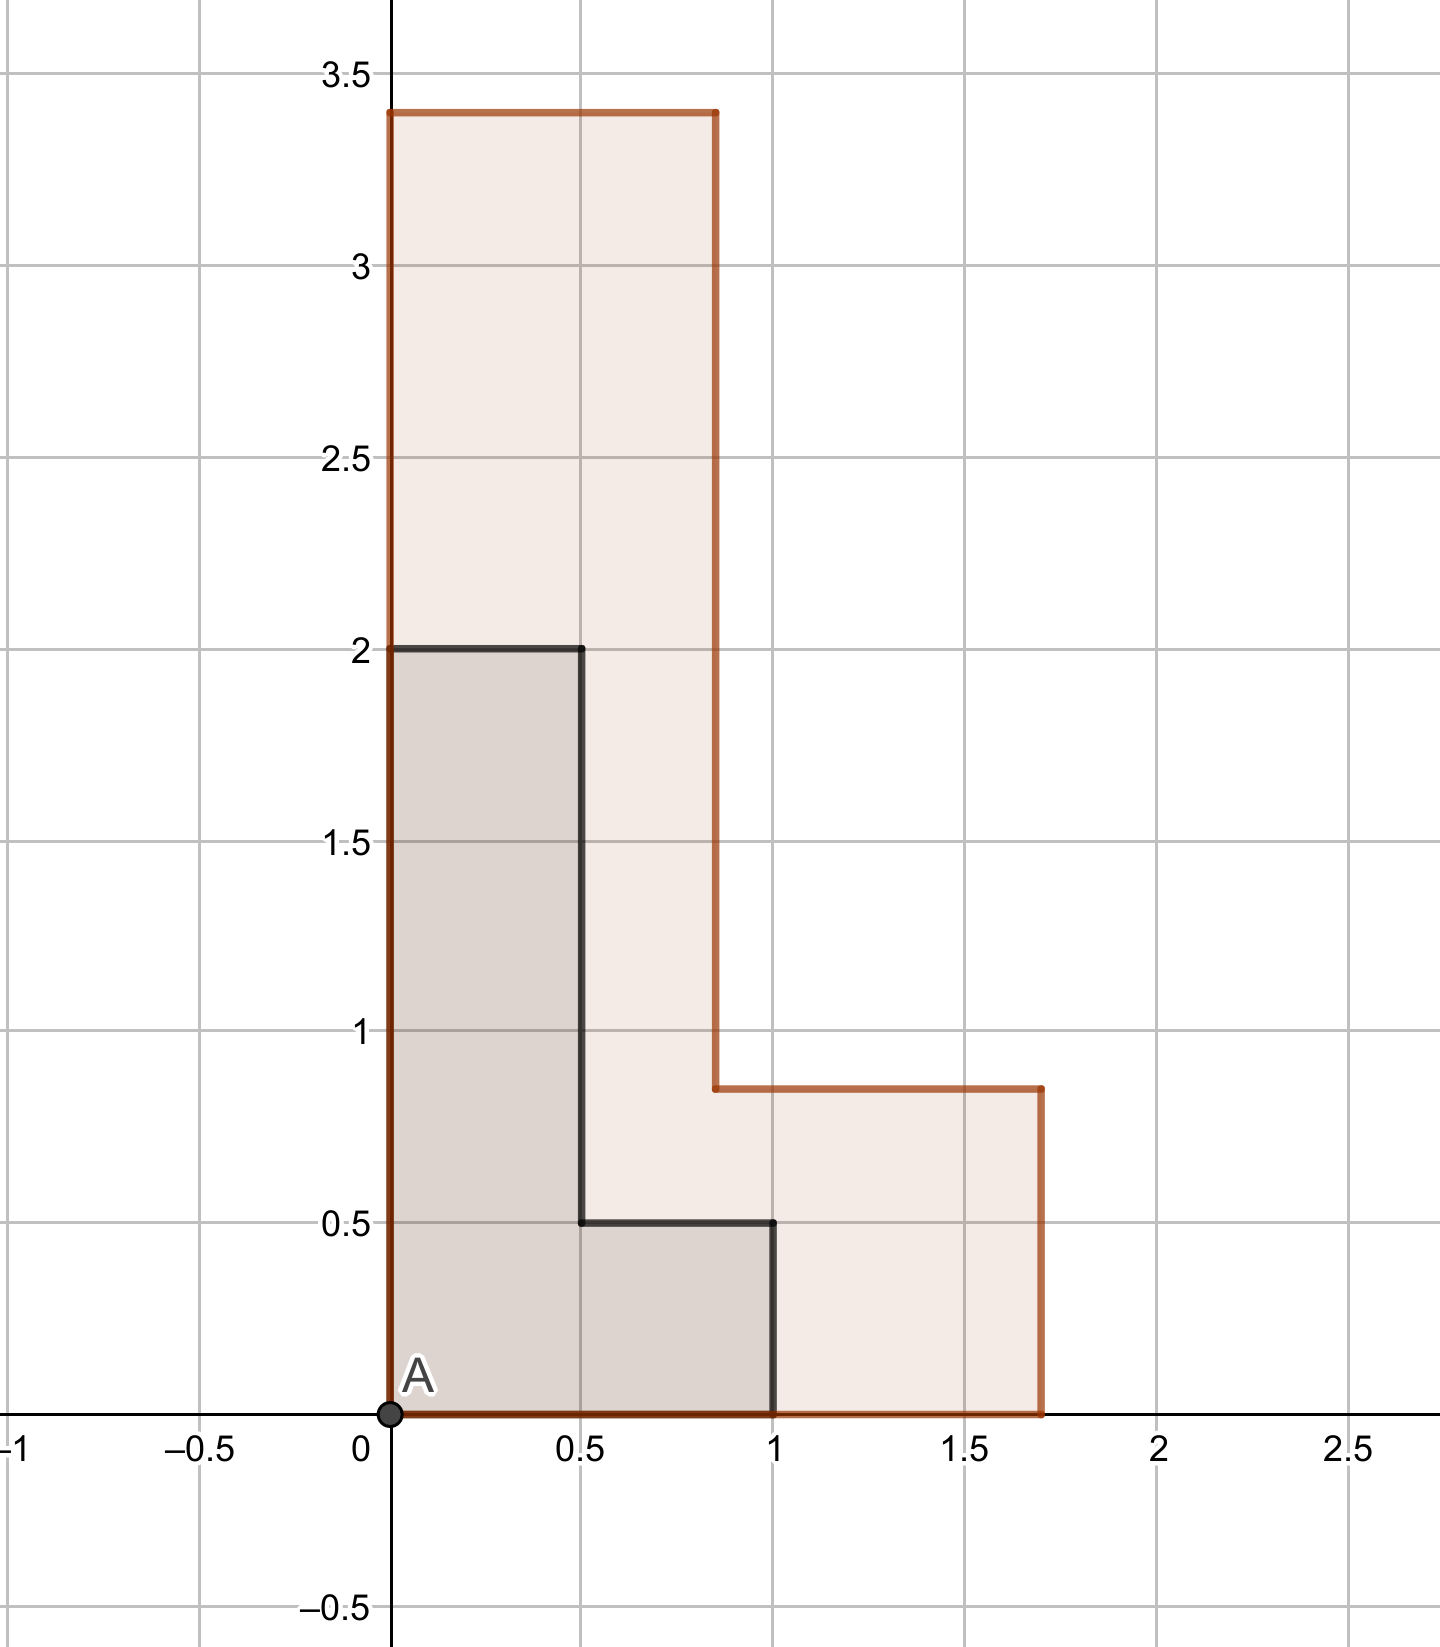
\includegraphics[height=4cm]{escalat.png}
    \caption{Una homotècia de factor 1.7.}
    \label{fig:homotecia}
\end{figure}
\subsubsection{Projeccions ortogonals}\index{projecció ortogonal}
Considerem la matriu $\begin{pmatrix}1&0\\0&0\end{pmatrix}$. Aquesta matriu envia el vector $\vec x = \begin{pmatrix}x\\y\end{pmatrix}$ a $\begin{pmatrix}x\\0\end{pmatrix}$. És a dir, projecta el vector sobre l'eix de les $x$.

Més en general, considerem una recta $\ell$ del pla, que talli l'origen. Qualsevol vector $\vec x$ es pot escriure de manera única com $\vec x = \vec x^{\parallel} + \vec x^{\perp}$, on el vector $\vec x^\parallel$ és sobre la recta $\ell$, i $\vec x^\perp$ és perpendicular a $\ell$.
\begin{definicio}
	La \index{projecció ortogonal}\emph{projecció ortogonal} respecte la recta $\ell$ és l'aplicació $\operatorname{proj}_\ell$ definida com
	\[
	\operatorname{proj}_\ell(\vec x) = \vec x^\parallel.
	\]
\end{definicio}

Observem que $\operatorname{proj}_\ell$ és una aplicació lineal (exercici).

\begin{proposicio}
	Sigui $\vec v$ un vector paral·lel a la recta $\ell$. Aleshores:
	\[
	\operatorname{proj}_\ell(\vec x) = \frac{\vec x\cdot \vec v}{\vec v\cdot \vec v} \vec v.
	\]
\end{proposicio}

També podem trobar una fórmula per la matriu de la projecció ortogonal.

\begin{proposicio}\label{prop:projR2}
	Sigui $\vec v = \begin{pmatrix}v_1\\v_2\end{pmatrix}$ un vector paral·lel a la recta $\ell$. Aleshores la matriu de $\operatorname{proj}_\ell$ és
	\[
	\frac{1}{v_1^2 + v_2^2}\begin{pmatrix}v_1^2&v_1v_2\\v_1v_2&v_2^2\end{pmatrix}
	\]
\end{proposicio}

\subsubsection{Reflexions}\index{reflexió}\label{subsubsec:reflexio}
Considerem com abans una recta $\ell$ que passi per l'origen. Volem definir la reflexió respecte la recta $\ell$. És fàcil veure que

\[
\operatorname{ref}_\ell(\vec x) = \vec x^\parallel - \vec x^\perp.
\]
Com que $\vec x = \vec x^\parallel + \vec x^\perp$, podem escriure
\[
\vec x^\parallel - \vec x^\perp = 2\vec x^\parallel - \vec x.
\]
Per tant,
\[
\operatorname{ref}_\ell = 2\operatorname{proj}_\ell - \operatorname{id}.
\]
La matriu corresponent és fàcil de trobar a partir d'aquesta fórmula:

\begin{proposicio}\label{prop:reflexio}
	Sigui $\vec v = \begin{pmatrix}v_1\\v_2\end{pmatrix}$ un vector paral·lel a la recta $\ell$. Aleshores la matriu de $\operatorname{ref}_\ell$ és
	\[
	\frac{1}{v_1^2 + v_2^2}\begin{pmatrix}v_1^2-v_2^2&2v_1v_2\\2v_1v_2&v_2^2-v_1^2\end{pmatrix}.
	\]
\end{proposicio}
Fixem-nos que la matriu de $\operatorname{ref}_\ell$ té la forma $\begin{pmatrix*}[r]a&b\\b&-a\end{pmatrix*}$, i que a més les entrades satisfan $a^2 + b^2 = 1$. De fet, es pot veure que qualsevol matriu d'aquesta forma és la matriu d'una reflexió.

\begin{figure}[h]
    \centering
    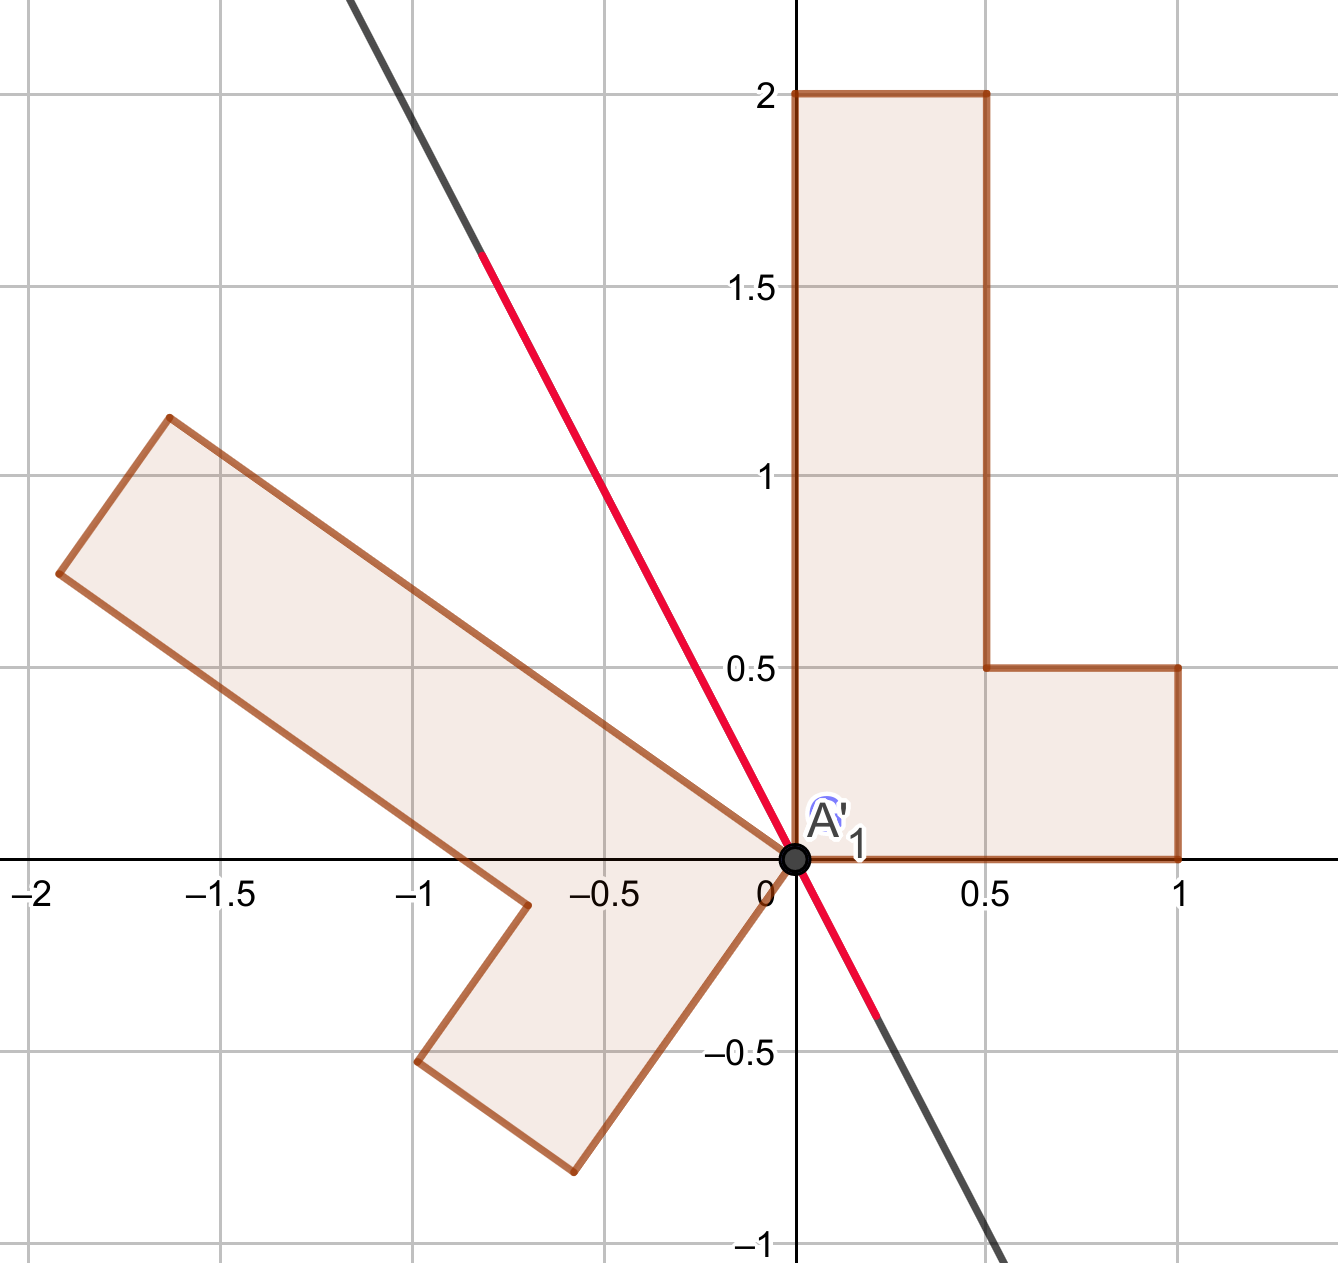
\includegraphics[height=5cm]{reflexio.png}
    \caption{Una reflexió respecte una recta. També hi podem observar la projecció a la mateixa recta.}
    \label{fig:reflexio}
\end{figure}
\subsubsection{Rotacions}\index{rotació}\label{subsubsec:rotacio}
Les matrius de la forma
\[
\begin{pmatrix*}[r]
\cos\theta&-\sin\theta\\
\sin\theta&\cos\theta
\end{pmatrix*}
\]
corresponen a una rotació d'angle $\theta$. Observem que aquesta matriu és de la forma
\[
\begin{pmatrix*}[r]
a&-b\\b&a
\end{pmatrix*},\quad a^2+b^2=1
\]
i totes les matrius d'aquesta forma són rotacions.

\begin{figure}[ht]
    \centering
    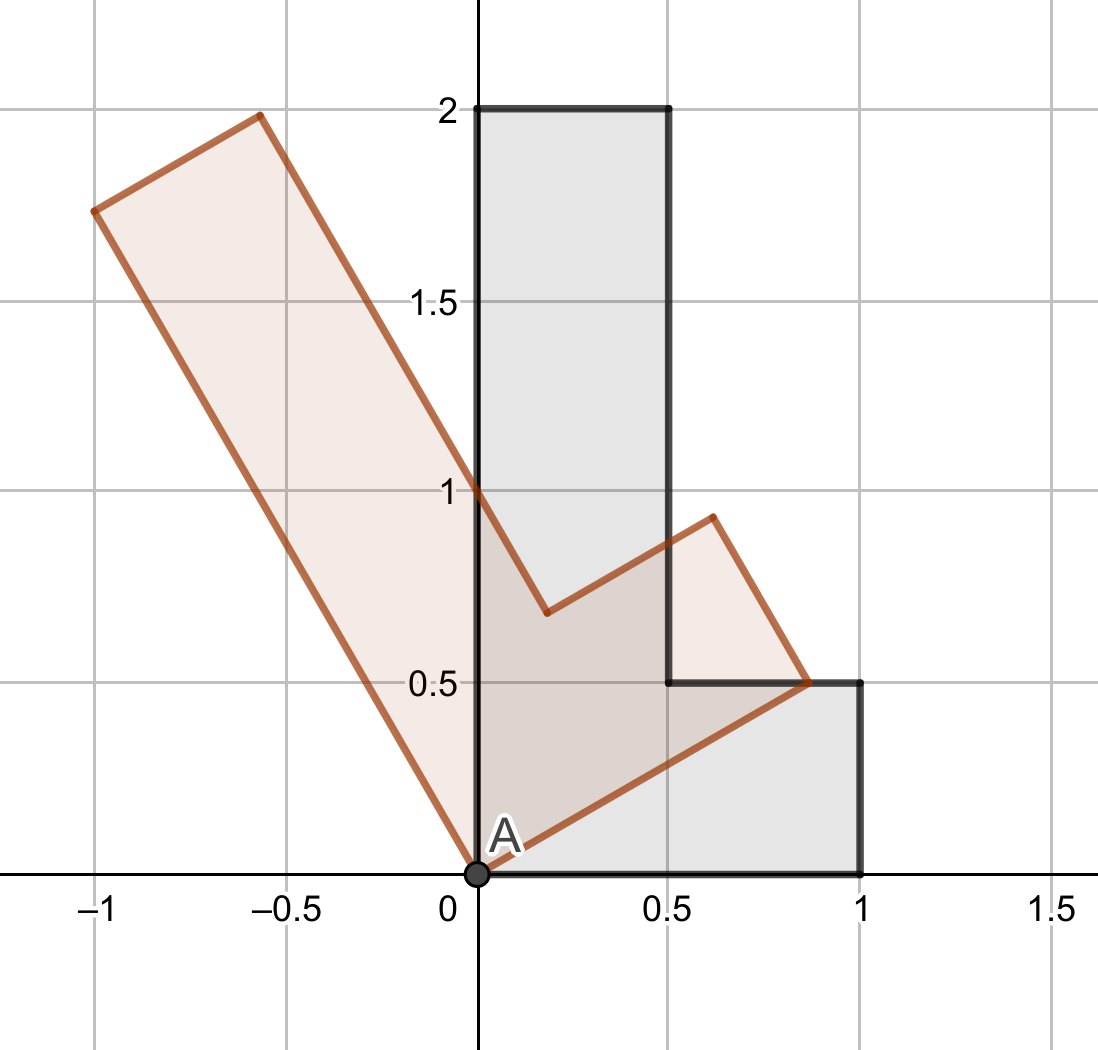
\includegraphics[height=4cm]{rotacio.png}
    \caption{Una rotació de $30^\circ$.}
    \label{fig:rotacio}
\end{figure}
\begin{exercici}
	Considereu la matriu de rotació d'angle $\theta_1$ i la de rotació d'angle $\theta_2$. Descriviu la composició d'aquestes dues aplicacions i, fent servir el producte de matrius, redescobriu les fórmules per la duplicació d'angles que heu vist a secundària.
\end{exercici}

\begin{proposicio}
	Una matriu de la forma $\begin{pmatrix*}[r]a&-b\\b&a\end{pmatrix*}$ és la composició d'una homotècia de magnitud $k=\sqrt{a^2+b^2}$ amb una rotació d'angle $\arctan(b/a)$ (si $a$ és positius) o $\arctan(b/a) + \pi$ (si $a$ és negatiu).
\end{proposicio}

\subsubsection{Lliscaments}\index{lliscament}
Per últim estudiarem les matrius de la forma $\begin{pmatrix} 1&k\\0&1\end{pmatrix}$, on $k\in \R$. Aquestes matrius fixen el vector $\vec e_1$, mentre envien el vector $\vec e_2$ a $\begin{pmatrix}k\\1\end{pmatrix}$. Geomètricament, enviarien un quadrat en el pla a un rombe, on la base es manté fixa però els costats verticals s'esbiaixen. Direm que és un lliscament horitzontal.

De manera anàloga, la matriu $\begin{pmatrix}1&0\\k&1\end{pmatrix}$ representa un lliscament vertical.

\begin{figure}[ht]
    \centering
    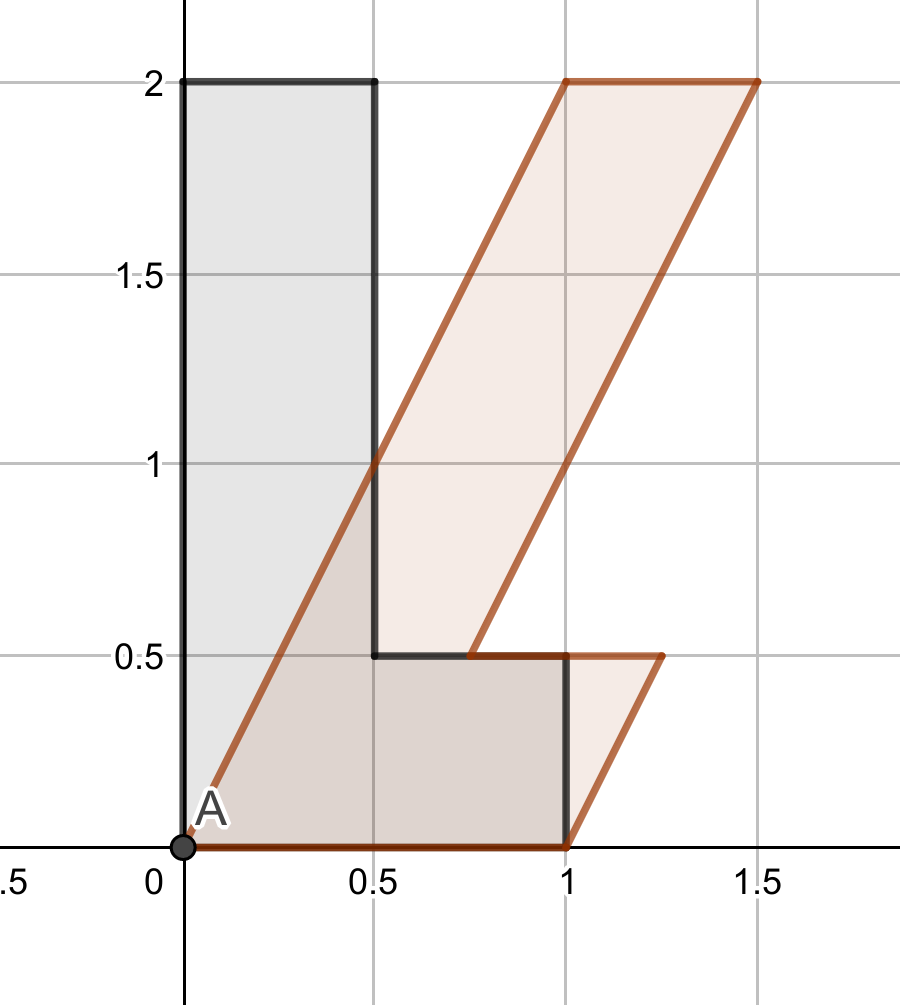
\includegraphics[height=4cm]{hshear.png}
    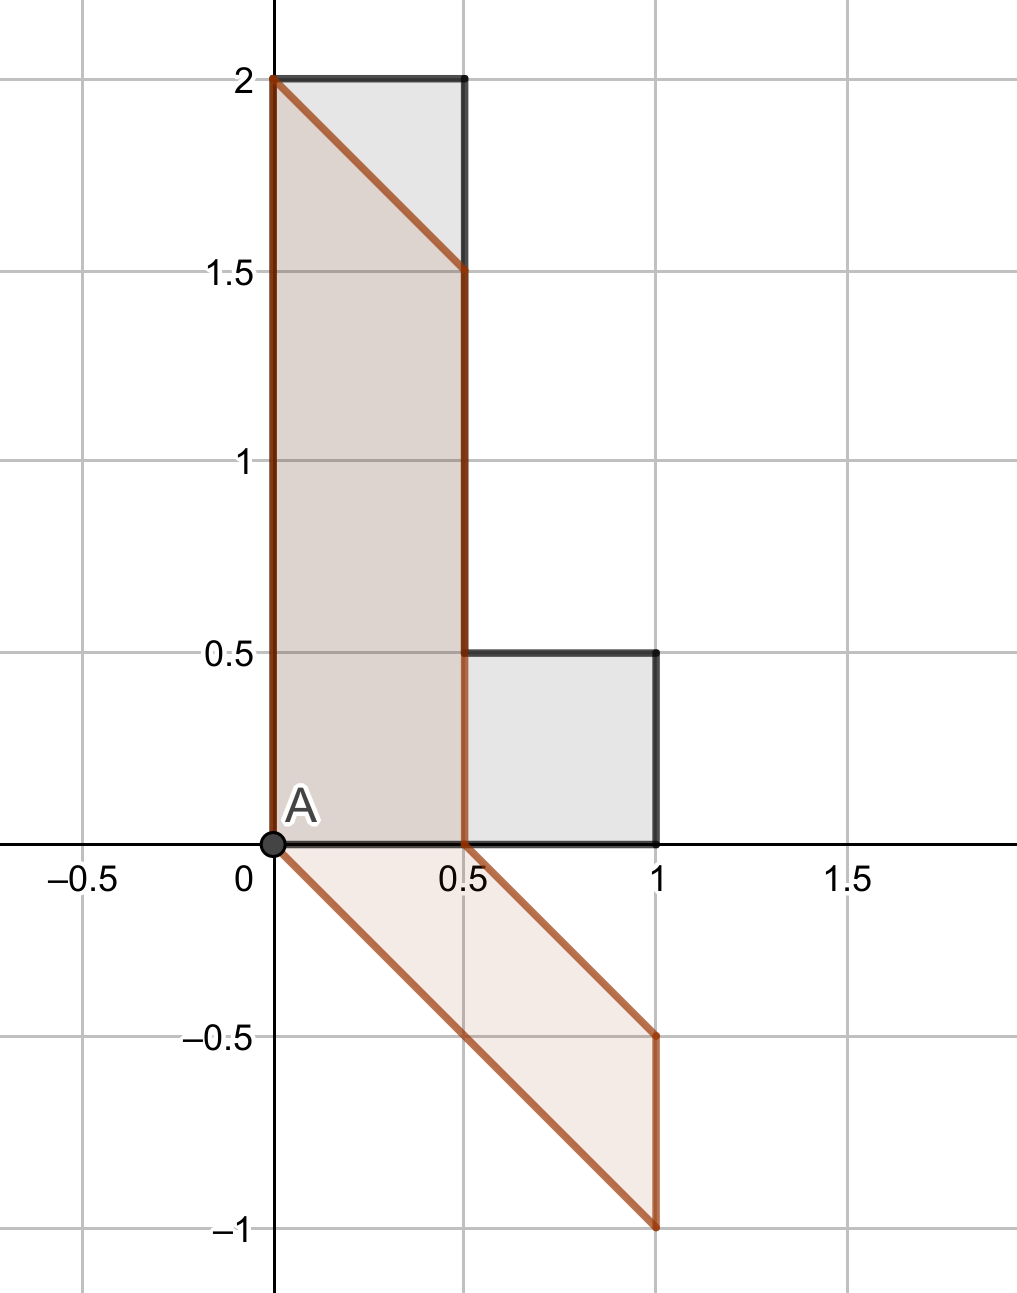
\includegraphics[height=4cm]{vshear.png}
    \caption{Lliscament horitzontal de valor $\frac 1 2$ i lliscament vertical de valor $-1$.}
    \label{fig:lliscaments}
\end{figure}

\begin{exercici}
	Calculeu, en els casos que es pugui, les inverses de les matrius corresponents a homotècies, projeccions ortogonals, reflexions i lliscaments.
\end{exercici}

\subsection{Subespais, generadors i bases}
Tornem ara a considerar $\K^n$ i les aplicacions lineals $f\colon \K^n\to\K^m$.

\begin{definicio}\label{def:subespai}
	Diem que un subconjunt \emph{$W\subset \K^n$ és un subespai vectorial}\index{subespai vectorial} si $W$ compleix que:
	\begin{itemize}
	    \item $\vec 0 \in W$,
		\item $\vec u+\vec v \in W$ per a tot $\vec u$ i $\vec v$ de $W$, i
		\item $\lambda \vec u\in W$ per a tot $\vec u\in W$ i $\lambda\in\K$.
	\end{itemize}
\end{definicio}
\begin{exemple}
	\begin{itemize}
		\item A l'$\R$-espai vectorial $\R^3$ hi considerem $F=\{(x,y,z) \in \R^3 \mid z=0\}$. Podem comprovar que és un subespai vectorial.
		\item Més en general, si tenim un sistema d'equacions lineals homogeni amb $n$ incògnites, podem identificar una solució $(x_1,\dots,x_n)$ (l'hem escrit com una fila per comoditat) amb un vector de $\K^n$ i les solucions formen un subespai vectorial de $\K^n$.
%		\item Si considerem l'espai vectorial $\R[x]$ (els polinomis en la variable $x$ sobre $\R$) i fixem un grau $n\geq 0$, llavors els polinomis de grau més petit o igual a $n$ formen un subespai.
	\end{itemize}
\end{exemple}

Com a cas particular de subespai vectorial tenim el següent:
\begin{definicio}\label{def:subespaigenerat}
	Si $\{\vec v_1, \dots \vec v_m\}\subset \K^n$, definim el \emph{subespai generat per $\{\vec v_1, \dots \vec v_m\}$} com els vectors de $\K^n$ que es poden escriure com a combinació lineal de $\{\vec v_1, \dots \vec v_m\}$. Denotem aquest subconjunt com $\langle \vec v_1, \dots \vec v_m \rangle$, i per tant tenim:
	$$
	\langle \vec v_1, \dots \vec v_m \rangle = \{\lambda_1 \vec v_1 + \cdots + \lambda_m\vec v_m \mid \lambda_i\in\K \}
	$$
\end{definicio}
\begin{observacio}
	Si $\{\vec v_1, \dots \vec v_m\}\subset \K^n$, llavors $\langle \vec v_1, \dots \vec v_m \rangle$ és un subespai vectorial.
\end{observacio}
\begin{proof} Per simplificar la notació, definim 
	$$
	W:=\langle \vec v_1, \dots \vec v_m \rangle .
	$$
	Cal veure que si $\vec u, \vec w \in W$, llavors $\vec u+\vec w \in W$: per definició d'$W$, tenim que existeixen escalar $\lambda_1, \dots ,\lambda_m$ i $\mu_1,\dots,\mu_m$ tals que $\vec u= \lambda_1 \vec v_1+\cdots +\lambda_m\vec v_m$ i $\vec w=\mu_1\vec v_1+\cdots +\mu_m\vec v_m$. Llavors, tenim que:
	$$
	\vec u+\vec w = (\lambda_1+\mu_1)\vec v_1 + \cdots + (\lambda_m+\mu_m)\vec v_m ,
	$$
	obtenint que $\vec u+\vec v \in W$.
	
	Ara considerem $\lambda \in \K$ i $\vec u\in W$. Volem veure $\lambda \vec u \in W$: com que $\vec u\in W$, existeixen $\mu_1, \dots , \mu_m\in\K$ tals que $\vec u=\lambda_1\vec v_1 + \cdots + \lambda_m\vec v_m$. Llavors:
	$$
	\lambda \vec u = (\lambda \mu_1)\vec v_1 + \cdots + (\lambda \mu_m)\vec v_m ,
	$$
	pel que $\lambda \vec u \in W$.
\end{proof}
\begin{exemple}
	Considerem $\R^3$ com a $\R$-espai vectorial i els vectors (els escrivim per files) $\{(1,0,0),(0,1,0)\}$, tenim que $\langle (1,0,0),(0,1,0)\rangle$ són els vectors d'$\R^3$ amb tercera coordenada zero.
\end{exemple}

\begin{definicio}\label{def:nucliimatge}
	Sigui $f\colon \K^n \to \K^m$ una aplicació lineal.
	\begin{itemize}
		\item Definim el \emph{nucli d'$f$}\index{nucli d'una aplicació lineal} (i el denotem com $\Ker(f)$) com el conjunt format pels vectors $\vec v\in \K^n$ tals que $f(\vec v)=\vec 0$.
		\item Definim la \emph{imatge d'$f$}\index{imatge d'una aplicació lineal} (i la denotem com $\Ima(f)$) com el conjunt dels vectors $\vec w\in\K^m$ tals que existeix $\vec v\in \K^n$ tal que $f(\vec v)=\vec w$.
	\end{itemize}
\end{definicio}
\begin{proposicio}
	Si $f \colon \K^n \to \K^m$ és una aplicació lineal, llavors:
	\begin{itemize}
		\item $\Ker(f)$ és un subespai vectorial de $\K^n$.
		\item $\Ima(f)$ és un subespai vectorial de $\K^m$.
	\end{itemize}
\end{proposicio}
\begin{proof}
	Comprovem primer que $\Ker(f)$ compleix les dues condicions de la Definició \ref{def:subespai}:
	Considerem $\vec u, \vec v \in \Ker(f)$, per tant $f(\vec u)=f(\vec v)=\vec 0$. Llavors:
	$$
	f(\vec u+\vec v)=f(\vec u)+f(\vec v)=\vec 0+\vec 0 =\vec 0 ,
	$$
	per tant $\vec u+\vec v \in \Ker(f)$.\\
	També, si $\vec u \in \Ker(f)$ i $\lambda\in\K$, llavors $f(\lambda \vec u)=\lambda f(\vec u)=\lambda \vec 0=\vec 0$, per tant $\lambda \vec u\in\Ker(f)$.
	
	Comprovem ara que $\Ima(f)$ també compleix les dues condicions: si $\vec v_1,\vec v_2 \in\Ima(f)$, llavors existeixen $\vec u_1, \vec u_2 \in \K^n$ tals que $f(\vec u_1)=\vec v_1$ i $f(\vec u_2)=\vec v_2$. Llavors es compleix que $f(\vec u_1+\vec u_2)=f(\vec u_1)+f(\vec u_2)=\vec v_1+\vec v_2$, pel que $\vec v_1+\vec v_2 \in \Ima(f)$. També, si $\vec v\in \Ima(f)$ (per tant existeix $\vec u\in \K^n$ tal que $f(\vec u)=\vec v$) i $\lambda\in\K$, tenim que $f(\lambda \vec u)=\lambda f(\vec u)=\lambda \vec v$, pel que $\lambda \vec v \in \Ima(f)$.
\end{proof}
Com a cas particular podem considerar les aplicacions $f_A\colon \K^n\to\K^m$ definides a la Subsecció \ref{subsec:matriusapl} mitjançant una matriu $A\in M_{m\times n}(\K)$. En aquest cas tenim que: 
\begin{itemize}
    \item $\Ker(f_A)$ són les solucions del sistema homogeni que té per matriu associada $A$.
    \item $\Ima(f_A)$ és el subespai de $\K^m$ generat per les columnes d'$A$ pensades com a vectors de $\K^m$.
\end{itemize}

\begin{exemple}
    Considerem $W=\{(x,y,z)\in\R^3 \mid 2x+y-z=0 \text{ i } x -y +2z=0\}$. Podem pensar que $W$ és el nucli de $f_A$, on $A=\big(\begin{smallmatrix} 2 & \phantom{-}1 & -1 \\ 1 & -1 & \phantom{-}2\end{smallmatrix}\big)$. 
\end{exemple}


Tot i que ja hi ha una definició d'independència lineal a la Definició \ref{def:dependlineal}, vegem-ne una d'equivalent:
\begin{definicio}\label{def:indeplin}
	Diem que $\{\vec v_1, \dots , \vec v_n\} \subset \K^m$, són una família de vectors \emph{linealment independents} si l'única manera d'escriure el vector zero com a combinació lineal de $\vec v_1, \dots \vec v_n$ és amb tots els coeficients zero. O sigui, si:
	$$
	\vec 0 = \lambda_1 \vec v_1+\cdots +\lambda_n\vec v_n \text{ amb $\lambda_i\in\K$} \, \Longrightarrow \, \lambda_1=\cdots =\lambda_n=0 \,.
	$$
\end{definicio}
\begin{observacio}
	Les definicions \ref{def:dependlineal} i \ref{def:indeplin} són equivalents.
\end{observacio}
\begin{proof} En realitat, veurem que negar una de les definicions és si i només si es nega l'altra:
	
	Considerem $\{\vec v_1, \dots , \vec v_n\} \subset \K^m$ que no compleixen la definició de independència lineal de la Definició \ref{def:dependlineal}, llavors un dels vectors es pot escriure com a combinació lineal dels altres. Com que els podem reordenar, considerem que $\vec v_1=\lambda_2\vec v_2+\cdots \lambda_n\vec v_n$. Llavors
	$$
	\vec 0 = \vec v_1- \lambda_2 \vec v_2 - \cdots -\lambda_n\vec v_n 
	$$
	i el vector zero es pot escriure com a combinació lineal de $\{\vec v_1, \dots , \vec v_n\}$ amb, com a mínim, un coeficient no nul (el de $\vec v_1$).
	
	Considerem $\{\vec v_1, \dots , \vec v_n\} \subset \K^n$ que no compleixen la definició de independència lineal de la Definició \ref{def:indeplin}, llavors podem escriure el vector zero:
	$$
	\vec 0 = \lambda_1\vec v_1+ \lambda_2 \vec v_2 + \cdots +\lambda_n\vec v_n 
	$$
	amb algun $\lambda_i\neq 0$. Com que els podem reordenar, considerem que $\lambda_1\neq 0$. Llavors:
	$$
	\vec v_1 = -(\lambda_2/\lambda_1) \vec v_2 - \cdots -(\lambda_n/\lambda_1)\vec v_n 
	$$
	i el vector $\vec v_1$ és combinació lineal de la resta.
\end{proof}
\begin{observacio}\label{obs:linindep}
	Si $\{\vec v_1, \dots \vec v_n\}\subset \K^m$, és una família de vectors linealment independents, llavors qualsevol subfamília d'aquesta també ho serà. Per tant, treure vectors preserva la propietat de ser linealment independents.
\end{observacio}

Podem veure si una família de vectors és linealment independent mirant el nucli d'una aplicació lineal:
\begin{proposicio}
    Siguin $\{\vec v_1, \dots, \vec v_n\}\subset \K^m$ una família de vectors i $A\in M_{m\times n}(\K)$ la matriu que té per columnes els vectors $\vec v_j$. Llavors $\{\vec v_1, \dots, \vec v_n\}$ són linealment independents si, i només si, $\Ker(f_A)=\{\vec 0\}$.
\end{proposicio}
\begin{proof}
    Observem que donar una combinació lineal $x_1\vec v_1+ \cdots+x_n \vec v_n$ és equivalent a multiplicar $AX$, on $X$ és el vector columna que té per coeficients $x_1, \dots, x_n$. 
    
    llavors, que $\{\vec v_1, \dots, \vec v_n\}$ siguin linealment independents vol dir que la única manera d'obtenir $AX=\vec 0$ és amb $X=\vec 0$, o, el que és el mateix, $\Ker(f_A)=\vec 0$. 
\end{proof}

Podem veure quants vectors linealment independents hi ha dins d'una família de vectors mirant el rang de la matriu corresponent:
\begin{lema}\label{lema:rangiLI}
    Si $\vec v_1, \dots ,\vec v_n\in\K^m$ són vectors, llavors el nombre màxim de vectors linealment independents continguts a $\{\vec v_1, \dots ,\vec v_n\}$ és el rang de la matriu $A$ que té per columnes els vectors $\vec v_i$. 
\end{lema}
\begin{proof}
    Anomenem $k$ al nombre màxim de vectors linealment independents a $\{\vec v_1, \dots ,\vec v_n\}$. Com que l'ordre no és important, reordenem els vectors $\{\vec v_1, \dots ,\vec v_n\}$ tal que els $k$ primers són linealment independents i que qualsevol altre $\vec v_j$ amb $j\geq k$, $\{\vec v_1, \dots ,\vec v_k,\vec v_j\}$ no són linealment independents. Sigui $B$ la matriu que té per columnes els vectors $\vec v_1, \dots, \vec v_k$ i $\overline{B_j}$ la que té per columnes els vectors $\vec v_1, \dots, \vec v_k,\vec v_j$. Pensem $\overline{B_j}$ com la matriu ampliada d'un sistema d'equacions, amb $B$  matriu associada. Com que $\vec v_j$ és combinació lineals dels $\vec v_1, \dots, \vec v_k$, el sistema té solució i $\Rang(B)=\Rang(\overline{B_j})$.\\
    Podem iterar aquest procediment amb els altres vectors $\vec v_{j}$ amb $j\geq k$ i obtenim que $\Rang(B)=\Rang(A)$.\\
    Finalment, com que $B$ té per columnes vectors linealment independents, el sistema d'equacions homogeni que té per matriu associada $B$, té solució única, i per tant $\Rang(B)=k$ (el número d'incògnites).
\end{proof}
D'aquí podem deduir una propietat que relaciona el producte de matrius amb el rang:
\begin{corollari}
Si $A\in M_{m\times n}(\K)$ i $B\in M_{n\times r}(\K)$, llavors:
$$
\Rang(AB)\leq \min\{\Rang(A),\Rang(B)\}
$$
\end{corollari}
\begin{proof} 
%    $A$ indueix una aplicació lineal $f_A\colon \K^n\to \K^m$, $B$ indueix una altra aplicació lineal $f_B\colon \K^r\to \K^n$ i hem vist que $AB$ indueix una aplicació lineal que es correspon amb la composició $f_B\circ f_A$.\\
    Les columnes d'$AB$ es poden pensar com a combinació lineal de columnes d'$A$, per tant no n'hi pot haver més de linealment independents, obtenint $\Rang(AB)\leq\Rang(A)$.\\
    Si ara transposem les matrius i fem el mateix raonament, tenim que $$\Rang(AB)=\Rang((AB)^T)=\Rang(B^TA^T)\leq \Rang(B^T)=\Rang(B)$$
    Per tant $\Rang(AB)$ és més petit que el rang d'$A$ i que el rang de $B$.
\end{proof}

 \begin{corollari}\label{cor:maximLI}
     Si $\{\vec v_1, \dots, \vec v_n\}\subset \K^m$ són linealment independents, llavors $n\leq m$. 
 \end{corollari}
 \begin{proof}
    Si $\{\vec v_1, \dots, \vec v_n\}$ són linealment independents, pel Lema \ref{lema:rangiLI}, la matriu $V$, una matriu que té per columnes els vectors $\vec v_j$ té rang $n$. Això només es pot tenir si hi ha com a mínim $n$ files, i per tant $m\geq n$.
\end{proof}


Vegem ara el concepte de \emph{generadors}:
\begin{definicio}\label{def:sistgen}
	Si $\{\vec v_1, \dots \vec v_n\}\subset \K^m$ són tals que $\K^m=\langle \vec v_1, \dots \vec v_n\rangle$, diem que \emph{$\{\vec v_1, \dots \vec v_n\}$ són un sistema de generadors de $\K^m$}\index{sistema de generadors}.
	
	Si $W\subset \K^n$ és un subespai vectorial i $\{\vec v_1, \dots \vec v_n\}\subset W$ són tals que $W=\langle \vec v_1, \dots \vec v_n\rangle$, diem que \emph{$\{\vec v_1, \dots \vec v_n\}$ són un sistema de generadors de $W$}.
\end{definicio}
\begin{observacio}\label{obs:sisgen}
	Si $\{\vec v_1, \dots \vec v_n\}\subset \K^m$ és un sistema de generadors i hi afegim un vector $\vec u$, llavors $\{\vec u,\vec v_1, \dots \vec v_n\}\subset \K^m$ és també un sistema de generadors. O sigui, afegir vectors conserva la propietat de ser \emph{sistema de generadors}.
\end{observacio}
\begin{observacio}
	Si $\{\vec v_1, \dots \vec v_n\}\subset \K^m$, llavors $\{\vec v_1, \dots \vec v_n\}$ són un sistema de generadors de $\langle \vec v_1, \dots \vec v_n\rangle$ (que és un subespai vectorial).
\end{observacio}
Vegem algunes propietats dels sistemes de generadors:
\begin{lema}\label{lem:generadors}
	Si $\vec v_1, \dots , \vec v_n, \vec u$ són vectors de $\K^m$, llavors:
	\begin{enumerate}[\rm (a)]
		\item $\vec u\in \langle \vec v_1, \dots , \vec v_n \rangle$ si i només si $\langle \vec v_1, \dots , \vec v_n \rangle=\langle\vec u, \vec v_1, \dots , \vec v_n \rangle$.
		\item Si $\vec u = \lambda_1 \vec v_1 + \cdots + \lambda_n \vec v_n$ i $i$ és un índex tal que $\lambda_i\neq 0$, llavors:
		$$\langle \vec v_1,\dots,\vec v_{i-1},\vec v_i , \vec v_{i+1}, \dots , \vec v_n\rangle=\langle \vec v_1, \dots,\vec v_{i-1},\vec u , \vec v_{i+1},\dots,\vec v_n\rangle.$$ 
	\end{enumerate}
\end{lema}
\begin{proof}
	Comencem demostrant (a):\\
	Suposem $\vec u\in \langle \vec v_1, \dots , \vec v_n \rangle$, per tant existeixen $\lambda_1, \dots, \lambda_n\in\K$ tals que $\vec u=\lambda_1\vec v_1+\dots \lambda_n\vec v_n$. 
	Sempre tenim $\langle \vec v_1, \dots , \vec v_n \rangle\subset\langle\vec u, \vec v_1, \dots , \vec v_n \rangle$, per tant cal comprovar l'altre inclusió. Sigui $\vec w \in \langle\vec u, \vec v_1, \dots , \vec v_n \rangle$, per tant existeixen $\mu,\mu_1,\dots \mu_n\in\K$ tals que $\vec w=\mu \vec u+\mu_1\vec v_1+\dots \mu_n\vec v_n$. Utilitzant que $\vec u=\lambda_1\vec v_1+\dots \lambda_n\vec v_n$, tenim:
	$$
	\vec w=(\mu\lambda_1+\mu_1)\vec v_1+\dots (\mu\lambda_n+\mu_n)\vec v_n ,
	$$
	per tant $w \in \langle \vec v_1, \dots , \vec v_n \rangle$.
	
	En canvi, si $\vec u\notin \langle \vec v_1, \dots , \vec v_n \rangle$, com que sempre tenim $\vec u\in \langle\vec u, \vec v_1, \dots , \vec v_n \rangle$, obtenim que $\langle \vec v_1, \dots , \vec v_n \rangle\neq\langle\vec u, \vec v_1, \dots , \vec v_n \rangle$.
	
	Per demostrar (b) comencem observant que, com que $\lambda_i\neq 0$, 
	$$v_i=(1/\lambda_i) \vec u -(\lambda_1/\lambda_i) \vec v_1- \cdots-(\lambda_{i-1}/\lambda_i) \vec v_{i-1} - (\lambda_{i+1}/\lambda_i) \vec v_{i+1} - \cdots -(\lambda_n/\lambda_i) \vec v_n
	$$
	pel que $\vec v_1 \in \langle \vec v_1, \dots,\vec v_{i-1},\vec u , \vec v_{i+1},\dots,\vec v_m\rangle$. Apliquem ara dos cops (a) per obtenir (l'ordre en que s'escriuen els vectors en un sistema de generadors no importa):
	$$
	\langle \vec v_1, \dots , \vec v_n\rangle=
	\langle \vec u,\vec v_1, \dots, \vec v_i, \dots , \vec v_n\rangle=
	\langle \vec v_1, \dots,\vec v_{i-1},\vec u , \vec v_{i+1},\dots,\vec v_n\rangle.
	$$
\end{proof}
Vegem ara quin és el nombre mínim de vectors generadors de $\K^m$:
\begin{lema}\label{lema:genKn}
    Si $\{\vec v_1, \dots, \vec v_n\}\subset \K^m$ són un sistema de generadors, llavors $n\geq m$.
\end{lema}
\begin{proof}
    Considerem els vectors estàndard $\vec e_j\in\K^m$ definits a la Subsecció \ref{subsec:matriusapl}. Com que $\langle \vec v_1, \dots, \vec v_n \rangle=\K^m$, tenim que $\vec e_j \in \langle \vec v_1, \dots, \vec v_n \rangle$, per tant, existeixen $x_{1j}, \dots, x_{nj}$ tals que $x_{1j} \vec v_1+ \cdots+x_{nj}\vec v_n=\vec e_j$. Podem escriure aquesta igualtat de forma matricial:
    $$
    A X = \1_m
    $$
    on $A \in M_{m\times n}(\K)$ és la matriu que té per columnes els vectors $\vec v_j$, $X\in M_{n\times m}(\K)$ és la matriu que té per coeficients $x_{ij}$ i $\1_m$ és la matriu que té per columnes els vectors $\vec e_j$ (que és la identitat).
    
    Ara utilitzem el rang: $m=\Rang(AX)\leq\Rang(A)$, per tant $A$ té com a mínim $m$ columnes i $n\geq m$.
\end{proof}

\begin{definicio}\label{def:base}
	Diem que una família ordenada de vectors $\calb=[\vec  v_1, \dots, \vec v_n]$ amb $\vec v_j\in \K^m$, és \emph{una base de $\K^m$}\index{base d'un espai vectorial} si $\{\vec v_1,\dots,\vec v_n\}$, són linealment independents i generadors de $\K^m$.
\end{definicio}
\begin{observacio}
	L'ordre dels vectors d'una base és important: de la definició es dedueix que si $[\vec  v_1, \vec v_2, \vec v_3,\dots, \vec v_n]$ és una base de $\K^m$, llavors $[\vec  v_2, \vec v_1, \vec v_3,\dots, \vec v_n]$ també ho és, però considerarem que són bases diferents.
\end{observacio}
%A l'Observació \ref{obs:sisgen} veiem que si afegim vectors a un sistema de generadors, continua sent sistema de generadors. En canvi, si en traiem, es pot perdre aquesta propietat. Respectivament, a l'Observació  \ref{obs:linindep}, hem vist que si traiem vectors a una família de vectors linealment independents, el resultat encara és linealment independent. En canvi, si n'afegim, aquesta propietat també es pot perdre.

%Considerem $\vec v_1,\dots, \vec v_m$ una família de generadors d'un $\K$-espai vectorial $E$. Suposem que no són linealment independents. Llavors un es pot escriure com a combinació lineal de la resta. Com que els podem reordenar, considerem que $\vec v_m$ es pot escriure com a combinació lineal de $\vec v_1, \dots \vec v_{m-1}$. Dit d'una altra manera $\vec v_m \in \langle \vec v_1,\dots,\vec v_{m-1}\rangle$. Aplicant el Lema \ref{lem:generadors}, tenim que:
%$$
%E=\langle \vec v_1,\dots,\vec v_m\rangle=\langle \vec v_1,\dots,\vec v_{m-1}\rangle .
%$$
%Podem iterar aquest procediment mentre tinguem vectors linealment dependents, fins que els vector que quedin siguin linealment independents. Llavors tindrem una base d'$E$.
\begin{teorema}
	Sigui $\calb=[\vec v_1, \dots, \vec v_n]$ una base de $\K^m$, llavors $m=n$. Diem que \emph{$\K^m$ té dimensió $m$}\index{dimensió}.
\end{teorema}
\begin{proof}
    Com que han de ser linealment independents, del Corol·lari \ref{cor:maximLI}, obtenim que $n\leq m$. Com que han de ser generadors, del Lema \ref{lema:genKn}, obtenim que $n\geq m$, per tant, $m=n$.
\end{proof}

\begin{exemple}
	\begin{itemize}
		\item Els vectors (ho escrivim per files) $(1,0)$ i $(0,1)$ formen una base de $\R^2$.
		\item Els vectors $(1,0)$ i $(1,1)$ també formen una base de $\R^2$.
		\item Els vectors $(1,0)$, $(0,1)$ i $(1,1)$ no formen una base de $\R^2$ (no són linealment independents).
	\end{itemize}
\end{exemple}

\begin{proposicio}
	\begin{enumerate}[\rm (a)]
		\item Si $\langle \vec v_1, \dots , \vec v_n \rangle = \K^m$, qualsevol subfamília maximal de vectors linealment independents de $\vec v_1, \dots, \vec v_n$ formaran una base de $\K^m$.
		\item Si $\vec v_1, \dots, \vec v_n \in \K^m$ és una família de vectors linealment independents, podem ampliar la família fins a obtenir una base de $\K^n$.
	\end{enumerate}
\end{proposicio}
\begin{proof}
	Demostrem primer (a): en aquest cas, maximal vol dir que si afegim qualsevol vector, la família obtinguda deixa de ser linealment independent. Suposem que tenim una família maximal de vectors linealment independents $\vec v_{i_1}, \dots ,\vec v_{i_k}$. Per demostrar que són base cal veure que són generadors i ho farem per contraposició lògica. Si no fossin generadors, tindríem:
	$$
	\langle \vec v_{i_1}, \dots ,\vec v_{i_k}\rangle \subsetneqq \langle \vec v_{1}, \dots ,\vec v_{n}\rangle
	$$
	i per tant hi hauria un $\vec v_j$ tal que $\vec v_j \not\in \langle \vec v_{i_1}, \dots ,\vec v_{i_k}\rangle$. Llavors $\vec v_{i_1}, \dots ,\vec v_{i_k}, \vec v_j$ serien linealment independents (si $\lambda_1\vec v_{i_1}+\cdots + \lambda_k\vec v_{i_k}+\lambda \vec v_j=\vec 0$, pot passar que $\lambda=0$ o $\lambda\neq0$; si $\lambda=0$, com que $\vec v_{i_1}, \dots ,\vec v_{i_k}$ són linealment independents, tots els $\lambda_i=0$; si $\lambda\neq 0$, podríem aïllar $\vec v_j$ en funció dels altres, contradient que $\vec v_j \not\in \langle \vec v_{i_1}, \dots ,\vec v_{i_k}\rangle$). Per tant, tindríem que $\vec v_{i_1}, \dots ,\vec v_{i_k}$ no seria maximal, tenint una contradicció.
	
	Per demostrar (b), considerem la família $\vec v_1,\dots,\vec v_n,\vec e_1, \dots, \vec e_m$ (on $\vec e_i$ són els vectors estàndard) i en triem una subfamília maximal que contingui els primers $k$ vectors.
\end{proof}

El resultat de l'apartat (a) també es pot llegir com que si tenim un sistema de generadors de $\K^n$, podem anar eliminant vectors fins a quedar-nos amb una base.

\begin{proposicio}\label{prop:base=li=gen}
	Si $\vec v_1, \dots, \vec v_n$ és una família de vectors de $\K^n$, llavors són equivalents:
	\begin{enumerate}[\rm (a)]
		\item $\vec v_1, \dots, \vec v_n$ formen una base.
		\item $\vec v_1, \dots, \vec v_n$ són un sistema de generadors.
		\item $\vec v_1, \dots, \vec v_n$ són linealment independents.
	\end{enumerate}
\end{proposicio}
\begin{proof}
	Tenim que per definició de base (a)$\Rightarrow$(b) i (a)$\Rightarrow$(c).
	
	Suposem que tenim (b). Si no fossin linealment independents, hi hauria una subfamília de vectors linealment independents $\vec v_{i_1}, \dots, \vec v_{i_k}$ maximals amb $k<n$, per tant tindríem una base amb $k$ elements en un espai de dimensió $n>k$, per tant contradicció. Per tant els vectors són linealment independents (i generadors), per tant tenim (a).
	
	Suposem que tenim (c). Si $\vec v_1, \dots, \vec v_n$ no fossin generadors, podríem afegir vectors fins tenir una base, però aquesta nova base tindria més de $n$ vectors, pel que contradiu que l'espai $\K^n$ sigui de dimensió $n$. Per tant $\vec v_1, \dots, \vec v_n$ són generadors (i linealment independents), per tant tenim (a).
\end{proof}
Encara podem donar una altra caracterització del concepte de base.
\begin{teorema}\label{teo:base_coord_uniq}
    Una família de vectors $\{\vec v_1, \dots, \vec v_n\} \subset \K^m$ formen una base si i només si tot per a tot vector $\vec v\in \K^m$ existeixen uns únics $\lambda_1, \dots, \lambda_n\in\K$ tals que $\vec v=\lambda_1\vec v_1+\cdots + \lambda_n\vec v_n$.
\end{teorema}
\begin{proof}
Suposem $\{\vec v_1, \dots, \vec v_n\} \subset \K^m$, llavors són generadors de $\K^m$ si i només si per a tot vector $\vec v\in \K^m$ existeixen $\lambda_1, \dots, \lambda_n\in\K$ tals que $\vec v=\lambda_1\vec v_1+\cdots + \lambda_n\vec v_n$, per tant si i només si el sistema té solució.

Suposem $\{\vec v_1, \dots, \vec v_n\} \subset \K^m$, llavors són linealment independents si i només si existeixen $\lambda_1, \dots, \lambda_n,\mu_1,\dots, \mu_n\in\K$ tals que $\lambda_1\vec v_1+\cdots + \lambda_n\vec v_n=\mu_1\vec v_1+\cdots + \mu_n\vec v_n$ implica que $\lambda_j=\mu_j$ per a tot $j$, per tant, si i només si la solució és única.
\end{proof}

\begin{observacio}
    Equivalentment al Teorema \ref{teo:base_coord_uniq}, podem dir que $\{\vec v_1, \dots, \vec v_n\} \subset \K^m$ formen una base si i només si la matriu $A\in M_{m\times n}(\K)$ formada pels vectors $\vec v_i$ a les columnes és invertible (en particular, ha de ser quadrada i per tant $n=m$).
\end{observacio}
\begin{proof}
    Si són base, necessitem que el sistema $Ax=B$ tingui solució única per a tot $B\in M_{n\times 1}$. Anem considerant $B_j=\vec e_j$ (els vectors estàndard definits a la Secció \ref{subsec:matriusapl}) i resolent cada un dels sistemes amb solucions $X_j\in M_{n\times 1}$, tindrem una matriu $X$ que compleix $AX=\1_n$, per ant $A$ és invertible.\\
    Si la matriu $A$ és invertible, $x=A^{-1}B$, per tant el sistema és compatible determinat per a tot $B$.
\end{proof}

Volem aprofitar les matrius per estudiar espais vectorials que no siguin del tipus $\K^n$. Com a cas particular, tenim els subespais. Comencem veient que el concepte de base també es pot estendre a subespais de $\K^m$. 
\begin{definicio}
Considerem $V\subset \K^m$ un subespai vectorial (Definició \ref{def:subespai}). Un conjunt ordenat de vectors $[\vec v_1, \dots, \vec v_n]$ amb $\vec v_i \in V$ són \emph{una base de $V$} si són linealment independents i generen $V$.
\end{definicio}
Podem fer les observacions següents:
\begin{proposicio}
Si $[\vec v_1, \dots, \vec v_n]$ és una base d'un subespai $V\subset \K^m$, llavors:
    \begin{enumerate}[\rm (a)]
        \item  $n\leq m$ i
        \item $n=m$ si i només si $V=\K^m$.
    \end{enumerate}
\end{proposicio}
\begin{proof}
    (a) és conseqüència del Corol·lari \ref{cor:maximLI}: si $\{ \vec v_1, \dots, \vec v_n \}$ són linealment independents a $\K^m$, llavors $n\leq m$.
    
    (b) Suposem que $n=m$, per la Proposició \ref{prop:base=li=gen}, si śon linealment independents són base de tot $\K^m$, per tant $V=\K^m$. I, si $V=\K^m$, llavors qualsevol base ha de tenir $m$ vectors, i $n=m$.
\end{proof}
\begin{observacio}
    Sigui $V$ un subespai vectorial de $\K^m$, $\{\vec u_1,\dots,\vec u_k\}\subset V$ una família de vectors linealment independents i $\{\vec v_1,\dots,\vec v_n\}\subset V$ una família de vectors generadors de $V$. Llavors $k\leq n$.
\end{observacio} 
\begin{proof}
%    Considerem $V=\langle \vec v_1,\dots,\vec v_n \rangle$ i triem una subfamília maximal de vectors linealment independents. Suposem que aquesta família té $m'$ vectors amb $n'\leq n$, i suposem són els $m'$ primers (si cal els reordenem). Per tant tenim $\{\vec v_1,\dots,\vec v_{n'}\}$ generadors de $V$ i linealment independents.
    
%    Suposem $k>n$, i per tant $k>n'$, i volem arribar a contradicció:
    Com que $\vec u_1\in V=\langle \vec v_1,\dots,\vec v_n \rangle$, existeixen $\lambda_i\in\K$ tals que $\vec u_1=\lambda_1 \vec v_1+\cdots+\lambda_n\vec v_n$. Com que $\vec u_1 \neq\vec 0$ (el $\vec 0$ no forma part de cap família de vectors linealment independents), existeix $\lambda_i\neq 0$. Si cal, reordenem els vectors $\vec v_1,\dots,\vec v_n$ i suposem $\lambda_1\neq 0$. Aplicant ara el Lema \ref{lem:generadors}, tenim:
    $$
    V=\langle \vec v_1,\dots,\vec v_n \rangle=\langle \vec u_1,\vec v_2,\dots,\vec v_n \rangle .
    $$
    Considerem ara $\vec u_2$: com que  $\vec u_2\in V=\langle \vec u_1,\vec v_2,\dots,\vec v_n \rangle$, existeixen $\mu_1\in\K$ i $\lambda_i\in\K$ $(i\geq 2)$ tals que $\vec u_1=\mu_1\vec u_1+\lambda_2\vec v_2+\cdots+\lambda_n\vec v_n$. Com que $\{\vec u_1,\vec u_2\}$ són linealment independents, existeix $\lambda_i$ tal que $\lambda_i\neq 0$ amb $i\geq 2$. Si cal, podem reordenar els vectors $\{\vec v_2,\dots,\vec v_n\}$ i suposar que $\lambda_2\neq 0$. Tornem a aplicar el Lema \ref{lem:generadors} i obtenim:
    $$
    V=\langle \vec u_1,\vec v_2,\dots,\vec v_{n} \rangle=\langle \vec u_1,\vec u_2,\vec v_3,\dots,\vec v_{n} \rangle .
    $$
    Iterem ara aquest procediment. Si $k>n$, llavors podem iterar el procediment amb els $n$ primers vectors de $\{\vec u_1,\dots,\vec u_k\}$, obtenint:
    $$
    V=\langle \vec u_1,\vec u_2,\dots,\vec u_{n} \rangle
    $$
    i per tant $\vec u_{n+1} \in V=\langle \vec u_1,\vec u_2,\dots,\vec u_{n} \rangle$, que contradiu el fet de que $\{\vec u_1, \dots, \vec u_n,\vec u_{n+1}\}$ siguin linealment independents.
\end{proof}
\begin{teorema}
\label{teo:bases-igual-cardinalitat}
    Si $V\subset \K^m$ és un subespai vectorial, totes les bases de $V$ tenen el mateix nombre d'elements i l'anomenem \emph{dimensió de $V$}\index{dimensió}.
\end{teorema}
\begin{proof}
Suposem que tenim $\calb_1=[\vec u_1,\dots,\vec u_k]$ i $\calb_2=[\vec v_1,\dots,\vec v_n]$ dues bases de $V$. Com que els vectors de $\calb_1$ són linealment independents i els de $\calb_2$ generadors de $V$, $k\leq n$. Com que els vectors de $\calb_1$ són generadors de $V$ i $\calb_2$ són linealment independents, $k\geq n$. Per tant $k=n$.
\end{proof}
Veiem que aquests resultats són molt semblants als que obteníem per $\K^n$ i els podem resumir a:
\begin{teorema}\label{teo:baseV}
    Si $V$ és un subespai de $\K^m$ de dimensió $n$, llavors:
    \begin{enumerate}[\rm (a)]
        \item $n$ és el nombre màxim que pot tenir una família de vectors linealment independents de $V$.
        \item $n$ és el nombre mínim que pot tenir una família de vectors generadors de $V$.
        \item $n$ vectors de $V$ són linealment independents si i només si són generadors de $V$, si i només si són base de $V$.
    \end{enumerate}
\end{teorema}
\begin{proof}
Només cal veure (c), i de (c) que $\vec v_1, \dots , \vec v_n$ són linealment independents si i només si generen $V$: si són linealment independents, i no generen $V$, podem trobar un vector $\vec u\not\in\langle \vec v_1,\dots, \vec v_n\rangle$, per tant $\{\vec u, \vec v_1,\dots,\vec v_n\}$ és una família de vectors linealment independents que té $n+1$ vectors, contradient (a). Si $\vec v_1, \dots , \vec v_n$ són generadors i no són linealment independents, vol dir que un d'ells es pot escriure com ca combinació lineal dels altres, i per tant tindríem una família de vectors generadors amb $n-1$ vectors, que no pot ser.
\end{proof}

Aprofitem tots aquests continguts per a veure com es pot trobar una base de la imatge d'$f\colon \K^n\to \K^m$, una aplicació lineal:
\begin{lema}\label{lema:imfA}
    Si $f\colon \K^n \to K^m$ és una aplicació lineal i $A$ la matriu tal que $f=f_A$, llavors $\Ima(f)=\langle f(\vec e_1), \dots, f(\vec e_n) \rangle$ i $\dim(\Ima(f))=\Rang(A)$.
\end{lema}
\begin{proof}
    $A$ és la matriu que té per columnes $f(\vec e_1), \dots, f(\vec e_n)$, i a la Proposició \ref{prop:apl_lin_Kn} vàrem veure que $\Ima(f)=\langle f(\vec e_1), \dots, f(\vec e_n) \rangle$.
    
    Pel Lema \ref{lema:genKn}, el rang d'$A$ és el nombre màxim de vectors linealment independents que hi ha entre les seves columnes, per tant, també generen i formen una base, obtenint que és la dimensió de $\Ima(f)$. 
\end{proof}

Per trobar una base de la imatge, podem utilitzar el resultat següent:
\begin{proposicio}
    Considerem $A\in M_{m\times n}(\K)$ i la matriu reduïda equivalent $\rref(A)$ (que l'hem obtingut amb operacions elementals per files). Siguin $j_1, \dots , j_k$ les columnes de $\rref(A)$ que contenen un pivot. Llavors $[f_A(\vec e_{j_1}), \dots, f_A(\vec e_{j_k})]$ és una base d'$\Ima(f_A)$.
\end{proposicio}
\begin{proof}
    Pel Lema \ref{lema:imfA} i el Teorema \ref{teo:baseV} (c), tant sols cal demostrar que $\{f_A(\vec e_{j_1}), \dots, f_A(\vec e_{j_k})\}$ són linealment independents: considerem $B$ la submatriu d'$A$ formada per les columnes $j_1$,\ldots, $j_k$ d'$A$ i hi apliquem les mateixes transformacions que passen d'$A$ a $\rref(A)$. Obtindrem una matriu reduïda amb les columnes $j_i$, \ldots, $j_k$ de $\rref(A)$, que són les que tenen un pivot, i que serà equivalent a $B$, per tant, per unicitat, tindrem $\rref(B)$. Però $\rref(B)$ té rang $k$, i per tant $B$ també. Però $k$ és el nombre de columnes de $B$, per tant, les columnes de $B$ són linealment independents, que és el que volíem veure. 
\end{proof}

\begin{teorema}\label{teo:ker+ima}
    Sigui $f_A\colon \K^n\to \K^m$ l'aplicació lineal induïda per $A\in M_{m\times n}(\K)$. Llavors:
    $$
    n=\dim(\Ker(f_A))+\dim(\Ima(f_A)) \,.
    $$
\end{teorema}
\begin{proof}
    Es dedueix directament d'interpretar $A$ com la matriu associada a un sistema d'equacions lineals homogeni:
    \begin{itemize}
        \item $n$ és el número d'incògnites, que és igual a les que fan de paràmetre lliure més les que no. 
        \item $\Ker(f_A)$ són les solucions, per tant $\dim(\Ker(f_A))$ són els graus de llibertat, el nombre de paràmetres lliures.
        \item $\dim(\Ima(f_A))=\Rang(A)$  són el nombre de columnes de $\rref(A)$ que tenen un pivot i, per tant, les que no són paràmetres lliures.
    \end{itemize}
\end{proof}

\begin{observacio}
En general, els subespais es descriuen o bé mitjançant un sistema d'equacions lineals homogeni o bé a través de generadors. Vegem com podem passar d'una descripció a l'altra. Primer observem que si $V\leq \K^n$ és un subespai de dimensió $k$, necessitem, com a mínim, $k$ vectors linealment independents per generar-lo, i, un sistema d'equacions lineal homogeni amb, com a mínim, $n-k$ equacions per definir-lo. 
\begin{itemize}
    \item Suposem que $V\subset\K^n$ és el subespai vectorial definit com les solucions d'un sistema d'equacions lineal homogeni amb matriu associada $A$ (sense ampliar, ja que tots els termes independents són zero). En aquest cas, si $\dim(V)=k$, $k$ són els graus de llibertat i $\Rang(A)=n-k$. Resolem el sistema passant a $\rref(A)$ i aïllant les variables corresponents a les columnes que no tenen pivot (termes independents) en funció de les que tenen pivot ($k$ variables). Qualsevol solució es pot escriure d'aquesta manera (per tant els $k$ vectors que sortiran generen $V$). Tenim que, per l'equació del Teorema \ref{teo:ker+ima}, $k=\dim(\Ker(A))$, obtenint que les solucions han de ser una base de $V$.
    \item Suposem que $V=\langle \vec v_1, \dots, \vec v_n\rangle \subset \K^m$ un subespai de dimensió $k$ (per tant, esperem $m-k$ equacions). Una manera d'obtenir unes equacions que defineixin $V$ és amb el procediment següent: escrivim els vectors $\vec v_j$ en columna obtenint una matriu $A$:
    $$
    A=\left(\begin{array}{cccc}
    \mid & \mid &\mid & \mid \\
    \vec v_1 & \vec v_2 &\cdots& \vec v_n \\
    \mid & \mid &\mid & \mid \\
    \end{array}\right)
    $$
    i escrivim ara $\overline A$: una matriu nova formada per la matriu $A$ amb una matriu identitat $\1_m$ a la dreta:
    $$
    \overline A=
    \left(\begin{array}{c|c}
    A & \1_m\\
    \end{array}\right)
    $$
    Esglaonem $\overline A$ per files, obtenint, a les columnes formades per les $\vec v_j$, un total de $k$ files no nul·les (on $k=\Rang(A)$ i per tant $k=\dim(V)$), i $m-k$ files amb tots els valors zero a les $n$ primeres columnes:
    $$
    \overline A \sim
    \left(
    \begin{array}{c|c}
    T & P_1 \\ \hline
    0 & P_2
    \end{array}
    \right)
    $$
    Amb $P_2\in M_{(m-k)\times m}(\K)$ complint que $P_2 A=0$, pel que les columnes d'$A$ (els vectors $\vec v_j$) són solució del sistema d'equacions homogeni determinat per $P_2$. A més, $P_2$ és una submatriu d'una matriu quadrada de rang màxim, per tant les files són linealment independents i per tant les solucions de $P_2$ tenen dimensió $k$, obtenint que han de ser exactament $V$.
\end{itemize}
\end{observacio}
\begin{exemple}
    Suposem que el subespai $V$ està definit per les equacions següents i en volem calcular una base:
    \begin{align*}
        3 x_1 -5x_2 +x_3 + x_4  & = 0 \\
        x_1 - x_2  - x_3 + x_4 & = 0 \\
        x_1-2x_2+x_3 & =0
    \end{align*}
    La matriu associada al sistema és:
    $$
    \begin{pmatrix}
    3 & -5 & 1 & 1 \\ 1 & -1 & -1 & 1 \\ 1 & -2 & 1 & 0
    \end{pmatrix}
    $$
    Que és equivalent a:
    $$
    \begin{pmatrix}
    1 & 0 & -3 & 2 \\
    0 & 1 & -2 & 1 \\
    0 & 0 & 0 & 0
    \end{pmatrix}
    $$
    Amb solució $x_1=3x_3-2x_4$, $x_2=2x_3-x_4$ i paràmetres lliures $x_3$ i $x_4$. Per tant:
    $$
    \begin{pmatrix} x_1\\ x_2\\ x_3\\ x_4 \end{pmatrix}=
    \begin{pmatrix} 3x_3-2x_4\\ 2x_3-x_4\\ x_3\\ x_4 \end{pmatrix}=
    x_3 \begin{pmatrix} 3\\ 2\\ 1 \\ 0 \end{pmatrix}+
    x_4\begin{pmatrix}  -2 \\ -1 \\ 0\\ 1 \end{pmatrix}
    $$
    I una base de $V$ és:
    $$
    \left[\begin{pmatrix} 3\\ 2\\ 1 \\ 0 \end{pmatrix}, 
    \begin{pmatrix}  -2 \\ -1 \\ 0\\ 1 \end{pmatrix}\right]
    $$
\end{exemple}
\begin{exemple}
    Suposem que $V$ està generat per:
    $$
    V=\left\langle
    \begin{pmatrix}1 \\ 1 \\ 1 \\ 1  \end{pmatrix},
    \begin{pmatrix}1 \\ 2 \\ 3 \\ 4  \end{pmatrix},
    \begin{pmatrix}2 \\ 3 \\ 4 \\ 5  \end{pmatrix}\right\rangle,
    $$
    i volem troba un sistema d'equacions lineals que descrigui $V$.\\
    Considerem la matriu:
    $$
    \left(
    \begin{array}{ccc|cccc}
    1 & 1 & 2 & 1 & 0 & 0 & 0\\
    1 & 2 & 3 & 0 & 1 & 0 & 0\\
    1 & 3 & 4 & 0 & 0 & 1 & 0\\
    1 & 4 & 5 & 0 & 0 & 0 & 1
    \end{array}
    \right),
    $$
    i l'esglaonem per files:
    $$
    \left(
    \begin{array}{ccc|rrcc}
    1 & 1 & 2 & 1 & 0 & 0 & 0\\
    0 & 1 & 1 & -1 & 1 & 0 & 0\\ \hline
    0 & 0 & 0 & 1 & -2 & 1 & 0\\
    0 & 0 & 0 & 2 & -3 & 0 & 1
    \end{array}
    \right).
    $$
    Per tant, $V$ també es pot definir com el subespai que correspon a les equacions:
    \begin{align*}
    x_1-2x_2+x_3&=0\\ 2x_1-3x_2+x_4&=0.
    \end{align*}
    \end{exemple}

\subsection{Suma i intersecció de subespais vectorials}
Volem construir subespais vectorials a partir d'altres subespais: si $U,V\subset \K^n$ són subespais vectorials, en particular són conjunts, pel que té sentit considerar la intersecció $U\cap V$ i la unió $V\cup V$.

Veiem que:
\begin{itemize}
    \item $\vec 0\in U$ i $\vec 0\in V$ (ja que són subespai), per tant, $\vec 0\in U \cap V$,
    \item si $\vec v_1, \vec v_2 \in U\cap V$, llavors $\vec v_1+\vec v_2 \in U\cap V$: $\vec v_1$ i $\vec v_2$ són vectors d'$U$ i $V$. Com que $U$ és subespais, $\vec v_1+\vec v_2 \in U$. Com que $V$ és subespais, $\vec v_1+\vec v_2 \in V$. Obtenim, llavors $\vec v_1+\vec v_2 \in U\cap V$ i
    \item si $\vec v \in U\cap V$ i $\lambda \in \K$, llavors si $\lambda \vec v \in U\cap V$: com que $\vec v \in U$ i $U$ és subespai vectorial, $\lambda \vec u\in U$. El mateix argument implica $\lambda \vec v \in V$, per tant $\lambda \vec v \in U\cap V$.
\end{itemize}
Obtenint:
\begin{proposicio}
    Si $U,V\subset \K^n$ són subespais vectorials, llavors $U\cap V$ també és un subespai vectorial.
\end{proposicio}

En canvi, si considerem la unió, si $\vec v_1, \vec v_2 \in U\cup V$, podem assegurar que $\vec v_1+\vec v_2 \in U \cup V$?
Vegem que no és cert: considerem $U=\langle \big( \begin{smallmatrix} 1 \\ 0 \end{smallmatrix}\big) \rangle \subset \R^2$ i $U=\langle \big( \begin{smallmatrix} 0 \\ 1 \end{smallmatrix}\big) \rangle\subset \R^2$, llavors $U\cup V$ són els vectors que pertanyen als dos eixos. Llavors $\big( \begin{smallmatrix} 1 \\ 0 \end{smallmatrix}\big), \big( \begin{smallmatrix} 0 \\ 1 \end{smallmatrix}\big)\in U\cup V$, però $\big( \begin{smallmatrix} 1 \\ 1 \end{smallmatrix}\big)=\big( \begin{smallmatrix} 1 \\ 0 \end{smallmatrix}\big)+\big( \begin{smallmatrix} 0 \\ 1 \end{smallmatrix}\big) \not\in U\cup V$.

Per això, definim el concepte de suma:
\begin{definicio}
Si $U,V\subset \K^m$ són subespais vectorials, definim la suma $U+V$ \index{suma de subespais} com:
$$
U+V=\{\vec u+\vec v \mid \vec u \in U \text{ i } \vec v \in V\} .
$$
\end{definicio}
\begin{lema}
Si $U,V\subset \K^m$ són subespais vectorials, llavors $U+V$ és un subespai vectorial. Més concretament, $U+V$ és el subespai generat per $U$ i $V$ (podem escriure $U+V=\langle U,V\rangle$). 
\end{lema}
\begin{proof}
    Vegem que és $U+V$ un subespai:
    \begin{itemize}
        \item El vector $\vec 0$ és d'$U+V$: com que $U$ i $V$ són subespais, $\vec 0$ pertany a tots dos. A més, es pot escriure com $\vec 0=\vec 0 +\vec 0$, per tant és d'$U+V$.
        \item Si $\vec w_1,\vec w_2 \in U+V$, vol dir que existeixen $u_1, u_2 \in U$, i $\vec v_1, \vec v_2 \in V$ tals que $\vec w_1=\vec u_1+\vec v_1$ i $\vec w_2=\vec u_2+\vec v_2$. Llavors, $\vec w_1+\vec w_2=(\vec u_1+\vec u_2)+(\vec v_1+\vec v_2)$, amb $\vec u_1+\vec u_2 \in U$ i $\vec v_1+\vec v_2\in V$ (ja que tant $U$ com $V$ són subespais vectorials).
        \item Si $\vec w \in U+V$ i $\lambda \in K$, llavors $\lambda \vec w \in U+V$: existeixen $\vec u \in U$ i $\vec v\in V$ tals que $\vec w=\vec u +\vec v$. Llavors $\lambda \vec w=\lambda \vec u+\lambda \vec v$, amb $\lambda \vec u\in U$ i $\lambda \vec v\in V$ (ja que $U$ i $V$ són subespais).
    \end{itemize}
    Ara tenim que $U\subset U+V$ i $V\subset U+V$, per tant, com que $U+V$ és subespai, $\langle U,V\rangle\subset U+V$. Per definició, els vectors d'$U+V$ estan generats pels vectors d'$U$ i de $V$, per tant $U+V\leq \langle U,V \rangle$.
\end{proof}

\begin{observacio}
    Podem calcular la intersecció i la suma de subespais vectorials amb la següent observació:
    \begin{itemize}
        \item Si $U\subset \K^n$ és el subespai vectorial definit com les solucions del sistema d'equacions lineals homogeni que té per matriu associada $A$, i $V\subset \K^n$ el que té per matriu associada $B$, llavors: 
        $$
        U \cap V \text{ és solució del sistema que té per matriu associada } \begin{pmatrix}
        A \\ B
        \end{pmatrix}.
        $$
        Dit d'altra manera, si $U = \Ker(f_A)$ i $V=\Ker(f_B)$, aleshores $U\cap V = \Ker(f_{\left(\substack{A\\B}\right)})$.
        \item Si $U=\langle \vec u_1, \dots, \vec u_k \rangle \subset \K^n$ i $V=\langle \vec v_1, \dots, \vec v_l \rangle \subset \K^n$, llavors:
        $$
        U+V=\langle \vec u_1, \dots, \vec u_k, \vec v_1, \dots, \vec v_l \rangle .
        $$
        Dit d'altra manera, si $U = \Ima(f_A)$ i $V=\Ima(f_B)$, aleshores $U+V = \Ima(f_{(A|B)})$.
    \end{itemize}
\end{observacio}
\begin{exemple}
    Suposem que se'ns donen els següents dos subespais d'$\R^4$:
    \[
    U = \left\langle \begin{pmatrix}1\\2\\1\\1\end{pmatrix},\begin{pmatrix}1\\2\\4\\-1\end{pmatrix}\right\rangle,\quad
    V = \left\{\begin{pmatrix}x_1\\x_2\\x_3\\x_4\end{pmatrix}~\colon ~ x_1 + x_2 + 2x_3 + x_4=0\right\}.
    \]
    Se'ns demana que donem una base d'$U\cap V$. Per resoldre aquest problema, observem que per calcular la intersecció ens cal tenir equacions per $U$ i $V$. Per tant, ens cal realitzar els següents passos:
    \begin{enumerate}
        \item Trobar equacions per $U$,
        \item Definir equacions per $U\cap V$, i
        \item Trobar una base d'$U\cap V$.
    \end{enumerate}
    Per trobar equacions per $U$, esglaonem la matriu ampliada amb la identitat:
    \[
    \left(
    \begin{array}{rr|rrrr}
1 & 1 & 1&0&0&0\\
2&2&0&1&0&0\\
1&4&0&0&1&0\\
1&-1&0&0&0&1
    \end{array}
    \right)\sim\cdots\sim    \left(
    \begin{array}{rr|rrrr}
1&1&1&0&0&0\\
0&1&-2&0&1&1\\\hline
0&0&-2&1&0&0\\
0&0&-5&0&2&3
    \end{array}
    \right).
    \]
    Així, $U$ ve definit per les equacions
    \begin{align*}
    -2x_1+x_2 &= 0\\
    -5x_1 +2x_3+3x_4&=0.
        \end{align*}
    Les equacions per $U\cap V$ són, doncs:
    \begin{align*}
    x_1+x_2+2x_3+x_4&=0\\
    -2x_1+x_2 &= 0\\
    -5x_1 +2x_3+3x_4&=0.
        \end{align*}
        Finalment, per trobar una base d'$U\cap V$ hem de resoldre el sistema anterior. Esglaonant la matriu corresponent, obtenim la matriu
        \[
        \left(\begin{array}{rrrr}
        1&0&0&\frac{1}{3}\\
        0&1&0&\frac{-2}{3}\\
        0&0&1&\frac{2}{3}
        \end{array}\right).
        \]
        Així, una base d'$U\cap V$ ve donada per
        \[
        \left[\begin{pmatrix}-1\\2\\-2\\3\end{pmatrix}\right].
        \]
        
\end{exemple}
\begin{observacio}
    Considerem $U,V\subset \K^n$ subespais vectorials. Suposem que $j=\dim(U\cap V)$, $k=\dim(U)$ i $l=\dim(V)$. Siguin:
    \begin{itemize}
        \item $\calb=[\vec w_1, \dots , \vec w_j]$  una base d'$U\cap V$,
        \item $\calb_U=[\vec w_1, \dots , \vec w_j,\vec u_{j+1}, \dots, \vec u_k]$  una base d'$U$ i
        \item $\calb_V=[\vec w_1, \dots , \vec w_j,\vec v_{j+1}, \dots, \vec v_l]$  una base de $V$.
    \end{itemize}
    Observem que hem començat amb una base d'$U\cap V$ que, per una banda hem ampliat fins a base d'$U$ i per altra, fins a base de $V$.
    
    Veiem que:
    \begin{itemize}
        \item $\{\vec w_1, \dots , \vec w_j,\vec u_{j+1}, \dots, \vec u_k,\vec v_{j+1}, \dots, \vec v_l\}$ generen $U+V$: si $\vec w \in U+V$, existeixen $\vec u\in U$ i $\vec v\in V$ tals que $\vec w=\vec u +\vec v$. Com que $\calb_U$ i $\calb_V$ són bases d'$U$ i $V$ respectivament, llavors, podem escriure:
        \begin{align*}
            \vec u &=\lambda_1 \vec w_1 + \cdots \lambda _j \vec w_j + \lambda_{j+1} \vec u_{j+1} + \cdots \lambda_k \vec u_k \\
            \vec v &=\mu_1 \vec w_1 + \cdots \mu _j \vec w_j + \mu_{j+1} \vec v_{j+1} + \cdots \mu_k \vec v_k
        \end{align*}
        i per tant:
        $$
        \vec w=(\lambda_1+\mu_1) \vec w_1 + \cdots (\lambda _j+\mu_j) \vec w_j + \lambda_{j+1} \vec u_{j+1} + \cdots \lambda_k \vec u_k+\mu_{j+1}\vec v_{j+1} + \cdots \mu_k \vec v_k.
        $$
        \item $\{\vec w_1, \dots , \vec w_j,\vec u_{j+1}, \dots, \vec u_k,\vec v_{j+1}, \dots, \vec v_l\}$ són linealment independents: si
        \begin{equation}\label{eq:UcapV+U+V}
        \vec 0=\lambda_1 \vec w_1 + \cdots \lambda _j \vec w_j + \lambda_{j+1} \vec u_{j+1} + \cdots \lambda_k \vec u_k+\mu_{j+1}\vec v_{j+1} + \cdots \mu_k \vec v_k,
        \end{equation}
        llavors:
        $$
        \vec w := \lambda_1 \vec w_1 + \cdots \lambda _j \vec w_j + \lambda_{j+1} \vec u_{j+1} + \cdots \lambda_k \vec u_k=-(\mu_{j+1}\vec v_{j+1} + \cdots \mu_k \vec v_k)
        $$
        és un vector d'$U$ i $V$, per tant d'$U\cap V$. Llavors, es pot escriure de manera única com:
        $$
        \vec w= \gamma_1 \vec w_1 + \cdots \gamma _j \vec w_j,
        $$
        i per tant $\lambda_i=\gamma_i$ per a $i\leq j$ i $\lambda_{j+1}=\cdots \lambda_k=0$. Llavors, de l'Equació \eqref{eq:UcapV+U+V} ens queda la igualtat:
        $$
        \vec 0=\lambda_1 \vec w_1 + \cdots \lambda _j \vec w_j +\mu_{j+1}\vec v_{j+1} + \cdots \mu_k \vec v_k
        $$
        i tots els coeficients són zero ja que $\calb_V$ és una base de $V$.
    \end{itemize}
    Per tant $[\vec w_1, \dots , \vec w_j,\vec u_{j+1}, \dots, \vec u_k,\vec v_{j+1}, \dots, \vec v_l]$ és una base d'$U+V$.
\end{observacio}
Si ara comptem quants elements té cadascuna de les bases, tenim:
\begin{teorema}
    Si $U,V \subset \K^n$ són subespais vectorials, llavors:
    $$
    \dim(U)+\dim(V)=\dim(U+V)+\dim(U\cap V) .
    $$
\end{teorema}

\begin{definicio}
    Si  $U,V,W \subset \K^n$ són subespais vectorials, diem que $W$ és la \emph{ suma directa d'$U$ i $V$}\index{suma directa de subespais}, i escrivim $W=U\oplus V$, si $W=U+V$ i $U\cap V=\{\vec 0\}$.
\end{definicio}
\begin{proposicio}
    Si $U,V,W\subset \K^n$ són subespais vectorials, llavors $W=U\oplus V$ si, i només si, tot vector de $W$ es pot escriure de forma única com a suma d'un vector d'$U$ més un vector de $V$.
\end{proposicio}
\begin{proof}
    Si $W=U\oplus V$ llavors , com que $W=U+V$, per a tot $\vec w\in W$, existeixen $\vec u\in U$ i $\vec v \in V$ tals que $\vec w=\vec u+\vec v$. Falta veure que $\vec u$ i $\vec v$ són únics: suposem que també podem escriure $\vec w=\vec u'+\vec v'$, amb $\vec u'\in U$ i $\vec v'\in V$. Tenim:
    $$
    \vec 0 = \vec w - \vec w = (\vec u-\vec u')+(\vec v-\vec v')
    $$
    i per tant:
    $$
    \vec u-\vec u'=-(\vec v-\vec v') \in U\cap V
    $$
    però com que $U$ i $V$ estan en suma directa, $U\cap V=\{\vec 0\}$, obtenint que $\vec u=\vec u'$ i $\vec v=\vec v'$.
    
    Suposem que tot vector $\vec w \in W$ es pot escriure de forma única com $\vec w=\vec u+\vec v$, amb $\vec u \in U$ i $\vec v \in V$. Com que es pot escriure, tenim $W=U+V$. Sigui $\vec w \in U\cap V$. Podem escriure $\vec w$ com:
    $$
    \vec w = \vec w + \vec 0 = \vec 0 + \vec w
    $$
    on a cada part de la igualtat el primer vector és d'$U$ i el segon de $V$. Per unicitat, les dues expressions han de coincidir i per tant $\vec w = \vec 0$.
\end{proof}
\begin{exemple}
    A $\R^3$, considerem el pla $U=\{x=0\}$ i el pla $V=\{y = 0 \}$. Aleshores $\R^3 = U + V$, ja que to vector $\begin{pmatrix}x\\y\\z\end{pmatrix}$ es pot escriure (per exemple) com
    \[
    \begin{pmatrix}
    x\\y\\z
    \end{pmatrix}=
    \begin{pmatrix}
    0\\y\\z
    \end{pmatrix}+
    \begin{pmatrix}
    x\\0\\0
    \end{pmatrix},
    \]
    on el primer sumand pertany a $U$ i el segon a $V$. La suma, però, no és directa: $$U\cap V=\{x=y=0\}=\left\langle \begin{pmatrix}0\\0\\1\end{pmatrix}\right\rangle$$.
    
    En canvi, si en comptes de $V$ considerem la recta definida per $V'=\{y=z=0\}$, aleshores $\R^3=U\oplus V'$.
\end{exemple}

\subsection{Aplicacions injectives, exhaustives i bijectives}
Recordem unes definicions que tenen sentit per qualssevol aplicacions entre conjunts: si $A$ i $B$ són conjunts i $f\colon A \to B$ és una aplicació entre $A$ i $B$ (això vol dir que assignem a cada element $a\in A$ un element $f(a)\in B$, i anomenem a $f(a)$ \emph{imatge de l'element $a$ per $f$}\index{imatge d'una aplicació}), diem que:
\begin{itemize}
	\item $f$ és \emph{injectiva}\index{aplicació!injectiva} si quan $a\neq a'$, llavors $f(a)\neq f(a')$ (envia elements diferents a elements diferents).
	\item $f$ és \emph{exhaustiva}\index{aplicació!exhaustiva} si per a tot $b\in B$, existeix algun $a\in A$ tal que $f(a)=b$ (tot element té antiimatge).
	\item $f$ és \emph{bijectiva}\index{aplicació!bijectiva} si és injectiva i exhaustiva. Equivalentment, per a tot $b\in B$ existeix un únic $a\in A$ tal que $f(a)=b$.
	\item Anomenem $\Ima(f)\subset B$ a \emph{la imatge de l'aplicació $f$}. Per tant, $f$ és exhaustiva si i només si $\Ima(f)=B$.
	\item Si tenim $f\colon A \to B$ i $g\colon B \to C$ aplicacions de conjunts, definim la composició $g\circ f \colon A \to C$ com l'aplicació $(g\circ f)(a)=g(f(a))$.
\end{itemize}

\begin{exemple}
	\begin{itemize}
		\item $A=\{1,2,3\}$ , $B=\{a,b,c,d\}$ i definim $f\colon A \to B$ com $f(1)=a$, $f(2)=b$ i $f(3)=a$. Aquesta aplicació no és ni injectiva ($f(1)=f(3)$ quan $1\neq 3$), ni exhaustiva ($c\not\in \Ima(f)$).
		\item $A=\{1,2,3\}$ , $B=\{a,b,c,d\}$ i definim $g\colon A \to B$ com $g(1)=a$, $g(2)=b$ i $g(3)=d$. Aquesta aplicació és injectiva, però no exhaustiva ($c\not\in \Ima(f)$).
		\item $A=\{1,2,3\}$ , $B=\{a,b,c,d\}$ i definim $h\colon B \to A$ com $h(a)=1$, $h(b)=2$ $h(c)=1$ i $h(d)=3$. Aquesta aplicació no és injectiva ($h(c)=h(a)$), però sí que és  exhaustiva.
		\item Veiem que $h\circ g \colon A \to A$ és l'aplicació que envia cada element a ell mateix (l'anomenem aplicació identitat d'$A$ i la denotem per $\Id_A$).
	\end{itemize}
\end{exemple}

Les aplicacions lineals entre espais vectorials són un cas particular d'aplicacions de conjunts, per tant té sentit de parlar d'aplicacions lineals injectives, exhaustives i bijectives. Tenim una caracterització de les aplicacions lineals injectives:
\begin{lema}
	$f \colon \K^n \to \K^m$ una aplicació lineal. Llavors $f$ és injectiva si i només si $\ker(f)=\{\vec 0\}$.
\end{lema}
\begin{proof}
	Suposem que $f$ és injectiva. Com que és lineal $f(\vec 0)=\vec 0$, per tant $\{\vec 0\} \subset \Ker(f)$. Si $\Ker(f)$ tingués algun altre vector $\vec v \neq \vec 0$, llavors $f$ no seria injectiva (tindria dos vectors amb la mateixa imatge).
	
	Suposem que $f$ no és injectiva: llavors existeixen $\vec u \neq \vec v$ tals que $f(\vec u)=f(\vec v)$. Però llavors $f(\vec u- \vec v)=f(\vec u)-f(\vec v)=\vec 0$, amb $\vec u-\vec v\neq \vec 0$, i tenim que $\Ker(f)\neq \{\vec 0\}$.
\end{proof}

\begin{exercici}
	Considerem $A \in M_{m\times n}(\K)$ i l'aplicació lineal $f_A\colon \K^n\to \K^m$ definida a l'Exemple \ref{exemple:Alineal}. Demostreu que:
	\begin{enumerate}[(a)]
		\item $f_A$ és injectiva si i només si $\Rang(A)=n$.
		\item $f_A$ és exhaustiva si i nomes si $\Rang(A)=m$.
		\item $f_A$ és bijectiva si i només si $n=m$ i $A$ és invertible (en aquest cas diem que $f_A$ és un isomorfisme\index{isomorfisme}).
	\end{enumerate}
\end{exercici}

\subsection{Coordenades de vectors}
\begin{definicio}
	Suposem que $V$ és un subespai vectorial de $\K^m$ i $\calb =[\vec v_1, \dots, \vec v_n]$ una base de $V$. Si $\vec w \in V$, definim les \emph{coordenades de $\vec w$ en la base $\calb$}\index{coordenades} com el vector $(\lambda_1,\dots,\lambda_n)\in\K^n$ tal que
	$$
	\vec w = \sum_{i=1}^n \lambda_i \vec v_i \,.
	$$
	Si hi pot haver confusió, escriurem $[\vec w]_\calb=(\lambda_1,\dots,\lambda_n)$ per parlar de les coordenades d'un vector en la base $\calb$.
\end{definicio}
Cal veure que aquesta definició és correcta:
\begin{teorema}
	Suposem $V$ és un subespai vectorial de $\K^m$ i $\calb =[\vec v_1, \dots, \vec v_n]$ una base de $V$. Llavors tot vector $\vec w\in V$ té coordenades i són úniques.
\end{teorema}
\begin{proof} 
    És el que diu el Teorema \ref{teo:base_coord_uniq}.
\end{proof}
\begin{observacio}
    Podem veure que si fixem una base $\calb$ d'un subespai $V\subset \K^m$ i $[\vec v_1]_\calb=(\lambda_1,\dots,\lambda_n)$, $[\vec v_2]_\calb=(\mu_1,\dots,\mu_n)$ i $\gamma \in \K$, tenim que:
    \begin{itemize}
        \item $[\vec v_1+\vec v_2]_\calb=(\lambda_1+\mu_1,\dots,\lambda_n+\mu_n)$ i
        \item $[\gamma \vec v_1]_\calb=(\gamma \lambda_1, \dots, \gamma \lambda_n)$.
    \end{itemize}
\end{observacio}
Aquesta observació ens permet identificar qualsevol subespai vectorial de $\K^m$ amb una base fixada $\calb$ amb $n$ vectors amb l'espai vectorial $\K^n$. Les aplicacions lineals entre $\K^n$ i $\K^m$ les hem estudiat a la Proposició \ref{prop:apl_lin_Kn}, obtenint que es corresponen amb matrius $A \in M_{m\times n}(\K)$. Això ens permet fer la definició següent:
\begin{definicio}\label{def:matriu_apl_lineal}
	Si $f\colon V \to W'$ és una aplicació lineal entre subespais vectorials de $\K^m$ i $\K^r$ respectivament amb bases $\calb=[\vec v_1, \dots, \vec v_n]$ i $\calb'=[\vec w_1, \dots, \vec w_s]$ respectivament, definim la \emph{matriu associada a $f$ en les bases $\calb$ i $\calb'$}\index{matriu!associada a una aplicació lineal} (escriurem $[f]_\calb$ si l'espai de sortida és el mateix d'arribada i utilitzem la mateixa base $\calb$) i l'escrivim com $[f]_{\calb,\calb'}$ com la matriu $A$ que té per coeficients $a_{ij}$ complint:
	$$
	f(\vec v_j)=\sum_{i=1}^s a_{ij} \vec w_i \,.
	$$
	O sigui,
	$$
	[f]_{\calb,\calb'}=\begin{pmatrix}
	\mid & \mid &\mid & \mid\\
	[f(\vec v_1)]_\calb & [f(\vec v_2)]_\calb &\cdots&[f(\vec v_n)]_\calb\\
	\mid & \mid &\mid & \mid
	\end{pmatrix}
	$$
	Del càlcul fet a la Proposició \ref{prop:apl_lin_Kn} es dedueix que aquesta matriu compleix que si $[\vec v]_\calb=(\lambda_1,\dots,\lambda_n)$, llavors $[f(v)]_{\calb'}=(\mu_1,\dots,\mu_s)$, on:
	\begin{equation}\label{eq:matriu_apl_lineal}
	\begin{pmatrix}
	\mu_1 \\ \vdots \\ \mu_s
	\end{pmatrix}=
	\begin{pmatrix}
	\mid & \mid &\mid & \mid\\
	[f(\vec v_1)]_\calb & [f(\vec v_2)]_\calb &\cdots&[f(\vec v_n)]_\calb\\
	\mid & \mid &\mid & \mid
	\end{pmatrix}
	\begin{pmatrix}
	\lambda_1 \\ \vdots \\ \lambda_n
	\end{pmatrix} \,.
	\end{equation}
\end{definicio}

Vegem un cas particular d'aquest argument, quan $V=\K^n$ i $W=\K^m$. De la definició de matriu associada i que la composició d'aplicacions es correspon amb la multiplicació de matrius, es dedueixen els resultats següents:
\begin{proposicio}\label{prop:canvibase}
    Fixem les notacions següents:
    \begin{itemize}
        \item $\cals_n=[\vec e_1, \dots, \vec e_n]$ és la base de $\K^n$ formada pels vectors estàndard,
        \item $\calb=[\vec v_1, \dots,\vec v_n]$ és una base (qualsevol) de $\K^n$, $\calb'$ de $\K^m$ i $\calb''$ de $\K^r$,
        \item $A\in M_{m\times n}(\K)$ i $f_A\colon \K^m\to \K^n$ l'aplicació lineal induïda per $A$ tal i com hem definit a l'Exemple \ref{exemple:Alineal} i
        \item $\Id_n\colon\K^n \to \K^n$ és l'aplicació lineal definida per $\Id(\vec v)=\vec v$ (que també es pot pensar com $f_{\1_n}$)
    \end{itemize}
    Llavors:
    \begin{enumerate}[\rm (a)]
        \item $[\Id_n]_{\calb}=\1_n$ (per a qualsevol base $\calb$ de $\K^n$),
        \item $$[\Id_n]_{\calb,\cals_n}=	\begin{pmatrix}
        	\mid & \mid &\mid & \mid\\
        	\vec v_1 & \vec v_2 &\cdots&\vec v_n\\
        	\mid & \mid &\mid & \mid
        	\end{pmatrix}, $$
        	la matriu que té per columnes els vectors de $\calb$.
        \item $[\Id_n]_{\cals_n,\calb}=[\Id_n]_{\calb,\cals_n}^{-1}$.
        \item $[g\circ f]_{\calb,\calb''}=[g]_{\calb',\calb''}\cdot[f]_{\calb,\calb'}$ per a totes $f\colon \K^n\to \K^m$ i $g\colon \K^m\to\K^r$ aplicacions lineals.
        \item $A=[f_A]_{\cals_n,\cals_m}$.
        \item $[f_A]_{\calb,\calb'}= [\Id_m]_{\calb',\cals_m}^{-1} \cdot A \cdot [\Id_n]_{\calb,\cals_n}$.
    \end{enumerate}
\end{proposicio}
\begin{proof}
    (a), (b) i (e) es dedueixen de la definició. Si demostrem (d), es deduiran la resta de resultats, ja que utilitzen la relació entre composició d'aplicacions lineals i el producte de matrius en les bases corresponents.
    
    Per demostrar (d) utilitzem directament la Definició \ref{def:matriu_apl_lineal} amb l'expressió de l'Equació \eqref{eq:matriu_apl_lineal}: si $\vec v\in \K^n$ i $[\vec v]_\calb=\begin{pmatrix}\lambda_1\\\vdots\\\lambda_n\end{pmatrix}$, llavors, les coordenades en la base $\calb'$ d'$f(\vec v)$  són=$[f(\vec v)]_\calb = \begin{pmatrix}\mu_1\\\vdots\\\mu_m\end{pmatrix}$, on: 
    $$
    \begin{pmatrix}\mu_1\\ \vdots \\ \mu_m \end{pmatrix}=[f]_{\calb,\calb'}\begin{pmatrix}\lambda_1 \\ \vdots \\ \lambda_n \end{pmatrix}
    $$
    I les coordenades de $g(f(v))$ en la base $\calb''$ són $[g(f(v))]_{\calb''}=(\gamma_1,\dots,\gamma_r)$, on:
    $$
    \begin{pmatrix}\gamma_1\\ \vdots \\ \gamma_r \end{pmatrix}=[g]_{\calb',\calb''}\begin{pmatrix}\mu_1 \\ \vdots \\ \mu_m \end{pmatrix}=
    [g]_{\calb',\calb''} [f]_{\calb,\calb'}\begin{pmatrix}\lambda_1 \\ \vdots \\ \lambda_n \end{pmatrix}
    $$
    I per tant tenim (d): aquesta propietat caracteritza la matriu $[g\circ f]_{\calb,\calb''}$.
\end{proof}

Una manera de trobar aquestes igualtats és escriure les aplicacions en forma de diagrama, composant-les (posem les bases com a subíndex, amb $\cals$ sense especificar la dimensió, que es dedueix de l'espai):
$$
\xymatrix{
(\K^n)_\cals \ar[r]^{f_A} \ar@{<->}[d]_\Id & (\K^m)_\cals \ar@{<->}[d]^\Id \\
(\K^n)_\calb \ar[r]^{f_A} & (\K^m)_{\calb'}}
$$
Veiem que per anar de $(\K^n)_\calb$ a $(\K^m)_{\calb'}$ podem seguir dos camins, amb el mateix resultat (diem que el diagrama és commutatiu). Si ara ho escrivim en matrius (de les fletxes verticals tant sols hem deixat la que dóna la matriu):
$$\xymatrixcolsep{6em}
\xymatrix{
(\K^n)_\cals \ar[r]^{A}  &  (\K^m)_\cals  \\
(\K^n)_\calb \ar[r]^{[f_A]_{\calb,\calb'}} \ar[u]^B & (\K^m)_{\calb'} \ar[u]_{B'}}
$$
on $B=[Id_n]_{\calb,\cals_n}$ i $B'=[\Id_m]_{\calb',\cals_m}$ (les matrius que tenen per columnes les bases $\calb$ i $\calb'$ respectivament). Si ara tenim en compte que les un vector en les coordenades de $(\K^n)_\calb$ pot seguir els dos camins per arribar a $(\K^m)_{\cals}$, obtenim una igualtat equivalent a l'apartat (f) de la Proposició \ref{prop:canvibase}.

Considerem ara el cas particular $f\colon \K^n \to K^n$ ($n=m$ al que hem fet fins ara). Llavors podem identificar el $\K_n$ de l'espai de sortida amb el d'arribada, i, si considerem $\calb$ una base de $\K^n$, la podem considerar com a base de l'espai de sortida i el d'arribada. De l'apartat (f) de la Proposició \ref{prop:canvibase}, obtenim la igualtat de matrius: 
$$[f]_{\calb,\calb}=[f]_\calb=[\Id_n]_{\calb,\cals_n}^{-1} [f]_{\cals_n,\cals_n} [\Id_n]_{\calb,\cals_n}$$
Per tant si anomenem $B=[\Id_n]_{\calb,\cals_n}$, $A=[f]_{\cals_n,\cals_n}$ i $A'=[f]_{\calb,\calb}$ tenim que:
$$ A'=B^{-1} A B \,.$$
Això ens porta a la definició següent:
\begin{definicio}
    Diem que $A$ i $A'$, dues matrius quadrades $n\times n$, són \emph{similars}\index{matrius!similars} si existeix una matriu invertible $B\in M_{n\times n}(\K)$ tal que
    $$
    A'=B^{-1}AB \,.
    $$
    O sigui, si corresponen a una mateixa aplicació lineal, però amb bases diferents.
\end{definicio}
\begin{proposicio}
    La relació ``ser similar a'' és una relació d'equivalència, o sigui, compleix:
    \begin{itemize}
        \item $A$ és similar a $A$ (reflexiva),
        \item si $A$ és similar a $A'$, llavors $A'$ és similar a $A$ (simètrica),
        \item si $A$ és similar a $A'$ i $A'$ és similar a $A''$, llavors $A$ és similar a $A''$ (transitiva).
    \end{itemize}
\end{proposicio}
\begin{proof}
    Per demostrar la propietat reflexiva, observem que $A=\1_n^{-1} A \1_n$.\\
    Per demostrar la propietat simètrica, observem que si $A'=B^{-1}AB$, llavors $A=BA'B^{-1}$, per tant considerem $B^{-1}$ a la definició.\\
    Per demostrar la propietat transitiva: l'enunciat ens diu que existeixen matrius invertibles $B$ i $B'$ tals que:
    $$
    A'=B^{-1}AB \text{ i } A''=(B')^{-1}A'B'
    $$
    llavors tenim:
    $$
    A''=(B')^{-1}A'B'=(B')^{-1}(B^{-1}AB)B'=(BB')^{-1}A(BB')
    $$
    per tant, $A''$ i $A'$ són similars.
\end{proof}
\begin{exemple}
    Són les matrius $A=\big(\begin{smallmatrix}  -16 & -45 \\ 6 & 17\end{smallmatrix}\big)$ i $A'=\big(\begin{smallmatrix} -1 & 0 \\ 0 & 2  \end{smallmatrix}\big)$ similars?
    
    Per respondre la pregunta necessitem calcular la $B$ tal que $A'=B^{-1}AB$, o bé demostrar que no existeix aquesta $B$. Intentem calcular-la:
    $$
    B=\begin{pmatrix} b_{11} & b_{12} \\ b_{21} & b_{22} \end{pmatrix}
    $$
    i ha de complir que $BA'=AB$ (així ens estalviem d'escriure la inversa), obtenint que:
    $$
    \begin{pmatrix}
    -b_{11} & 2b_{12} \\ -b_{21} & 2b_{22}
    \end{pmatrix}
    =
    \begin{pmatrix}
    -16b_{11}-45b_{21} & -16b_{12}-45b_{22}\\ 6b_{11}+17b_{21} & 6b_{12}+17b_{22}
    \end{pmatrix}
    $$
    Igualant coeficient a coeficient arribem a un sistema d'equacions lineal amb 4 incògnites i 4 equacions, que si el resolem té 2 paràmetres lliures i una possible solució particular és
    $$
    B=\begin{pmatrix}
    3 & -5 \\  -1 & 2 
    \end{pmatrix}
    $$
    i per tant $A$ i $A'$ són similars.
\end{exemple}
\begin{exemple}
    Són les matrius $A=\big(\begin{smallmatrix}  -16 & -45 \\ 6 & 17\end{smallmatrix}\big)$ i $A'=\big(\begin{smallmatrix} 1 & 0 \\ 0 & 2  \end{smallmatrix}\big)$ similars? (així aprofitem els càlculs d'abans).
    
    Intentem calcular $B$ definida com:
    $$
    B=\begin{pmatrix} b_{11} & b_{12} \\ b_{21} & b_{22} \end{pmatrix}
    $$
    i ha de complir que és invertible i $BA'=AB$, obtenint que:
    $$
    \begin{pmatrix}
    b_{11} & 2b_{12} \\ b_{21} & 2b_{22}
    \end{pmatrix}
    =
    \begin{pmatrix}
    -16b_{11}-45b_{21} & -16b_{12}-45b_{22}\\ 6b_{11}+17b_{21} & 6b_{12}+17b_{22}
    \end{pmatrix}
    $$
    Igualant coeficient a coeficient arribem a un sistema d'equacions lineal amb 4 incògnites i 4 equacions, que si el resolem té 1 paràmetre lliure i les solucions són
    $$
    B=\begin{pmatrix}
    0 & -5\lambda \\  0 & 2\lambda 
    \end{pmatrix}
    $$
    Observem que aquesta matriu mai pot ser invertible (té una columna tot zeros) i per tant $A$ i $A'$ no són similars.
\end{exemple}
Veiem que hem hagut de fer molts càlculs per comprovar si són similars o no. Més endavant, veurem resultats que ens permetrà determinar si són similars amb menys càlculs.
\begin{exercici}
    Determineu per a quins valors de $\lambda_1, \lambda_2, \mu_1$ i $\mu_2$ les matrius 
    $$
    A=\begin{pmatrix}
    \lambda_1 & 0 \\ 0 & \lambda_2
    \end{pmatrix}
    \text{ i }
    A'=\begin{pmatrix}
    \mu_1 & 0 \\ 0 & \mu_2
    \end{pmatrix}
    $$
    són similars.
\end{exercici}

\subsection{Espais vectorials}
Fins ara hem estat treballant amb $\K^n$, però tan sols estàvem utilitzant algunes de les propietats que té $\K^n$. Quan un té uns resultats, és habitual intentar veure si es poden generalitzar a altres objectes.
\begin{exemple}
    Considerem els polinomis en una variable amb coeficients en $\K$ de grau més petit o igual que 2. Per tant, un element serà $p(x)=a_0+a_1x+a_2x^2$ amb $a_i\in \K$. Anomenem $\K[x]_{\leq2}$ a aquest conjunt. Observem que a $\K[x]_{\leq2}$ tenim:
    \begin{itemize}
        \item Una operació suma: donats dos polinomis de grau més petit o igual a 2, els podem sumar, i tenim un polinomi de grau més petit o igual a 2. Aquesta suma és commutativa, associativa, té un element neutre (el polinomi 0) i per a qualsevol $p(x)\in\K[x]_{\leq2}$, existeix un altre $q(x)\in\K[x]_{\leq2}$ tal que $p(x)+q(x)=0$.
        \item Una operació producte per escalar: donat un $\lambda \in \K$ i un polinomi $p(x)\in\K[x]_{\leq2}$, podem fer la multiplicació $\lambda p(x)$ i, com que no ha crescut el grau, $\lambda p(x)\in\K[x]_{\leq2}$. Aquesta operació compleix que multiplicar per $1$ és no fer res, és distributiva respecte la suma d'escalars i polinomis, i que $\lambda(\mu p(x))=(\lambda\mu)p(x)$.
    \end{itemize}
    Aquestes propietats impliquen que podem fer tot el que fèiem a $\K^n$, canviant les coordenades pels coeficients a cada grau. Més concretament, si considerem l'aplicació:
    $$
    \begin{array}{rcl}
 f\colon \K[x]_{\leq2} & \longrightarrow & \K^3 \\
     a_0+a_1x+a_2x^2 & \mapsto & (a_0,a_1,a_2)
    \end{array}
    $$
    compleix que:
    \begin{itemize}
        \item És lineal: $f(p(x)+q(x))=f(p(x))+f(q(x))$ i $f(\lambda p(x))=\lambda f(p(x))$ per a tots $p(x),q(x)\in \K[x]_{\leq2}$ i $\lambda \in \K$.
        \item És bijectiva (i per tant un isomorfisme).
    \end{itemize}
    I això voldrà dir que tot el que hem fet a $\K^3$ i té a veure amb aquesta estructura (suma de vectors i multiplicació per escalar) també es podrà fer a $\K[x]_{\leq2}$.
\end{exemple}
\begin{definicio}
    Un \emph{$\K$-espai vectorial $E$}\index{espai vectorial} és un conjunt $E$ amb dues operacions, suma i producte per escalar:
    $$
    \begin{array}{rrcl}
    +\colon & E\times E & \longrightarrow & E \\
    & (u,v) & \mapsto & u+v 
    \end{array}
    \text{ i }
    \begin{array}{rrcl}
    \cdot\colon & \K\times E & \longrightarrow & E \\
    & (\lambda,v) & \mapsto & \lambda \cdot v 
    \end{array}
    $$
    tals que:
    \begin{enumerate}
        \item La suma és commutativa: $u+v=v+u$ per a tots $u,v\in E$,
        \item associativa $(u+v)+w=u+(v+w)$ per a tots $u,v,w \in E$,
        \item té element neutre: existeix $0=0_E\in E$ tal que $0+u=u$ per a tot $u\in E$ i
        \item tot $u\in E$ té un element invers $v$ complint que $u+v=0$ (escrivim $v=-u$).
        \item El producte per escalar compleix que $1\cdot u=u$ per a tot $u\in E$,
        \item $(\lambda \mu)\cdot u=\lambda \cdot(\mu\cdot u)$ per a tot $\lambda, \mu \in \K$ i $u\in E$,
        \item $(\lambda + \mu)\cdot u=(\lambda \cdot u) + (\mu\cdot u)$ per a tot $\lambda, \mu \in \K$ i $u\in E$ i 
        \item $\lambda\cdot (u+v)=(\lambda \cdot u) + (\lambda\cdot v)$ per a tot $\lambda \in \K$ i $u,v\in E$.
    \end{enumerate}
\end{definicio}
\begin{exemple}
    \begin{itemize}
        \item Els conjunts $\K^n$ amb les operacions que s'estan utilitzant a aquest curs són un $\K$-espai vectorial.
        \item Les matrius $M_{m\times n}(\K)$, amb la suma coeficient a coeficient i la multiplicació per escalar (que afecta a tots els coeficients) també és un $\K$-espai vectorial. 
        \item Els polinomis de $\K[x]$ (no limitem el grau!).
        \item Si $A$ és un conjunt i $\K$ un cos, considerem $\Map(A,\K)$ el conjunt de les aplicacions de conjunts $f\colon A \to \K$. Si $f,g\in\Map(A,\K)$, definim $(f+g)(x)=f(x)+g(x)$ i $(\lambda f)(x)=\lambda f(x)$ (per a tot $\lambda \in K$), llavors $\Map(A,\K)$ és un $\K$-espai vectorial (veiem que poder sumar funcions i multiplicar-les per escalar depèn de que ho puguem fer al cos $\K$). El vector zero és la funció constant $f(a)=0$ per a tot $a\in A$.
        \item Si $A=\N$, podem identificar $f\in \Map(\N,\K)$ com la successió d'escalars $(x_0,x_1,\dots)$ amb $x_i=f(i)\in \K$. 
        \item Si considerem les funcions contínues $f\colon \R \to \R$ amb l'estructura de l'apartat anterior, són un espai vectorial (ja que la suma de contínues és contínua i la multiplicació d'un escalar per una funció contínua és una funció contínua).
        \item L'espai d'equacions lineals amb $n$ incògnites:
        $$
        \{a_1x_1+a_2x_2+\cdots+a_nx_n=b ~\colon~ a_i, b \in\K\},
        $$
        amb la suma d'equacions variable a variable (i terme independent més terme independent), i producte per escalar que multiplica tota l'equació. El vector zero seria l'equació $0=0$.
    \end{itemize}
\end{exemple}

La resta d'aquesta secció la dedicarem a generalitzar conceptes que ja hem vist per $\K^n$, a espais vectorials abstractes.

\begin{definicio}
    Un subconjunt $W\subseteq V$ d'un $\K$-espai vectorial $V$ és un \emph{subespai}\index{subespai} de $V$ si:
    \begin{enumerate}
        \item El vector $0_V$ pertany a $W$.
        \item Si $w_1$ i $w_2$ són elements de $W$, aleshores la seva suma $w_1+w_2$ també és a $W$ (direm que $W$ és tancat per la suma).
        \item Si $w$ és de $W$ i $\lambda \in\K$, aleshores $\lambda w$ també pertany a $W$ (direm que $W$ és tancat pel producte per escalars).
    \end{enumerate}
\end{definicio}

\begin{observacio}
    Notem que un subespai $W$ d'un $\K$-espai vectorial $V$ és un $\K$-espai vectorial per si sol (amb la suma i producte per escalars heredat de $V$).
\end{observacio}

\begin{definicio}
Considerem un subconjunt $F$ d'un $\K$-espai vectorial $V$.
    \begin{enumerate}
        \item Diem que $F$ \emph{genera}\index{conjunt generador} $V$ si tot $v\in V$ es pot escriure com a combinació lineal d'alguns elements $v_1,\ldots, v_n$ de $F$.
        \item Diem que $F$ és un conjunt \emph{linealment dependent}\index{conjunt linealment dependent} si algun $v\in F$ es pot escriure com a combinació lineal d'altres. Diem que $F$ és \emph{linealment independent}\index{conjunt linealment dependent} si no és linealment dependent. De manera equivalent, el conjunt $F$ és linealment independent si l'única manera d'obtenir $\vec 0$ com a combinació lineal $\lambda_1v_1+\cdots+ \lambda_nv_n$ amb $v_1,\ldots v_n\in F$ és amb $\lambda_1=\cdots=\lambda_n=0$.
        \item El conjunt $F$ és una \emph{base}\index{base d'un espai vectorial} si genera $V$ i és linealment independent.
    \end{enumerate}
\end{definicio}

\begin{observacio}
    Hi ha espais vectorials que tenen bases amb infinits elements. Per exemple, l'espai vectorial $\K[x]$ format pels polinomis amb coeficients a $\K$ té base
    \[
    [1,x,x^2,x^3,x^4,\ldots].
    \]
\end{observacio}
\begin{definicio}
Direm que un $\K$-espai vectorial $V$ té \emph{dimensió finita}\index{dimensió finita} si té una base $F=[v_1,\ldots,v_n]$ formada per un nombre finit de vectors. En cas contrari, diem que $V$ té \emph{dimensió infinita}\index{dimensió finita}.
\end{definicio}

De la mateixa manera que hem demostrat el Teorema~\ref{teo:bases-igual-cardinalitat}, si $V$ té dimensió finita aleshores totes les bases tenen el mateix nombre d'elements.  En aquest cas, direm que la \emph{dimensió de $V$}\index{dimensió d'un espai vectorial} és el nombre d'elements d'una base qualsevol.
\begin{exemple}\label{exempl:sincos}
Considerem l'espai vectorial $\calc^\infty(\R)$ format per les funcions diferenciables. Considerem el subconjunt:
$$
V=\{ f \in \calc^\infty(\R) \mid f''+f=0\}.
$$
Demostrem primer que $V\subset\calc^\infty(\R)$ és un subespai vectorial:
\begin{itemize}
    \item La funció $f=0$ compleix l'equació, ja que $f=f'=f''=0$ i per tant $f''+f=0$.
    \item Si $f\in V$ i $g\in V$, tenim $f''+f=0$ i $g''+g=0$. Tenim que $(f+g)''=f''+g''$, i per tant:
    $$
    (f+g)''+(f+g)=f''+g''+f+g=f''+f+g+g''=0+0=0\,,
    $$
    per tant $f+g\in V$.
    \item Si $f\in V$ i $\lambda\in\R$, tenim $(\lambda f)''=\lambda f''$, per tant:
    $$
    (\lambda f)''+\lambda f=\lambda f''+\lambda f=\lambda(f''+f)=\lambda 0=0 \, ,
    $$
    i per tant $\lambda f \in V$.
\end{itemize}
Intentem calcular la dimensió de $V$: del curs de càlcul sabem que les funcions $\sin$ i $\cos$ compleixen aquesta equació, i com que no són múltiple una de l'altra, $\dim(V)\geq 2$.

Suposem que tenim tres funcions $f,g,h\in V$ i considerem la matriu (on els coeficients són funcions!):
$$
\begin{pmatrix}
f & g & h\\ f' & g' & h' \\ f'' & g'' & h''
\end{pmatrix}
$$
I, si apliquem la condició $f''=-f$, $g''=-g$, $h''=-h$ i en calculem el rang tenim:
$$
\Rang\begin{pmatrix}
f & g & h\\ f' & g' & h' \\ f'' & g'' & h''
\end{pmatrix} =
\Rang\begin{pmatrix}
f & g & h\\ f' & g' & h' \\ -f & -g & -h
\end{pmatrix}=
\Rang\begin{pmatrix}
f & g & h\\ f' & g' & h' \\ 0 & 0 & 0
\end{pmatrix}\leq 2,
$$
on a la segona igualtat hem sumat la primera fila a la tercera.

Per tant hi ha una combinació lineal entre els vectors $\left(\begin{smallmatrix}f\\f'\\f''\end{smallmatrix}\right)$, $\left(\begin{smallmatrix}g\\g'\\g''\end{smallmatrix}\right)$ i $\left(\begin{smallmatrix}h\\h'\\h''\end{smallmatrix}\right)$, en particular entre $f$, $g$ i $h$, pel que no poden ser linealment independents i $\dim(V)<3$.

Per tant, hem demostrat que $\dim(V)=2$ i una possible base és $[\sin,\cos]$.

Una demostració més explícita del fet que $\sin$ i $\cos$ generen $V$ és la següent: demostrem primer que, si $g\in V$, aleshores
\[
C_g = g^2 + (g')^2
\]
és una funció constant. Això es veu calculant la derivada, i veient que és zero:
\[
\frac{d}{dx} (g^2+(g')^2) = 2gg' + 2g'g'' = 2gg'-2g'g = 0.
\]
Per tant, $C_g = g(0)^2 + g'(0)^2$, per exemple. Donada $f\in V$, apliquem aquest resultat a la funció
\[
x\mapsto g(x) = f(x)-f(0)\cos(x) - f(0)\sin(x),
\]
que és de $V$ si assumim que $f$ ho és. Aleshores $C_g = g(0)^2 + g'(0)^2 = 0 + 0 = 0$, i per tant $(g(x))^2+(g'(x))^2=0$ per tot $x$, i com que és la suma de dos quadrats a $\R$, obtenim que tant $g(x)=0$ com $g'(x)=0$ per tot $x\in\R$. D'aquí es dedueix que $f(x) = f(0)\cos(x) + f'(0)\sin(x)$.
\end{exemple}

\begin{definicio}
Sigui $V$ un $\K$-espai vectorial de dimensió finita $n$, i sigui $\calb = [v_1,\ldots ,v_n]$ una base ordenada. Aleshores tot element $v\in V$ es pot escriure de manera única com
\[
v= \lambda_1v_1+\cdots +\lambda_n v_n.
\]
Definim les \emph{coordenades de $v$ en la base $\calb$}\index{coordenades d'un vector} com
\[
[v]_{\calb} = \begin{pmatrix}\lambda_1\\\vdots\\\lambda_n\end{pmatrix}.
\]
\end{definicio}

A continuació introduirem el concepte d'aplicació lineal entre espais vectorials sobre el mateix cos $\K$.

\begin{definicio}
Una aplicació $f\colon V\to W$ entre dos $\K$-espais vectorials $V$ i $W$ és una \emph{aplicació lineal}\index{aplicació lineal} si:
\begin{enumerate}
    \item $f(v_1+v_2) = f(v_1) + f(v_2)$ per a tot $v_1,v_2\in V$, i
    \item $f(\lambda v) = \lambda f(v)$ per a tot $v\in V$ i tot $\lambda\in\K$.
\end{enumerate}
\end{definicio}

\begin{exemple}
Si $V$ és un $\K$-espai vectorial de dimensió finita i $\calb$ és una base, l'aplicació $[\cdot]_\calb\colon V\to \K^n$ és una aplicació lineal.
\end{exemple}

\begin{definicio}
Si $f\colon V\to W$ és una aplicació lineal entre $\K$-espais vectorials $V$ i $W$, definim el \emph{nucli}\index{nucli d'una aplicació lineal} i la \emph{imatge}\index{imatge d'una aplicació lineal} com els subespais
\[
\ker(f) = \{v\in V~\colon~ f(v)=\vec 0\}\subset V,
\]
\[
\Ima(f) = \{f(v)~\colon~ v\in V\}\subset W.
\]
\end{definicio}

\begin{exemple}
\label{exempl:derivada}
Considerem l'espai vectorial $\calc^\infty(\R)$ format per les funcions diferenciables. L'aplicació $D\colon \calc^\infty(\R)\to \calc^\infty(\R)$, definida com $D(f) = f'$ (la derivada) és una aplicació lineal. El nucli de $D$ és
\[
\ker(D)=\{f~\colon~ f'=0\} = \{\text{funcions constants}\},
\]
que és un subespai de dimensió $1$. Donada una funció $g\in\calc^\infty(\R)$, el teorema fonamental del càlcul ens diu que podem trobar una funció $G$ (una primitiva de $g$) tal que $G'=g$. Per tant $\Ima(D)=\calc^\infty(\R)$.
\end{exemple}

Si $f\colon V\to W$ és bijectiva (equivalentment, $\ker f = \{\vec 0\}$ i $\Ima(f)=W$), direm que $f$ és invertible, o que és un \emph{isomorfisme}\index{isomorfisme}. També direm que els espais $V$ i $W$ són \emph{isomòrfics}\index{espais vectorials isomòrfics}, i escriurem $V\cong W$. 
\begin{exemple}
Sigui $V$ un $\K$-espai vectorial de dimensió $n$. Si triem una base $\calb$ de $V$, aleshores l'aplicació coordenada $[\cdot]_\calb\colon V\to\K^n$ és un isomorfisme. Per tant, tot $\K$-espai vectorial $V$ de dimensió $n<\infty$ és isomòrfic a $\K^n$, però no tenim un isomorfisme concret de $V$ amb $\K^n$ fins que triem una base.
\end{exemple}

\begin{proposicio}
    Siguin $V$ i $W$ dos $\K$-espais vectorials de dimensió finita. Aleshores:
    \begin{enumerate}[\rm (a)]
        \item Els espais $V$ i $W$ són isomorfs si i només si $\dim(V)=\dim(W)$.
        \item Si $f\colon V\to W$ és una aplicació lineal amb $\ker f=\{0\}$, i $\dim(V)=\dim(W)$, aleshores $f$ és un isomorfisme.
        \item Si $f\colon V\to W$ és una aplicació lineal amb $\Ima(f)=W$, i $\dim(V)=\dim(W)$, aleshores $f$ és un isomorfisme.
    \end{enumerate}
\end{proposicio}

\begin{observacio}
    La hipòtesi de dimensió finita és necessària: a l'Exemple~\ref{exempl:derivada} hem vist com la derivada no és un isomorfisme (perquè té nucli no zero), però en canvi és exhaustiu.
\end{observacio}

Finalment, veurem com podem associar matrius a aplicacions lineals entre espais vectorials. Sigui $f\colon V\to W$ una aplicació lineal entre els $\K$-espais vectorials $V$ i $W$, que suposem de dimensió finita, posem $\dim(V)=m$ i $\dim(W)=n$. Escollim bases $\calb=[v_1,\ldots v_m]$ de $V$ i $\calc=[w_1,\ldots,w_n]$ de $W$. Aleshores tenim el diagrama
\begin{equation}
\label{eq:diagrama-matriu-bases}
\xymatrix{
V\ar[r]^f\ar[d]^{\cong}_{[\cdot]_{\calb}} & W\ar[d]_{\cong}^{[\cdot]_{\calc}}\\
\K^m\ar@{-->}[r]&\K^n.
}
\end{equation}
Fixem-nos que l'aplicació resultant de resseguir el diagrama d'esquerra a dreta és una aplicació lineal de $\K^m$ a $\K^n$ i, per tant, té una matriu associada. La columna $i$-èssima d'aquesta matriu és $[f(v_i)]_\calc$.

\begin{definicio}
La \emph{matriu de l'aplicació lineal $f$ en les bases $\calb$ i $\calc$}\index{matriu d'una aplicació lineal} és la matriu
\[
[f]_{\calb,\calc}=\begin{pmatrix}
\mid&\cdots&\mid\\
[f(v_1)]_\calc&\cdots&[f(v_m)]_\calc\\
\mid & \cdots &\mid
\end{pmatrix}
\]
Si l'espai de sortida és el mateix que el d'arribada, i escrivim la mateixa base tant per la sortida com l'arribada, escrivim $[f]_\calb$ enlloc de $[f]_{\calb,\calb}$.
\end{definicio}

Un cas particular interessant es dona quan considerem l'aplicació identitat:
\begin{definicio}
Siguin $\calb$ i $\calc$ dues bases d'un $\K$-espai vectorial $V$. Aleshores la \emph{matriu de canvi de base}\index{matriu de canvi de base} de $\calb$ a $\calc$ és la matriu
\[
S_{\calb,\calc} = [\Id]_{\calb,\calc}.
\]
\end{definicio}

El cas més general que podem considerar és el següent. Siguin $V$ i $W$ com fins ara, i prenem bases $\calb$ i $\calb'$ de $V$, i bases $\calc$ i $\calc'$ de $W$. Aleshores enganxant quatre còpies del Diagrama~\eqref{eq:diagrama-matriu-bases} obtenim el diagrama següent:
\[
\xymatrix@C50pt@R50pt{
\K^m\ar[rrr]^{[f]_{\calb,\calc}}\ar[dd]_{S_{\calb,\calb'}}&&& \K^n\ar[dd]^{S_{\calc,\calc'}}\\
&V\ar[r]^f\ar[ul]_{[\cdot]_\calb}\ar[dl]^{[\cdot]_{\calb'}}&W\ar[ur]^{[\cdot]_{\calc}}\ar[dr]_{[\cdot]_{\calc'}}\\
\K^m\ar[rrr]^{[f]_{\calb',\calc'}}&&&\K^n.
}
\]
Observem que les quatre fletxes exteriors tenen matrius associades, però que les cinc fletxes interiors no en tenen pas. En tot cas, les fletxes exteriors ens donen la següent fórmula, que ens relaciona la matriu de $f$ en les bases $\calb,\calc$ i la matriu de $f$ en les bases $\calb',\calc'$.
\[
[f]_{\calb',\calc'} S_{\calb,\calb'} = S_{\calc,\calc'} [f]_{\calb,\calc}.
\]
\begin{exemple}
Considerem $\R^3[x]_{\leq2}$, els polinomis de grau més petit o igual que $2$ com a $\R$-espai vectorial amb la base $\calb=[1,x,x^2]$.

Per $a\in \R$, considerem l'aplicació lineal:
$$
\begin{array}{cccc}
f_a\colon & \R[x]_{\leq2} & \longrightarrow & \R^3 \\
 & p(x) & \mapsto & \begin{pmatrix} p(a) \\ p'(a) \\ p''(a) \end{pmatrix}
\end{array}
$$
Considerem les imatges dels elements de $\calb$:
$$
f_a(1)=\begin{pmatrix} 1 \\ 0 \\ 0 \end{pmatrix}
\text{, }
f_a(x)=\begin{pmatrix} a \\ 1 \\ 0 \end{pmatrix}
\text{ i }
f_a(x^2)=\begin{pmatrix} a^2 \\ 2a \\ 2 \end{pmatrix}.
$$
Per tant, si $\calc=[\vec e_1, \vec e_2, \vec e_3]$ és la base d'$\R^3$ formada pels vectors estàndard, tenim:
$$
[f_a]_{\calb,\calc}=\begin{pmatrix} 1 & a & a^2 \\ 0 & 1 & 2a \\ 0 & 0 & 2\end{pmatrix}.
$$
En particular, deduïm que $f_a$ és un isomorfisme (la matriu $[f_a]_{\calb,\calc}$ és invertible).

Considerem ara la base de $\R[x]_{\leq2}$ formada pels vectors $\calb'=[1,(x-a),(x-a)^2]$. En aquest cas:
$$
f_a(1)=\begin{pmatrix} 1 \\ 0 \\ 0 \end{pmatrix}
\text{, }
f_a(x-a)=\begin{pmatrix} 0 \\ 1 \\ 0 \end{pmatrix}
\text{ i }
f_a((x-a)^2)=\begin{pmatrix} 0 \\ 0 \\ 2 \end{pmatrix}.
$$
I per tant:
$$
[f_a]_{\calb',\calc}=\begin{pmatrix} 1 & 0 & 0 \\ 0 & 1 & 0 \\ 0 & 0 & 2\end{pmatrix}.
$$
Llavors, el diagrama que tenim és:
$$
\xymatrix@C50pt@R50pt{
\R^3 \ar[rrd]^{[f_a]_{\calb,\calc}} &  & \\
 & \R[x]_{\leq2} \ar[ul]^{[\cdot]_\calb} \ar[r]^{f_a} \ar[dl]_{[\cdot]_{\calb'}} & \R^3 \\
\R^3 \ar[rru]_{[f_a]_{\calb',\calc}} \ar[uu]^{\cals_{\calb',\calb}} & &
}
$$
On 
$$
\cals_{\calb',\calb}=\begin{pmatrix} 1 & -a & a^2 \\ 0 & 1 & -2a \\ 0 & 0 & 1\end{pmatrix}.
$$
Podem comprovar que es compleix:
$$
[f_a]_{\calb',\calc}=[f_a]_{\calb,\calc} \cals_{\calb',\calb} \,,
$$
és a dir,
\[
\begin{pmatrix} 1 & 0 & 0 \\ 0 & 1 & 0 \\ 0 & 0 & 2\end{pmatrix} = \begin{pmatrix} 1 & a & a^2 \\ 0 & 1 & 2a \\ 0 & 0 & 2\end{pmatrix} \begin{pmatrix} 1 & -a & a^2 \\ 0 & 1 & -2a \\ 0 & 0 & 1\end{pmatrix}.
\]
\end{exemple}

 \begin{llista-exercicis}
\item[Secció 2.1:] 6, 8, 24, 26, 28, 30.
\item[Secció 2.2:] 2, 6, 10, 20.
\item[Secció 2.3:] 4, 12, 20.
\item[Secció 2.4:] 4, 20, 28.
\item[Secció 3.1:] 10, 16, 22.
\item[Secció 3.2:] 6, 18, 24, 28.
\item[Secció 3.3:] 16, 22, 32.
\item[Secció 3.4:] 8, 22, 38.
\item[Secció 4.1:] 1-5, 20, 26.
\item[Secció 4.2:] 6, 10, 58, 66, 68, 74.
\item[Secció 4.3:] 4, 14, 52, 54, 60.
 \end{llista-exercicis}
}
\section{Diagonalització}
{
% !TeX encoding = UTF-8
% !TeX spellcheck = ca_ES-valencia
% !TeX root = MatCADAlgLin.tex
\section{Diagonalització}
El contingut d'aquesta secció és pot trobar a \cite[Temes 6, 7]{Bret} i a \cite[Tema 4]{NaXa}.
\subsection{Motivació}\label{subsec:motiv_diag}
Considerem les matrius següents:
$$
A=\begin{pmatrix}
-1 & 0 & 0 \\ 0 & 2 & 0 \\ 0 & 0 & 0
\end{pmatrix}
\text{ i }
B=\begin{pmatrix}
5 & -15 & -21 \\ -3 & 9 & 13 \\ 3 & -9 & -13
\end{pmatrix}
$$
i suposem que volem calcular $A^5$, $\Rang(A)$, $\Ker(f_A)$ o una base de $\Ima(f_A)$; i exactament els mateixos càlculs per $B$.

Per $A$, aquests càlculs són quasi immediats:
$$
A^5=\begin{pmatrix}
(-1)^5 & 0 & 0 \\ 0 & 2^5 & 0 \\ 0 & 0 & 0
\end{pmatrix} \,
$$
$\Rang(A)=2$, 
$\Ker(f_A)=\langle \left( \begin{smallmatrix} 0 \\ 0 \\ 1 \end{smallmatrix} \right) \rangle$ i  una base de $\Ima(f_A)$ pot ser $\calb=( \left( \begin{smallmatrix} -1 \\ 0 \\ 0 \end{smallmatrix} \right) , \left( \begin{smallmatrix} 0 \\ 2 \\ 0 \end{smallmatrix} \right))$.

Per la matriu $B$, podem fer $B^5$, però ens porta més càlculs, igual que calcular-ne el rang, el nucli de $f_B$ o una base de la imatge de $f_B$.

Observem ara que hi ha una relació entre $A$ i $B$:
$$
B=S A S^{-1}
$$
on 
$$
S=\begin{pmatrix} 1 & 2 & 3 \\ -1 & -1 & 1 \\ 1 & 1 & 0
\end{pmatrix}
$$
i això permet aprofitar els càlculs que hem fet per $A$ per deduir els de $B$:
$$
B^5=S A S^{-1} S A S^{-1} \cdots S A S^{-1}=S A^5 S^{-1} \, ,
$$
tenim la igualtat $\Rang(B)=\Rang(A)=2$, $\Ker(f_B)=S\Ker(f_A)$ i una base de $\Ima(f_B)$ s'aconsegueix amb la base de $\Ima(f_A)$ multiplicada (per l'esquerra) per la matriu $S^{-1}$.

A aquest exemple, el que hem vist és que encara que les matrius $A$ i $B$ corresponen a una mateixa transformació lineal $f$ expressada en dues bases diferents, els càlculs han quedat molt més fàcils amb la matriu $A$ pel simple fet de ser una matriu diagonal. A aquest capítol, l'objectiu principal és: donada una aplicació lineal $f\colon E \to E$ (amb $E$ un espai vectorial de dimensió finita), trobar una base $\calb$ d'$E$ tal que $[f]_\calb$ sigui una matriu diagonal. També veurem que, a vegades, no existeix cap base amb aquesta propietat.

\subsection{Determinants}
Probablement ja coneixem el determinant de matrius $2\times 2$ i $3\times 3$ definits directament com:
\begin{equation}\label{eq:det2}
\begin{vmatrix}
a & b \\ c & d  
\end{vmatrix}= ad -bc
\end{equation}
i
\begin{equation}\label{eq:det3}
\begin{vmatrix}
a_{11} & a_{12} & a_{13}\\
a_{21} & a_{22} & a_{23}\\
a_{31} & a_{32} & a_{33}
\end{vmatrix} = a_{11}a_{22}a_{33}-a_{11}a_{23}a_{32}-a_{12}a_{21}a_{33}+a_{12}a_{23}a_{31}+a_{13}a_{21}a_{32}-a_{13}a_{22}a_{31}.
\end{equation}
Una de les propietats principals és la següent: el determinant val zero si i només si els vectors columna de la matriu són linealment dependents.

Si pensem les columnes de les matrius com a vectors de $\K^n$, podem considerar el determinant com una aplicació:
$$
\begin{array}{rcl}
\det \colon M_n(\K)=(\K^n)^n & \longrightarrow & \K \\
(\vec v_1, \dots , \vec v_n) & \mapsto & \det(\vec v_1, \dots , \vec v_n)
\end{array}$$
i habitualment escriurem:
$$
\det(\vec v_1, \dots, \vec v_n)=\begin{vmatrix}
\mid & \mid & & \mid \\
\vec v_1 & \vec v_2 & \cdots & \vec v_n \\
\mid & \mid & & \mid
\end{vmatrix}
$$
Demanarem que el determinant compleixi les propietats següents:
\begin{enumerate}[\bf {D}1.]
    \item $\det(\vec v_1, \dots, \lambda \vec v_j, \dots,\vec v_n)=\lambda \det(\vec v_1, \dots, \vec v_j, \dots,\vec v_n)$ per a tots $\vec v_j\in \K^n$ i $\lambda \in \K$.
    \item $\det(\vec v_1, \dots, \vec v_{j-1}, \vec v_j+\vec w, \vec v_{j+1} \dots,\vec v_n)= \det(\vec v_1, \dots, \vec v_{j-1},\vec v_j,\vec v_{j+1}, \dots,\vec v_n) + $\\  $\det(\vec v_1, \dots, \vec v_{j-1},\vec w,\vec v_{j+1}, \dots,\vec v_n)$ per a tots $\vec v_k$ i $\vec w\in \K^n$.
    \item $\det(\vec v_1,\dots , \vec v_j, \dots, \vec v_k, \dots ,\vec v_n)=0$ si $\vec v_j=\vec v_k$ amb $j\neq k$.
    \item $\det(\1_n)=\det(\vec e_1, \dots, \vec e_n)=1$, on $\vec e_j$ són els vectors estàndard.
\end{enumerate}
\begin{exercici}
Demostreu que els determinants de matrius $2\times 2$ i $3\times 3$ definits a les Equacions \eqref{eq:det2} i \eqref{eq:det3} respectivament compleixen aquestes propietats i que són les úniques aplicacions de $M_2(\K) \to \K$ i $M_3(\K)\to\K$ respectivament que les compleixen.
\end{exercici}

\begin{observacio}\label{obs:det0}
Observem que \textbf{D1} implica que $\det(\vec v_1, \dots, \vec 0, \dots,\vec v_n)=0$: com que $\vec 0=0 \cdot \vec 0$:
\begin{align*}
\det(\vec v_1, \dots, \vec 0, \dots,\vec v_n) & = \det(\vec v_1, \dots, 0\cdot\vec 0, \dots,\vec v_n) = \\
& = 0 \det(\vec v_1, \dots, \vec 0, \dots,\vec v_n)=0
\end{align*}
\end{observacio}

\begin{lema}\label{lema:det_i_trans_elem}
Si considerem les transformacions elementals per columnes corresponents a les transformacions \textbf{T1}, \textbf{T2} i \textbf{T3} definides a la Subsecció \ref{subsec:trans_el}, el determinant es modifica com:
\begin{itemize}
    \item \textbf{T1}: Si $B$ és la matriu resultant de multiplicar una columna per $\lambda$ a la matriu $A$:
    $$
    \det(B)=\lambda \det(A).
    $$.
    \item \textbf{T2}: Si $B$ és la matriu resultant de sumar a una columna d'$A$ $\mu$ vegades una altra columna d'$A$:
    $$
    \det(B)=\det(A).
    $$
    \item \textbf{T3}: Si $B$ és la matriu resultant d'intercanviar dues columnes diferents d'$A$, llavors:
    $$
    \det(B)=-\det(A).
    $$
\end{itemize}
\end{lema}
\begin{proof}
  \textbf{D1} ens diu com es transforma $\det$ per la transformació elemental \textbf{T1}, obtenint el resultat de l'enunciat.
  
      Estudiem ara el canvi \textbf{T2}: sumem a una columna $\mu$ vegades una altra: 
    \begin{align*}
    \det(\dots, \vec v_j, \dots, \vec v_k+\mu\vec v_j,\dots) & =\det(\dots, \vec v_j, \dots, \vec v_k,\dots) + \det(\dots, \vec v_j, \dots,\mu\vec v_j,\dots)= \\ &
    = \det(\dots, \vec v_j, \dots, \vec v_k,\dots) + \mu\det(\dots, \vec v_j, \dots,\vec v_j,\dots)= \\ &
    = \det(\dots, \vec v_j, \dots, \vec v_k,\dots) + 0
    \end{align*}
    on primer hem aplicat \textbf{D2} (separar la suma de vectors), llavors \textbf{D1} (treure el $\mu$ fora del determinant) i finalment \textbf{D3} per veure que un dels determinants és zero.
  
  Mirem com es modifica el determinant per la transformació \textbf{T3}: vegem que si intercanviem dues columnes $j\neq k$, llavors
    $$
    \det(\vec v_1,\dots , \vec v_j, \dots, \vec v_k, \dots ,\vec v_n)=-\det(\vec v_1,\dots , \vec v_k, \dots, \vec v_j, \dots ,\vec v_n) .
    $$
    Per tal de simplificar la notació escrivim $\det(\dots , \vec v_j, \dots, \vec v_k, \dots)$:
    \begin{align*}
        0  & =  \det(\dots , \vec v_j+\vec v_k, \dots, \vec v_j+\vec v_k, \dots)  = \\
          & =  \det(\dots , \vec v_j+\vec v_k, \dots, \vec v_j, \dots) + \det(\dots , \vec v_j+\vec v_k, \dots, \vec v_k, \dots) = \\
          & =  \det(\dots , \vec v_j, \dots, \vec v_j, \dots) + \det(\dots , \vec v_k, \dots, \vec v_j, \dots) + \\
           &  \quad + \det(\dots , \vec v_j, \dots, \vec v_k, \dots) + \det(\dots , \vec v_k, \dots, \vec v_k, \dots) = \\
           & =  0 + \det(\dots , \vec v_k, \dots, \vec v_j , \dots) + \det(\dots , \vec v_j, \dots, \vec v_k , \dots) + 0
    \end{align*}
\end{proof}

\begin{teorema}
 Si tenim dues aplicacions $\det\colon (\K^n)^n \to \K$ i $\det'\colon (\K^n)^n \to \K$ complint \textbf{D1}, \textbf{D2}, \textbf{D3} i \textbf{D4}, llavors $\det=\det'$.
\end{teorema}
\begin{proof}
    Volem veure que si $\vec v_1, \dots , \vec v_n \in \K^n$, llavors $\det(\vec v_1, \dots , \vec v_n)=\det'(\vec v_1, \dots , \vec v_n)$: si considerem $A$ la matriu formada pels vectors $\vec v_1, \dots, \vec v_n$ per columna, podem aplicar transformacions elementals per columnes fins a tenir, o bé una matriu identitat, o bé una matriu amb l'última columna tot zeros. Pel Lema \ref{lema:det_i_trans_elem}, veiem com es modifica qualsevol aplicació (tant $\det$, com $\det'$) que compleixi els axiomes \textbf{D1}, \textbf{D2}, \textbf{D3} i \textbf{D4}, obtenint que $\det(A)=\lambda\det(\rcef(A))$ (\emph{reduced column echelon form}) i $\det'(A)=\lambda\det'(\rcef(A))$ (amb el mateix $\lambda$), però o bé $\rcef(A)=\1_n$ (i tenim $\det(\rcef(A))=1=\det'(\rcef(A))$ per \textbf{D4}), o bé $\rcef(A)$ té una columna tot zeros i per la Observació \ref{obs:det0}, $\det(A)=0=\det'(A)$.

    Per tant, com que $\det$ i $\det'$ estan determinats pels canvis elementals per columnes i pel seu valor a la identitat o a una matriu amb una columna tot zeros, han de valer el mateix.
\end{proof}

\begin{exemple}
	Calculem el determinant d'$A$, on:$$
	A=\begin{pmatrix}
	1 & 2 & 6 \\ 0 & -1 & -8 \\ 5 & 6 & 0
	\end{pmatrix}
	$$
	fent transformacions elementals:
	\begin{align*}
	\begin{vmatrix}
	1 & 2 & 6 \\ 0 & -1 & -8 \\ 5 & 6 & 0
	\end{vmatrix} & =
	\begin{vmatrix}
	1 & 2 & 6 \\ 0 & -1 & -8 \\ 0 & -4 & -30
	\end{vmatrix}= 
	-\begin{vmatrix}
	1 & 2 & 6 \\ 0 & 1 & 8 \\ 0 & -4 & -30
	\end{vmatrix}= \\ &
	= -\begin{vmatrix}
	1 & 0 & 6 \\ 0 & 1 & 8 \\ 0 & 0 & 2
	\end{vmatrix}=
	-2\begin{vmatrix}
	1 & 0 & 6 \\ 0 & 1 & 8 \\ 0 & 0 & 1
	\end{vmatrix}= -2 \det(\1_3)=-2\,.
	\end{align*}
\end{exemple}

Amb tot això, el que no hem demostrat és que existeixi una aplicació $\det$ que tingui les propietats \textbf{D1}, \textbf{D2}, \textbf{D3} i \textbf{D4}.

Per demostrar la existència, el que farem és construir-la explícitament. 

Considerem $A\in M_n(\K)$ i el producte de $n$ coeficients de la matriu $a_{i_1j_1} \cdots a_{i_nj_n}$ tals que no hi hagi dos coeficients d'una mateixa columna, ni d'una mateixa fila. Dit d'una altra manera, com que hi ha $n$ files i $n$ columnes,considerem $n$ parelles $\{(i_1,j_1),\dots,(i_n,j_n)\}$ que compleixin la igualtat de conjunts:
\begin{equation}\label{eq:patro}
\{i_1, \dots, i_n\}=\{1, \dots, n\} = \{j_1, \dots, j_n\} \,.
\end{equation}
\begin{definicio}\label{def:patro}
Anomenem un \emph{patró}\index{patró} d'$n$ elements a un conjunt $\calp=\{(i_1,j_1),\dots,(i_n,j_n)\}\subset \{1,\dots,n\}^2$ que compleixi que $i_k\neq i_l$ i $j_k\neq j_l$ si $k\neq l$, o, equivalentment, que compleixi l'Equació \eqref{eq:patro}.\\
Donat un patró d'$n$ elements $\calp$ i una matriu $A\in M_n(\K)$, definim l'element $a_\calp$ com el producte:
$$
a_\calp=\prod_{(i,j)\in\calp} a_{ij} .
$$
\end{definicio}
\begin{exemple}
    En el cas de les matrius $3\times 3$, tenim $6$ patrons possibles i ens donen els productes:
    $$
    \begin{array}{ccccc}
\begin{pmatrix} \boxed{a_{11}} & a_{12} & a_{13}\\ a_{21} & \boxed{a_{22}} & a_{23}\\ a_{31} & a_{32} & \boxed{a_{33}} \end{pmatrix} & \Longleftrightarrow & \calp=\{(1,1),(2,2),(3,3)\} &   \Longleftrightarrow & a_\calp=a_{11}a_{22}a_{33} \\
\begin{pmatrix} \boxed{a_{11}} & a_{12} & a_{13}\\ a_{21} & a_{22} & \boxed{a_{23}}\\ a_{31} & \boxed{a_{32}} & a_{33} \end{pmatrix} & \Longleftrightarrow & \calp=\{(1,1),(2,3),(3,2)\} &   \Longleftrightarrow & a_\calp=a_{11}a_{23}a_{32} \\
\begin{pmatrix} a_{11} & \boxed{a_{12}} & a_{13}\\ \boxed{a_{21}} & a_{22} & a_{23}\\ a_{31} & a_{32} & \boxed{a_{33}} \end{pmatrix} & \Longleftrightarrow & \calp=\{(1,2),(2,1),(3,3)\} &   \Longleftrightarrow & a_\calp=a_{12}a_{21}a_{33} \\
\begin{pmatrix} a_{11} & \boxed{a_{12}} & a_{13}\\ a_{21} & a_{22} & \boxed{a_{23}}\\ \boxed{a_{31}} & a_{32} & a_{33} \end{pmatrix} & \Longleftrightarrow & \calp=\{(1,2),(2,3),(3,1)\} &   \Longleftrightarrow & a_\calp=a_{12}a_{23}a_{31} \\
\begin{pmatrix} a_{11} & a_{12} & \boxed{a_{13}}\\ \boxed{a_{21}} & a_{22} & a_{23}\\ a_{31} & \boxed{a_{32}} & a_{33} \end{pmatrix} & \Longleftrightarrow & \calp=\{(1,3),(2,1),(3,2)\} &   \Longleftrightarrow & a_\calp=a_{13}a_{21}a_{32} \\
\begin{pmatrix} a_{11} & a_{12} & \boxed{a_{13}}\\ a_{21} & \boxed{a_{22}} & a_{23}\\ \boxed{a_{31}} & a_{32} & a_{33} \end{pmatrix} & \Longleftrightarrow & \calp=\{(1,3),(2,2),(3,1)\} &   \Longleftrightarrow & a_\calp=a_{13}a_{22}a_{31} 
    \end{array}
    $$
\end{exemple}
I podeu veure que coincideixen amb els sumands de l'Equació \eqref{eq:det3}. Ara tant sols cal decidir si cada element suma o resta, i per això necessitem el \emph{signe d'un patró}:
\begin{definicio}\label{def:signepatro}
Fixat un enter positiu $n$ i un patró $\calp=\{(i_1,j_1),\dots,(i_n,j_n)\}\subset \{1,\dots,n\}^2$, definim $\sign(\calp)$, el \emph{signe de $\calp$}\index{signe d'un patró}, com $(-1)^\epsilon$, on $\epsilon$ és el nombre de parelles $[(i,j),(i',j')]\in\calp$ tals que $i<i'$ i $j>j'$.
\end{definicio}
\begin{exemple}
    En el cas $3\times 3$, els patrons tenen el signe següent:
    $$
    \begin{array}{|c|c|c|c|}
    \hline \text{Patró} & \text{Parelles} & \epsilon & \text{Signe} \\ \hline
    \{(1,1),(2,2),(3,3)\} & & 0 & (-1)^0=1 \\
    \{(1,1),(2,3),(3,2)\} & \{[(2,3),(3,2)]\} & 1 & (-1)^1=-1 \\
    \{(1,2),(2,1),(3,3)\} & \{[(1,2),(2,1)]\} & 1 & (-1)^1=-1 \\
    \{(1,2),(2,3),(3,1)\} & \{[(1,2),(3,1)],[(2,3),(3,1)]\} & 2 & (-1)^2=1 \\
    \{(1,3),(2,1),(3,2)\} & \{[(1,3),(2,1)],[(1,3),(3,2)\} & 2 & (-1)^2=1 \\
    \{(1,3),(2,2),(3,1)\} & \{[(1,3),(2,2)],[(1,3),(3,1)],[(2,2),(3,1)]\} & 3 & (-1)^3=-1 \\ \hline
    \end{array}
    $$
\end{exemple}
Els patrons tenen les propietats següents:
\begin{lema}\label{lema:permutacions}
Considerem $A\in M_n(\K)$, amb $n$ fixada.
\begin{enumerate}[\rm (a)]
    \item Cada patró $\calp$ es correspon amb una aplicació bijectiva $\sigma\colon \{1,2,\dots,n\} \to \{1,2,\dots,n\}$ (s'anomena \emph{permutació}\index{permutació}).
    \item Hi ha $n!$ (factorial d'$n$) patrons diferents a $A$.
    \item Definim el \emph{signe d'una permutació}\index{permutació!signe} $\sigma\colon \{1,\dots,n\}\to\{1,\dots,n\}$ com
    $$
    \sign(\sigma)=\prod_{i<j} \frac{\sigma(j)-\sigma(i)}{j-i} .
    $$
    Si $\sigma$ és la permutació corresponent a $\calp$, llavors $\sign(\sigma)=\sign(\calp)$.
    \item Si $\Id\colon \{1,\dots,n\}\to\{1,\dots,n\}$ és l'aplicació $\Id(i)=i$ (identitat), llavors $\sign(\Id)=1$.
    \item Si $\sigma$ i $\tau$ són dues permutacions de $\{1,\dots, n\}$, llavors 
    $$\sign(\sigma\circ\tau)=\sign(\sigma)\sign(\tau)$$.
    \item $\sign(\sigma)=\sign(\sigma^{-1})$.
    \item Si $\tau_{k\ell}$ correspon a la permutació:
    $$
    \tau_{k\ell}(m)=\left\{\begin{array}{ll} m & \text{si $m\not\in\{k,\ell\}$}\\ \ell & \text{si $m=k$} \\ k & \text{si $m=\ell$} \end{array} \right. 
    $$
    amb $k\neq \ell$, llavors $\sign(\tau_{k\ell})=-1$.
\end{enumerate}
\end{lema}
\begin{proof}
    Els patró $\calp$ té $n$ parelles $(i,j)$ on, si mirem tant sols la primera coordenada, hi ha exactament un $1$, un $2$, \ldots i un $n$. Definim $\sigma(i)=j$ si $(i,j)\in\calp$. Aquesta aplicació és injectiva i exhaustiva perquè a la segona coordenada de les parelles de $\calp$ també hi ha un únic $1$, un únic $2$, \ldots i un únic $n$.\\
    Si tenim una aplicació bijectiva $\sigma\colon \{1,2,\dots,n\} \to \{1,2,\dots,n\}$, definim els patró corresponent com $\calp=\{(1,\sigma(1)), \ldots, (n,\sigma(n))\}$.
    
    Per demostrar (b) comptem quantes aplicacions bijectives $\sigma$ hi ha de $\{1,2,\dots, n\}$ en ell mateix: $\sigma(1)$ pot ser qualsevol element de $\{1,2,\dots, n\}$, per tant en podem escollir $n$; 
    $\sigma(2)$ pot ser qualsevol element de $\{1,2,\dots, n\}$ excepte $\sigma(1)$, per tant en podem escollir $n-1$;
    iterant aquest procediment, tindrem $n(n-1)(n-2) \cdots 2\cdot 1$ aplicacions bijectives, i aquesta és la definició de factorial d'$n$.
    
    A l'expressió de (c) veiem que tant al denominador hi ha el producte $(2-1)(3-1)\cdots (n-1)(3-2) \cdots$, mentre que al numerador hi ha els mateixos factors, on es canvien de signe els que compleixen $\sigma(i)>\sigma(j)$ amb $i<j$, pel que el quocient serà $\pm 1$, i el signe ve determinat pel nombre de vegades que passa $\sigma(i)>\sigma(j)$ amb $i<j$, que és la definició de signe d'un patró.
    
    Calculem el signe de la identitat per demostrar (d):
    $$
    \sign(\Id)=\prod_{i<j} \frac{\Id(j)-\Id(i)}{j-i}=\prod_{i<j} \frac{j-i}{j-i}=1 .
    $$
    
    La demostració d'(e) ve de considerar:
    \begin{align*}
    \sign(\sigma\circ\tau) & =\prod_{i<j} \frac{\sigma(\tau(j))-\sigma(\tau(i))}{j-i}  =
    \prod_{i<j} \frac{\sigma(\tau(j))-\sigma(\tau(i))}{\tau(j)-\tau(i)}\frac{\tau(j)-\tau(i)}{j-i}=\\
     & =\prod_{i<j} \frac{\sigma(\tau(j))-\sigma(\tau(i))}{\tau(j)-\tau(i)}\prod_{i<j}\frac{\tau(j)-\tau(i)}{j-i}= \sign(\sigma)\sign(\tau),
    \end{align*}
    on observem que:
    $$
    \prod_{i<j}\frac{\sigma(j)-\sigma(i)}{j-i}=\prod_{i<j} \frac{\sigma(\tau(j))-\sigma(\tau(i))}{\tau(j)-\tau(i)}
    $$
    ja que hi ha els mateixos factors al numerador i denominador, i si un factor del numerador ha canviat de signe, el corresponent factor del denominador també.
    
    La demostració d'(f) es dedueix de que $1=\sign(\Id)=\sign(\sigma\circ \sigma^{-1})=\sign(\sigma)\sign(\sigma^{-1})$, i que el signe de qualsevol permutació és $\pm1$.

    Finalment, la demostració de (g) és molt semblant a la de (d): primer considerem $k<\ell$ (com que $\tau_{k\ell}=\tau_{\ell}$, si cal, les intercanviem). Llavors el signe de $\tau_{k\ell}$ serà com el de $\Id$, però hi haurà un factor diferent a quan $(i,j)=(k,\ell)$, que sortirà $\frac{k-\ell}{\ell-k}=-1$, per tant $\sign(\tau_{k\ell})=-1$. 
\end{proof}

Ara ja podem definir el determinant d'una matriu:
\begin{definicio}\label{def:determinant}
Sigui $A\in M_n(\K)$ una matriu quadrada. Considerem $P_n$ el conjunt de tots els patrons d'$n$ elements ($P_n$ té $n!$ elements) i per cada $\calp\in P_n$, considerem $a_\calp$ com a la Definició \ref{def:patro}. Definim el \emph{determinant d'$A$}\index{determinant} com:
\begin{equation} \label{eq:def_det}
    \det(A)=\sum_{\calp \in P_n} \sign(\calp) a_\calp \,.
\end{equation}
\end{definicio}

\begin{teorema}
El determinant de la Definició \ref{def:determinant} compleix les propietats \textbf{D1}, \textbf{D2}, \textbf{D3} i \textbf{D4}.
\end{teorema}
\begin{proof}
    Fixem $A\in M_n(\K)$ i $a_{ij}$ els seus coeficients.
    
    \textbf{D1}: si fixem una columna $j$, cada sumand de l'Equació \eqref{eq:def_det} té exactament un coeficient $a_{ij}$. Si el substituïm per $\lambda a_{ij}$, tots els sumands de l'Equació \eqref{eq:def_det} queden multiplicats per $\lambda$, pel que es compleix \textbf{D1}.
    
    \textbf{D2}: si la columna $j$ es pot escriure com la suma de dues columnes: $a_{ij}=a'_{ij}+a''_{ij}$, com que a l'Equació \eqref{eq:def_det} cada sumand té exactament un d'aquests coeficients, podem separar la suma, obtenint \textbf{D2}.
    
    \textbf{D3}: Si tenim la columna $j$ i la columna $k$ d'$A$ que són iguals (amb $j\neq k$), tenim que cada sumand de l'Equació \eqref{eq:def_det} apareix dues vegades, una pel patró $\calp_1$ i $\calp_2$. Hem de veure que apareix amb signe diferent, i llavors la suma serà zero. Si $\sigma_1$ és la permutació que correspon al patró $\calp_1$ i $\sigma_2$ la que correspon al patró $\calp_2$, llavors $\sigma_1=\tau_{jk}\circ\sigma_2$ i, pel Lema \ref{lema:permutacions}, tenen signe diferent. 
    
    \textbf{D4}: l'únic patró $\calp$ tal que $(\1_n)_\calp\neq 0$ és el patró $\{(1,1),(2,2),\dots, (n,n)\}$, i és un producte d'uns amb signe positiu.
\end{proof}

Ara ja podem demostrar una de les propietats principals del determinant:

Vegem ara més propietats dels determinants:
\begin{proposicio}
	Si $A, B\in M_{n\times n}(\K)$, llavors:
	\begin{enumerate}[\rm (a)]
		\item $A$ és invertible si i només si $\det(A)\neq 0$.
		\item $\det(A)\neq 0$ si i només si les files (i les columnes) d'$A$ són linealment independents.
		\item $\det(A)=\det(A^T)$, on $A^T$ és la transposada d'$A$.
		\item $\det(AB)=\det(A)\det(B)$.
	\end{enumerate}
\end{proposicio}
\begin{proof}
    Per demostrar (a), recordem que una matriu és invertible si i només si podem aconseguir la identitat mitjançant transformacions elementals. En aquest cas, cada transformació modifica el determinant canviant-li el signe o multiplicant per un $\lambda\neq 0$. Llavors:
	
	Si $A$ és invertible, $\det(A)=\lambda \det(\1_n)=\lambda \neq 0$.
	
	Si $A$ no és invertible, $\det(A)=\lambda \det(B)$, on $B$ és una matriu amb l'última fila tot zeros, per tant $\det(B)=0$ (cada sumand del determinant a l'Equació \eqref{eq:def_det} té un coeficient de l'última fila), d'on es dedueix que $\det(A)=0$.
	
	Per demostrar (b), el raonament de files (o columnes) linealment independents és el mateix, tenint en compte que les files (o columnes) són linealment independents si i només si la matriu $A$ és equivalent a la identitat.
	
	Per demostrar (c), observem que si $B=A^T$, per l'Equació \eqref{eq:def_det}, $\det(A)$ i $\det(B)$ tenen els mateixos sumands, pel que cal veure que els signes dels patrons $\calp$ i $\calp'$ corresponents a coeficients iguals $a_\calp$ i $b_{\calp'}$, són els mateixos: observem que si $a_\calp$ és el coeficient corresponent a $\calp$, que és un patró que correspon a una permutació $\sigma$ (veure Lema \ref{lema:permutacions}), llavors, si $\calp'$ és el patró corresponent a $\sigma^{-1}$, tenim que $a_\calp=b_{\calp'}$, i amb el mateix signe, ja que pel Lema \ref{lema:permutacions}, $\sign(\calp)=\sign(\sigma)=\sign(\sigma^{-1})=\sign(\calp')$.

    Falta demostrar la fórmula del producte de determinants $\det(AB)=\det(A)\det(B)$: comencem amb la matriu $A$ i li fem les transformacions elementals necessàries per obtenir $\rref(A)$. Aquestes transformacions elementals aniran modificant el determinant, i obtindrem $\det(A)=\lambda\det(\rref(A))$, on:
    \begin{itemize}
        \item Aquestes transformacions elementals es corresponen amb multiplicar per una matriu invertible $P$: $\rref(A)=PA$.
        \item $\lambda$ només depèn de les transformacions elementals que hem fet, per tant, si agafem $C\in M_n(\K)$ i hi fem les mateixes transformacions que hem fet a $A$ i obtenim $C'=PC$, tindrem $\det(C)=\lambda \det(C')$.
        \item Si $A$ és invertible, llavors $\rref(A)= PA=\1_n$ i $\det(A)=\lambda\det(\1_n)=\lambda$.
    \end{itemize}
    Considerem primer el cas en que $A$ no és invertible: llavors $\det(A)=0$ i les $n$ columnes d'$A$ no són linealment independents. Com que les columnes d'$AB$ són combinació lineal de les de $A$ i també en té $n$, tenim que les columnes de $AB$ tampoc són linealment independents i per tant $\det(AB)=0$ i en particular $\det(AB)=\det(A)\det(B)$.
    
    Suposem ara que $A$ és invertible, per tant $\rref(A)=PA=\1_n$. Considerem ara $C=AB$ i fem les mateixes transformacions elementals que hem fet a $A$ per obtenir $\rref(A)$. Amb els raonaments que hem vist, tenim:
    $$
    \det(AB)=\det(C)=\lambda \det(C')=\lambda \det(PAB)=\lambda \det(\1_n B)=\det(A)\det(B).
    $$
\end{proof}


 Ara veurem una manera inductiva de calcular el determinant. També es podia haver definit com veurem ara, i s'hauria de demostrar que compleix les propietats \textbf{D1}, \textbf{D2}, \textbf{D3} i \textbf{D4}. Per això, necessitem una notació que utilitzarem a aquesta secció (es pot confondre amb una de les notacions utilitzades a les seccions anteriors, fixeu-vos amb la $c$ del superíndex).
\begin{notacio}
	Si $A\in M_{n}(\K)$, notem per $A^c_{ij}\in M_{(n-1)}(\K)$ la matriu que resulta d'eliminar la fila $i$ i la columna $j$ d'$A$. 
\end{notacio}
%El determinant és una aplicació que a cada $A\in M_{n}(\K)$ li assigna un escalar $\det(A)$ (o bé $|A|)\in \K$. El podem calcular de manera recurrent com:
%\begin{enumerate}
%	\item En el cas de matrius $1\times 1$ $A=(a)$, tenim $\det(A)=a$.
%	\item Si tenim una matriu $A \in M_{n\times n}(A)$, calculem el determinant com:
%	$$
%	\det(A)=\sum_{j=1}^n (-1)^{j+1} a_{1j} \det(A^c_{1j}) \,.
%	$$
%\end{enumerate} 
%\begin{exemple}
%	$$
%	\det\begin{pmatrix}
%	a & b \\ c & d
%	\end{pmatrix} =
%	\begin{vmatrix}
%	a & b \\ c & d
%	\end{vmatrix}=ad-bc \,.
%	$$
%\end{exemple}
\begin{proposicio}\label{prop:defdet}
	Si $A\in M_{n\times n}(\K)$, amb $n\geq2$, podem desenvolupar el determinant per qualsevol fila o columna segons les fórmules següents:
	$$
	\begin{array}{ll}
	\det(A)=\sum_{j=1}^n (-1)^{i+j} a_{ij} \det(A^c_{ij}) & \text{(si desenvolupem per la fila $i$)},\\[3mm]
	\det(A)=\sum_{i=1}^n (-1)^{i+j} a_{ij} \det(A^c_{ij}) & \text{(si desenvolupem per la columna $j$)}.
	\end{array}
	$$
\end{proposicio}
\begin{proof}
	Per a demostrar això, mirem com són tots els sumands i els comparem amb els de l'Equació \eqref{eq:def_det}: l'hem calculat de manera recursiva, i cada cop que fem una iteració anem esborrant la fila i columna corresponent a aquell coeficient. Per tant, hi haurà un coeficient de la primera fila, un altre de la segona, \ldots, de tal manera que cada cop agafem una columna diferent, i per tant tindrem el sumand:
	\begin{equation}\label{eq:sumanddet}
	(-1)^\epsilon a_{1j_1} a_{2j_2} \cdots a_{nj_n}
	\end{equation}
	amb $j_k\neq j_l$ si $k\neq l$, i el signe ve determinat per la paritat de $\epsilon$, que es pot veure que és la mateixa que la de la permutació, obtenint el mateix que a l'Equació \eqref{eq:def_det}
	
	Aquesta expressió no depèn de per quina fila o columna desenvolupem, pel que el resultat final serà el mateix.
\end{proof}

\begin{exemple}
	Calculem el determinant d'$A$, on:$$
	A=\begin{pmatrix}
	1 & 2 & 6 \\ 0 & -1 & -8 \\ 5 & 6 & 0
	\end{pmatrix}
	$$
	desenvolupant per la primera fila:
	\begin{align*}
	\begin{vmatrix}
	1 & 2 & 6 \\ 0 & -1 & -8 \\ 5 & 6 & 0
	\end{vmatrix} & = 1 \begin{vmatrix} -1 & -8 \\ 6 & 0 \end{vmatrix} 
	-2 \begin{vmatrix} 0 & -8 \\ 5 & 0  \end{vmatrix} +
	6 \begin{vmatrix} 0 & -1 \\ 5 & 6  \end{vmatrix} = \\
	 & = (0-(-48))-2(40)+6(5)=48-80+30=-2.
	\end{align*}
\end{exemple}

\begin{exercici}
Si $\calp$ és un patró amb $n$ elements i $A_\calp\in M_n(\K)$ és una matriu que té tots els coeficients zero, excepte els elements $a_{ij}=1$, per a $(i,j)\in\calp$, llavors $\det(A_\calp)=\sign(\calp)$. 
\end{exercici}
\begin{exercici}
Si $A\in M_n(\K)$ és una matriu triangular superior (o inferior), llavors $\det(A)$ és el producte d'elements de la diagonal.
\end{exercici}

%\textbf{[Albert: afegim relació del determinant i el volum?]}

\subsection{Polinomi característic. Valors i vectors propis}
A la motivació d'aquest capítol (\S\ref{subsec:motiv_diag}) hem vist una aplicació lineal $f\colon \R^3\to \R^3$ que escrita en una base $\calb$ o en una altra $\calc$ tenia les expressions següents:
$$
[f]_\calb=\begin{pmatrix}
-1 & 0 & 0 \\ 0 & 2 & 0 \\ 0 & 0 & 0
\end{pmatrix}
\text{ i }
[f]_\calc=\begin{pmatrix}
5 & -15 & -21 \\ -3 & 9 & 13 \\ 3 & -9 & -13
\end{pmatrix}
$$
Veiem que la primera és diagonal, mentre que la segona no. Això vol dir que l'aplicació lineal envia les rectes generades per cada vector de la base $\calb$ a elles mateixes, mentre que les rectes generades pels vectors de la base $\calc$ es converteixen en altres rectes. Si fixem uns eixos de coordenades amb la base $\calb$, podrem veure com $f$ modifica els vectors d'$\R^3$ molt més fàcilment que si fixem els eixos a la base $\calc$. Per tant, estem dient que per la mateixa aplicació lineal $f\colon E \to E$, aprofitant que els coeficients de $[f]_\calb$ depenen de la base $\calb$, buscarem una base $\calb$ tal que la matriu $[f]_\calb$ sigui el més ``\emph{senzilla}'' possible.
\begin{definicio}
Sigui $A \in M_n(\K)$ i $f_A\colon \K^n\to\K^n$ l'aplicació lineal induïda. Diem que \emph{$A$ és diagonalitzable}\index{matriu!diagonalitzable} si es compleix una de les condicions equivalents següents:
\begin{enumerate}[\rm (a)]
    \item $A$ és similar a una matriu diagonal.
    \item Existeix una base $\calb$ de $\K^n$ tal que $[f_A]_\calb$ és diagonal.
    \item Existeix una matriu invertible $S\in M_n(\K)$ tal que el producte $S^{-1}AS$ és diagonal.
\end{enumerate}
\end{definicio}
\begin{exemple}
La matriu $B=\left(\begin{smallmatrix}
5 & -15 & -21 \\ -3 & 9 & 13 \\ 3 & -9 & -13
\end{smallmatrix}\right)$ és diagonalitzable (veure apartat \ref{subsec:motiv_diag}).
\end{exemple}
\begin{observacio}\label{obs:diagonalitzables}
Si una matriu $A$ és diagonalitzable i $\calb=[\vec v_1, \dots, \vec v_n]$ és una base en que $[f_A]_\calb$ és diagonal amb coeficients a la diagonal $\lambda_1, \dots, \lambda_n$, llavors es compleix que $A \vec v_j=\lambda_j \vec v_j$. Per tant, els vectors $\vec v_j$ de la base $\calb$ compleixen que $A\vec v_j$ és un múltiple de $\vec v_j$.
\end{observacio}
Utilitzem aquest fet per veure que no totes les matrius són diagonalitzables: 
\begin{exemple}
La matriu $A=\left(\begin{smallmatrix} 0 & -1 \\ 1 & 0\end{smallmatrix}\right)\in M_2(\R)$, que correspon a una rotació d'angle $\pi/2$, no és diagonalitzable: suposem que sí, i que $\vec v$ és un vector d'una base $\calb$ tal que $[f_A]_\calb$ és diagonal, llavors es complirà que $A\vec v=\lambda \vec v$ per a cert $\lambda\in \R$, però $\vec v$ i $A\vec v$ són perpendiculars per a tot $\vec v \in \R^2$, pel que no pot ser. Una altra manera de veure-ho és que si $\vec v=\left(\begin{smallmatrix} x \\ y \end{smallmatrix}\right)$ s'hauria de complir:
$$
\begin{pmatrix}
0 & -1 \\ 1 & 0 
\end{pmatrix}
\begin{pmatrix}
x \\ y 
\end{pmatrix} =
\begin{pmatrix}
\lambda x \\ \lambda y 
\end{pmatrix}
$$
I queda el sistema homogeni:
\begin{align*}
    -\lambda x - y =0 \\
    x - \lambda y=0
\end{align*}
Com que estem treballant a $\R$, aquest sistema té rang $2$ per qualsevol $\lambda\in\R$, i per tant l'única solució és $\left(\begin{smallmatrix} x \\ y \end{smallmatrix}\right)=\left(\begin{smallmatrix} 0 \\ 0 \end{smallmatrix}\right)$, que no pot formar part de cap base.
\end{exemple}

Veiem, doncs, que per saber si una matriu $A\in M_n(\K)$ és diagonalitzable, hem de veure si existeix una base $\calb=[\vec v_1, \dots, \vec v_n]$ i escalars $\lambda_j\in\K$ tals que $A\vec v_j=\lambda_j \vec v_j$. Posem nom a aquests escalars i vectors:
\begin{definicio}\label{def:vapivep}
Donada una matriu $A\in M_n(\K)$, diem que un vector no nul $\vec v\in \K^n$ és un \emph{vector propi}\index{vector!propi}\index{propi!vector} de \emph{valor propi}\index{valor propi}\index{propi!valor} $\lambda \in \K$ si $A\vec v=\lambda \vec v$.\\
Els elements del conjunt format pels $\lambda\in \K$ tals que existeix un vector $\vec v\in\K^n$ no nul tal que $A\vec v=\lambda \vec v$ s'anomenen \emph{valors propis d'$A$}.
\end{definicio}
\begin{exemple}
Analitzem què és un vector propi de valor propi $0$ d'una matriu $A\in M_n(\K)$: serà $\vec v\neq \vec 0$ tal que $A\vec v=\vec 0$, per tant, serà un vector de $\Ker(f_A)$ (les solucions del sistema homogeni amb matriu associada $A$). Deduïm que $0$ és un valor propi d'$A$ si i només si $\Ker(f_A)\neq \{\vec 0\}$, si i només si $\det(A)=0$.
\end{exemple}
\begin{exemple}\label{exem:nuclivap0}
Quins són els valors propis i els vectors propis de $\1_n$? Per a tot $\vec v\in\K^n$ es compleix que $\1_n\vec v=\vec v$, per tant, tot vector no nul és vector propi de valor propi $1$.
\end{exemple}
\begin{exemple}
Considerem la matriu de la reflexió a $\R^2$ respecte la recta $r$ que passa per l'origen amb vector director $\left(\begin{smallmatrix}1\\1\end{smallmatrix}\right)$. Segons la Proposició \ref{prop:reflexio}, correspon a la matriu:
$$
\refl{}=\begin{pmatrix}
0 & 1 \\ 1 & 0
\end{pmatrix}
$$
Per definició de la reflexió, els vectors $\vec v$ de la recta $r$ compliran $A\vec v=\vec v$, per tant són valors propis de vector propi $1$: $A\left(\begin{smallmatrix}1\\1\end{smallmatrix}\right)=\left(\begin{smallmatrix}1\\1\end{smallmatrix}\right)$.

En canvi, els vectors $\vec w$ perpendiculars a $r$ (els generats per $\left(\begin{smallmatrix}1\\-1\end{smallmatrix}\right)$), compleixen que $A\vec w=-\vec w$, per tant, són vectors propis de valor propi $-1$.

Això vol dir que, per a $\calb=[\left(\begin{smallmatrix}1\\1\end{smallmatrix}\right),\left(\begin{smallmatrix}1\\-1\end{smallmatrix}\right)]$, 
$$
[\refl]_\calb=\begin{pmatrix}
1 & 0 \\ 0 & -1
\end{pmatrix}.
$$
\end{exemple}
Mirant l'Exemple \ref{exem:nuclivap0}, podem deduir quan un valor $\lambda\in\K$ és un valor propi d'una matriu:
\begin{teorema}\label{teo:vapsA}
Fixada una matriu $A\in M_n(\K)$, $\lambda\in\K$ els un valor propi de $A$ si, i només si, $\det(A-\lambda\1_n)=0$.
\end{teorema}
\begin{proof}
$\lambda$ és un valor propi d'$A$ si i només si existeix $\vec v\neq \vec 0$ tal que $A\vec v=\lambda \vec v$, i aquesta igualtat és equivalent a que $(A-\lambda \1_n)\vec v=\vec 0$. Per tant, és equivalent a que el sistema homogeni donat per la matriu $A-\lambda\1_n$ tingui solució diferent de $\vec 0$, i això és equivalent a que $\det(A-\lambda\1_n)=0$.
\end{proof}

Això ens porta a la definició següent:
\begin{definicio}
Si $A\in M_n(\K)$, $\det(A-x \1_n)$ és un polinomi $p_A(x)$ de grau $n$ en la variable $x$ que s'anomena \emph{polinomi característic d'$A$}\index{polinomi característic}.
\end{definicio}

El que hem vist al Teorema \ref{teo:vapsA} és que $\lambda$ és un valor propi d'$A$ si i només si $p_A(\lambda)=0$, on $p_A(x)$ és el polinomi característic d'$A$ en la variable $x$.

\begin{exemple}
Calculem els valors propis de la matriu $B=\left(\begin{smallmatrix}
5 & -15 & -21 \\ -3 & 9 & 13 \\ 3 & -9 & -13
\end{smallmatrix}\right)$: hem de fer el determinant:
$$
0=
\begin{vmatrix}
5-x & -15 & -21 \\ -3 & 9-x & 13 \\ 3 & -9 & -13-x
\end{vmatrix} = -x^3 -x^2+2x=-x(x+1)(x-2)
$$
i per tant els valors propis són $\{0,-1,2\}$ (tal i com hem vist a l'apartat \ref{subsec:motiv_diag}).
\end{exemple}
\begin{observacio}
El Teorema \ref{teo:vapsA} redueix el problema de trobar els valors propis d'una matriu a un de trobar les arrels d'un polinomi de grau $n$. Per a $n\leq 4$ existeixen fórmules explícites per trobar expressions d'aquestes arrels, mentre que per a $n\geq 5$ es pot demostrar que no n'hi ha (de fòrmula explícita general).
\end{observacio}

\begin{exercici}
Calculeu el polinomi característic d'una matriu $2\times 2$ general $\left(\begin{smallmatrix}a&b\\c&d\end{smallmatrix} \right)$.
\end{exercici}

Hi ha casos, però en que és fàcil calcular les arrels del polinomi característic:
\begin{lema}\label{lema:vap_triangsup}
Si $A\in M_n(\K)$ és una matriu triangular superior (o inferior), els valors propis d'$A$ són els valors de la diagonal d'$A$ (els elements $a_{ii}$).
\end{lema}
\begin{proof}
Podem calcular l'expressió $\det(A-x\1_n)$ desenvolupant per l'última fila i anar tirant enrera, i tindrem:
$$
\det(A-x \1_n)=(a_{11}-x)(a_{22}-x)\cdots (a_{nn}-x).
$$
I aquesta expressió s'anul·la pels valors $x=a_{ii}$.
\end{proof}

\begin{exemple}\label{exem:mat2101}
Estudiem la diagonalització de la matriu
$$
A=\begin{pmatrix}
2 &  1 \\ 0 & 1
\end{pmatrix}.
$$
Pel Lema \ref{lema:vap_triangsup}, com que $A$ és triangular superior, els únics possibles valors propis són els elements $2$ i $1$.

Un vector propi de valor propi $2$ és un vector $\vec v=\left(\begin{smallmatrix} x \\ y \end{smallmatrix}\right)$ tal que:
$$
\begin{pmatrix}
2 &  1 \\ 0 & 1
\end{pmatrix}
\begin{pmatrix} x \\ y \end{pmatrix} =
\begin{pmatrix} 2x \\ 2y \end{pmatrix}
$$
I per tant queda només l'equació $y  = 0$. Per tant la solució és $\vec v= x\left(\begin{smallmatrix} 1 \\ 0 \end{smallmatrix}\right)$.

Un vector propi de valor propi $1$ és un vector $\vec v=\left(\begin{smallmatrix} x \\ y \end{smallmatrix}\right)$ tal que:
$$
\begin{pmatrix}
2 &  1 \\ 0 & 1
\end{pmatrix}
\begin{pmatrix} x \\ y \end{pmatrix} =
\begin{pmatrix} x \\ y \end{pmatrix}
$$
i queda l'equació $x+y=0$, per tant la solució és $\vec v=x\left(\begin{smallmatrix} 1 \\ -1 \end{smallmatrix}\right)$.

Per tant, a la base $\calb=[\left(\begin{smallmatrix} 1 \\ 0 \end{smallmatrix}\right),\left(\begin{smallmatrix} 1 \\ -1 \end{smallmatrix}\right)]$, tenim:
$$
[f_A]_\calb=\begin{pmatrix}
2 & 0 \\ 0 & 1
\end{pmatrix}.
$$
\end{exemple}
\begin{exemple}\label{exem:mat1101}
Estudiem la diagonalització de la matriu
$$
A=\begin{pmatrix}
1 &  1 \\ 0 & 1
\end{pmatrix}.
$$
Pel Lema \ref{lema:vap_triangsup}, com que $A$ és triangular superior, l'únic valor propi possible és l'$1$.

Si fos diagonalitzable, $A$ hauria de ser similar a $\1_2$, la matriu identitat $2\times 2$, per tant, hauria d'existir $S$ una matriu invertible tal que $A=S\cdot\1_2\cdot S^{-1}$, però $S\cdot \1_2 \cdot S^{-1}=\1_2$, pel que $A$ no és diagonalitzable.
\end{exemple}

El fet de que els valors propis d'$A$ siguin les arrels del polinomi característic d'$A$ dóna una limitació del nombre de valors propis diferents que pot tenir $A$:
\begin{lema}
Si $A\in M_n(\K)$, el nombre de valors propis d'$A$ és com a molt $n$.
\end{lema}
\begin{proof}
Els valors propis d'$A$ són els zeros de $p_A(x)$, que és un polinomi de grau $n$. Utilitzem ara que un polinomi de grau $n$ sobre un cos $\K$ pot tenir com a molt $n$ arrels diferents.
\end{proof}

També es poden calcular alguns coeficients del polinomi característic:
\begin{lema}
Si $A\in M_n(\K)$,
$$
p_A(x)=(-1)^{n} x^n + (-1)^{n-1}\Tr(A) x^{n-1} + \cdots + \det(A) ,
$$
on $\Tr(A)$ s'anomena la traça d'$A$\index{matriu!traça} i és la suma dels elements de la diagonal; i els termes que no estan escrits corresponen a $x$, $x^2$, \ldots i $x^{n-2}$.
\end{lema}
\begin{proof}
Quan calculem $p_A(x)=\det(A-x\1_n)$ a partir de l'Equació \eqref{eq:def_det}, l'únic sumand que conté $n$ o $n-1$ factors que contenen una $x$ és el corresponent al patró $(1,1),(2,2),\dots, (n,n)$ (si fem fem el producte d'un patró a $A-x\1_n$ que té un element de fora de la diagonal, com a mínim en té dos fora de la diagonal, pel que el grau en $x$ és menor o igual a $n-2$), i per tant, tenim que:
$$
p_A(x)=(a_{11}-x)(a_{22}-x)\cdots(a_{nn}-x)+\text{polinomi de grau $n-2$ en $x$} ,
$$
i d'aquí veiem que el coeficient de $x^n$ és $(-1)^n$ i el de $x_{n-1}$ és $(-1)^{n-1}(a_{11}+a_{22}+\cdots + a_{nn})$.

Per veure que el terme independent de $p_A(x)$ és el determinant d'$A$, cal utilitzar que el terme independent de $p_A(x)$ és $p_A(0)$, i per tant és $\det(A-0\cdot\1_n)=\det(A)$.
\end{proof}

Demostrem ara que el polinomi característic és el mateix per matrius similars:
\begin{proposicio}
    Si $A$ i $B\in M_n(\K)$ són matrius similars, llavors $p_A(x)=p_B(x)$.
\end{proposicio}
\begin{proof}
Si $A$ i $B$ són matrius similars, existeix $S\in M_n(\K)$ una matriu invertible tal que $S^{-1}AS=B$. Llavors:
\begin{align*}
p_B(x) & =\det(B-x\1_n)=\det(S^{-1}AS-x\1_n)=\det(S^{-1}AS-S^{-1}(x\1)_nS)=\\ & = \det(S^{-1}(A-x\1_n)S)= \det(S^{-1})\det(A-x\1_n)\det(S)=\\
 & = \det(S)^{-1}\det(S)\det(A-x\1_n) = p_A(x) \, .
    \end{align*}
On a l'última igualtat hem utilitzat que $\det(S^{-1})=\det(S)^{-1}$.
\end{proof}
\begin{exercici}
Demostreu que el recíproc no és cert: trobeu dues matrius $A$ i $B$ amb $p_A(x)=p_B(x)$ però tals que $A$ i $B$ no siguin similars.
\end{exercici}

\subsection{Vectors propis associats a un valor propi}
L'objectiu d'aquesta secció és estudiar els vectors propis d'un valor propi donat. Aquestes tenen un nom:
\begin{definicio}
Fixat $\lambda\in\K$, un valor propi d'una matriu $A\in M_n(\K)$, el subespai de vectors propis de valor propi $\lambda$ (més el vector $\vec 0$) s'anomena \emph{subespai propi d'$A$ associat a $\lambda$} i el denotem per $E_\lambda$.
\end{definicio}
En altres paraules:
$$
E_\lambda=\Ker(f_{A-\lambda\1_n}) ,
$$
quedant demostrat que és un subespai vectorial.

Vegem que els subespais propis només s'intersequen al vector $\vec 0$:
\begin{lema}\label{lema:veps_vap_dif_LI}
Fixem $A\in M_n(\K)$ i $\lambda_1\neq\lambda_2$ dos valors propis diferents d'$A$. Llavors
$$ E_{\lambda_1}\cap E_{\lambda_2}=\{\vec 0\}. $$

Més en general, vectors propis de valor propi diferent són linealment independents.
\end{lema}
\begin{proof}
Sigui $\vec v\in E_{\lambda_1}\cap E_{\lambda_2}$, llavors $A\vec v=\lambda_1\vec v$ i $A\vec v=\lambda_2\vec v$, amb $\lambda_1\neq\lambda_2$, i això només pot passar si $\vec v=\vec 0$.

Vegem ara el cas general: siguin $\{\vec v_1, \dots, \vec v_k\}$ vectors propis de valors propis $\{\lambda_1, \dots, \lambda_k\}$ respectivament, amb tots els $\lambda_i$ diferents. Considerem una subconjunt de vectors de $\{\vec v_1, \dots, \vec v_k\}$ que siguin linealment independents i que sigui maximal. Aquest subconjunt tindrà $\ell$ vectors i podem considerar que són els primers (si és necessari, els reordenem). Per tant  $\{\vec v_1, \dots, \vec v_\ell\}\subset\{\vec v_1, \dots, \vec v_k\}$ amb els $\ell$ primers linealment independents. Volem veure $\ell=k$. Suposem que no, llavors $\ell<k$ i existeixen uns únics $\mu_1,\dots, \mu_\ell \in \K$ tals que:
\begin{equation}\label{eq:v_ell+1}
\vec v_{\ell+1}=\mu_1\vec v_1+ \cdots+ \mu_\ell\vec v_\ell.
\end{equation}
També podem considerar que hi ha dues $\mu_i\neq0$: com que  $\vec v_{\ell+1}\neq\vec 0$, com a mínim n'hi ha una. Si només n'hi hagués una, llavors $E_{\lambda_i}\cap E_{\lambda_{\ell+1}}\neq\{\vec 0\}$, contradient el primer apartat d'aquest lema. Suposem doncs (si cal, reordenem), $\mu_1\neq0\neq\mu_2$.

Resumint, la situació és la següent: si $\ell<k$, podem considerar $\vec v_{\ell+1}$ és un vector propi de valor propi $\lambda_{\ell+1}$ que es pot posar com $\vec v_{\ell+1}=\mu_1\vec v_1+ \cdots+ \mu_ell\vec v_\ell$ amb $\mu_1\neq0\neq\mu_2$ i $\vec v_1$ i $\vec v_2$ són vectors propis de valor propi $\lambda_1$ i $\lambda_2$ respectivament, amb $\lambda_1\neq\lambda_2$. Apliquem $A$ a l'Equació \eqref{eq:v_ell+1}:
\begin{align*}
\lambda_{\ell+1}\vec v_{\ell+1} & =A\vec v_{\ell+1}=A(\mu_1\vec v_1+ \cdots+ \mu_ell\vec v_\ell)= \\ & = \lambda_1\mu_1\vec v_1+\lambda_2\mu_2\vec v_2+\dots+\lambda_\ell\mu_\ell\vec v_\ell
\end{align*}
I també:
\begin{align*}
\lambda_{\ell+1}\vec v_{\ell+1} & = \lambda_{\ell+1}\mu_1\vec v_1+\lambda_{\ell+1}\mu_2\vec v_2+\dots+\lambda_{\ell+1}\mu_\ell\vec v_\ell
\end{align*}
Per tant, com que $\{\vec v_1, \dots, \vec v_\ell\}$ són linealment independents, tenim:
$$
\lambda_{\ell+1} \mu_1=\lambda_1\mu_1 \text{ i } \lambda_{\ell+1}\mu_2=\lambda_2\mu_2
$$
amb $\mu_1\neq0\neq\mu_2$, per tant $\lambda_1=\lambda_{\ell+1}=\lambda_2$, contradient que $\lambda_1\neq\lambda_2$.

Per tant, la contradicció ve de suposar $\ell<k$, el que implica $\ell=k$ i els $k$ vectors són linealment independents.
\end{proof}

\begin{exemple}
Si agafem la matriu
$$
A=\begin{pmatrix}2 & 1 \\ 0 & 1\end{pmatrix},
$$
als càlculs de l'Exemple \ref{exem:mat2101} hem vist que els subespais propis són:
$$
E_2=\langle\begin{pmatrix}
1 \\ 0 
\end{pmatrix}\rangle
\text{ i }
E_1=\langle\begin{pmatrix}
1 \\ -1 
\end{pmatrix}\rangle.
$$
A més, com que tenim dos vectors propis linealment independents en un espai de dimensió $2$, tenim una base de vectors propis i la matriu $A$ diagonalitza.
\end{exemple}

\begin{exemple}
Si agafem ara la matriu
$$
A=\begin{pmatrix}1 & 1 \\ 0 & 1\end{pmatrix},
$$
als càlculs de l'Exemple \ref{exem:mat1101} hem vist que l'únic subespai propi és:
$$
E_1=\langle\begin{pmatrix}
1 \\ 0 
\end{pmatrix}\rangle.
$$
En aquest cas, el subespai format pels vectors propis té dimensió $1$, pel que no tenim una base de vectors propis i la matriu $A$ no diagonalitza.
\end{exemple}
Més en general, per saber si una matriu diagonalitza, cal estudiar el polinomi característic i els subespais propis. Per això, ens convé la definició següent:
\begin{definicio}
Considerem $A\in M_n(\K)$ i $\lambda$ un valor propi d'$A$.
\begin{itemize}
    \item Definim la \emph{multiplicitat algebraica de $\lambda$ com a valor propi d'$A$}\index{multiplicitat algebraica} com el valor $m\geq 1$ tal que
    $$
    p_A(x)=(x-\lambda)^m q(x)
    $$
    amb $q(x)$ un polinomi de grau $n-m$ tal que $q(\lambda)\neq 0$. Escriurem $\multalg_A(\lambda)$.
    \item Definim la \emph{multiplicitat geomètrica de $\lambda$ com a valor propi d'$A$}\index{multiplicitat geomètrica} com la dimensió de $E_\lambda$. Escriurem $\multgeom_A(\lambda)$.
\end{itemize}
\end{definicio}
\begin{observacio}
A la definició de $\multalg_A(\lambda)$ utilitzem que si $\lambda$ és un valor propi, llavors, $p(\lambda)=0$. Si ara fem la divisió de polinomis $p(x)$ dividit per $(x-\lambda)$, existeixen polinomis $q_1(x)$ (quocient) i $r_1(x)$ (la resta, que com que ha de ser de grau menor a $1$, ha de ser una constant, i per tant escrivim $r_1$) tals que:
$$p(x)=(x-\lambda)q_1(x)+r.$$
Si avaluem a $\lambda$ ens queda:
$$
0=p(\lambda)=(\lambda-\lambda)q_1(\lambda)+r_1=r_1 ,
$$
i per tant $r_1=0$, obtenint que:
$$
p(x)=(x-\lambda)q_1(x).
$$
Aquest procediment es pot fer un altre cop si $q_1(\lambda)=0$, i tindríem que $p(x)=(x-\lambda)^2q_2(x)$.

Iterem el procediment fins que $q_m(\lambda)\neq0$, no podem continuar el procediment, i definim la multiplicitat algebraica d'aquesta manera.
\end{observacio}
Mirem ara un cas particular:
\begin{proposicio}\label{prop:n_vaps_diferents}
    Si $A \in M_n(\K)$ té $n$ valor propis diferents, llavors:
    \begin{enumerate}[\rm (a)]
        \item Per a cada $\lambda$ valor propi d'$A$, $\multalg_A(\lambda)=\multgeom_A(\lambda)=1$.
        \item La matriu $A$ diagonalitza.
    \end{enumerate}
\end{proposicio}
\begin{proof}
Com que tenim $n$ valors propis diferents, com a mínim tenim $n$ vectors propis de valor propi diferents, i pel Lema \ref{lema:veps_vap_dif_LI}, seran linealment independents a $\K^n$, per tant una base. D'aquí obtenim que $A$ diagonalitza.

Les $n$ multiplicitats $\multalg_A(\lambda)$ i $\multgeom_A(\lambda)$ són com a mínim $1$ i, sumades, com a molt $n$ (la suma de les $\multalg$ és, com a molt, el grau de $p_A(x)$; la suma de les $\multgeom$ és, com a molt, el nombre màxim d'una família de vectors linealment independents a $\K^n$), per tant, han de ser $1$. 
\end{proof}

En general, la situació no serà tant bona i el que tenim és:
\begin{lema}
Si $A\in M_n(\K)$ i $\lambda$ és un valor propi d'$A$, llavors:
\begin{enumerate}[\rm (a)]
    \item Si $\lambda$ és un valor propi d'$A$, llavors $\multgeom(\lambda)\leq \multalg(\lambda)$.
    \item $A$ diagonalitza si i només si 
    \begin{itemize}
      \item $p_A(x)$ es pot escriure com a producte de polinomis de grau $1$
      \begin{equation}\label{eq:p_A_factors_lineals}
      p_A(x)=(-1)^n (x-\lambda_1)^{\multalg_A(\lambda_1)}\cdots(x-\lambda_k)^{\multalg_A(\lambda_k)} 
      \end{equation}
      amb $\lambda_i$ valors propis diferents i
      \item $\multgeom_A(\lambda_i)=\multalg_A(\lambda_i)$ per a tot $i=1,\dots, k$.
    \end{itemize}
\end{enumerate}
\end{lema}
\begin{proof}
Vegem primer (a): sigui $\lambda$ un valor propi d'$A$ i considerem $m=\multgeom(\lambda)$, i per tant $\vec v_1, \dots, \vec v_m$ vectors linealment independents de $\Ker(A-\lambda\1_n)$. Ampliem la família $\vec v_1, \dots, \vec v_m$ fins a tenir una base $\calb$ de $\K^n$. En aquesta base, la matriu $[f_A]_\calb$ tindrà a les primeres $m$ columnes tots els coeficients zero, excepte la diagonal, que valdrà $\lambda$, per tant, $p_A(x)=p_{[f_A]_\calb}=(-1)^n(x-\lambda)^m q(x)$ i per tant $m=\multgeom(A)\leq\multalg(A)$.

Vegem ara (b): suposem primer que $A$ diagonalitza, llavors, la suma de les multiplicitats geomètriques d'$A$ serà $n$:
$$
\multgeom_A(\lambda_1)+\cdots+\multgeom_A(\lambda_k)=n
$$
amb $\lambda_i$ valors propis diferents. Però com que $\multgeom(\lambda)\leq\multalg(\lambda)$, 
$$
n\leq \multalg_A(\lambda_1)+\cdots+\multalg_A(\lambda_n) \leq n
$$
on la segona desigualtat és perquè $p_A(x)$ té grau $n$, per tant, les multiplicitats geomètriques i algebraiques són iguals i el polinomi $p_A(x)$ es pot escriure com a producte de polinomis de grau $1$.

El recíproc es fa desfent els arguments previs: si $p_A(x)$ factoritza com a producte de factors de grau $1$ com a l'Equació \eqref{eq:p_A_factors_lineals}, per a que diagonalitzi, s'ha de complir que trobem una base de vectors propis. Com que per cada $\lambda$ valor propi, per hipòtesis, $\multgeom(\lambda)_A=\multalg_A(\lambda)$, tindrem $n$ vector propis linealment independents, i per tant una base en que $A$ diagonalitza.
\end{proof}
\begin{exemple}
Volem estudiar si la matriu $A$ següent diagonalitza i, si ho fa, en quina base:
$$
A=\left(\begin{array}{rrrr}
55 & 91 & -29 & 50 \\
-27 & -47 & 15 & -24 \\
-33 & -67 & 21 & -26 \\
-33 & -57 & 18 & -29
\end{array}\right).
$$
Calculem primer el polinomi característic:
$$
p_A(x)=\left|\begin{array}{cccc}
55-x & 91 & -29 & 50 \\
-27 & -47-x & 15 & -24 \\
-33 & -67 & 21-x & -26 \\
-33 & -57 & 18 & -29-x
\end{array}\right|=x^4-3x^2+2x=x(x-1)^2(x+2).
$$
Llavors hem de calcular $E_0=\Ker(f_A)$, $E_1=\Ker(f_{A-\1_4})$ i $E_{-2}=\Ker(f_{A+2\cdot\1_4})$. Sense calcular-los explícitament, per comprovar si diagonalitza només cal calcular $\dim(E_1)$. Si $\dim(E_1)=2$, llavors diagonalitza, però si $\dim(E_1)=1$, no diagonalitza. En aquest cas surt $\dim(E_1)=2$ i per tant diagonalitza. Fem els càlculs:
$$
E_0=\langle\begin{pmatrix}4\\-3\\-7\\-3\end{pmatrix}\rangle \text{, }
E_1=\langle\begin{pmatrix}4\\2\\-4\\-3\end{pmatrix},\begin{pmatrix}11\\-5\\-9\\-8\end{pmatrix}\rangle \text{ i }
E_{-2}=\langle\begin{pmatrix}15\\-9\\-16\\-10\end{pmatrix}\rangle
$$
Pel que podem confirmar que diagonalitza (hi ha 4 vectors propis linealment independents).
Llavors es pot comprovar que:
$$D=S^{-1}AS$$ on
$$
D=\left(\begin{array}{rrrr}
0 & 0 & 0 & 0 \\
0 & 1 & 0 & 0 \\
0 & 0 & 1 & 0 \\
0 & 0 & 0 & -2
\end{array}\right)
\text{ i }
S=\left(\begin{array}{rrrr}
4 & 4 & 11 & 15  \\
-3 & 2 & -5 & -9   \\
-7 & -4 & -9 & -16  \\
-3 & -3 & -8 & -10 
\end{array}\right).
$$
\end{exemple}
\begin{exemple}
Considerem ara la matriu:
$$
A=\left(\begin{array}{rrrr}
107 & 151 & -49 & 106 \\
-53 & -77 & 25 & -52 \\
-85 & -127 & 41 & -82 \\
-72 & -102 & 33 & -71
\end{array}\right)
$$
Podem fer els càlculs d'abans, obtenint el mateix polinomi característic:
$$
p_A(x)=\left|\begin{array}{cccc}
107-x & 151 & -49 & 106 \\
-53 & -77-x & 25 & -52 \\
-85 & -127 & 41-x & -82 \\
-72 & -102 & 33 & -71-x
\end{array}\right|=x^4-3x^2+2x=x(x-1)^2(x+2).
$$
En aquest cas, però, tenim que (després de fer els càlculs) $\dim(E_1)=1<2=\multalg_A(1)$, per tant no diagonalitza.
\end{exemple}

\begin{exemple}[La successió de Fibonacci]\index{Fibonacci}
Es defineix la successió de Fibonacci com:
\[
a_1=a_2=1 \text{ i } a_{n}=a_{n-1}+a_{n-2} \text{ per a $n\geq 2$}.
\]
Podem calcular-ne els seus primers termes:
$$
1, 1, 2, 3, 5, 8, 13, 21, 34, \dots
$$
aquesta definició fa que per calcula el terme $n$, haguem de calcular tots els anteriors. L'objectiu és trobar una fórmula que $f(n)$ tal que $a_n=f(n)$.

Considerem els vectors $\smat{a_{n}\\a_{n-1}}$, i veiem que es compleix la relació següent:
\[
\begin{pmatrix}
a_{n}\\a_{n-1}
\end{pmatrix}=
\begin{pmatrix}
1 & 1\\1 & 0
\end{pmatrix}
\begin{pmatrix}
a_{n-1}\\a_{n-2}
\end{pmatrix}=
\begin{pmatrix}
1 & 1\\1 & 0
\end{pmatrix}^2
\begin{pmatrix}
a_{n-2}\\a_{n-3}
\end{pmatrix}= \cdots =
\begin{pmatrix}
1 & 1\\1 & 0
\end{pmatrix}^{n-2}
\begin{pmatrix}
a_{2}\\a_{1}
\end{pmatrix}=
\begin{pmatrix}
1 & 1\\1 & 0
\end{pmatrix}^{n-2}
\begin{pmatrix}
1\\ 1
\end{pmatrix}
\]
\end{exemple}
Per tant, ens convé calcular:
\[ A^{n-2}=
\begin{pmatrix}
1 & 1\\1 & 0
\end{pmatrix}^{n-2}
\]
Si aconseguim escriure $A=SDS^{-1}$ ($D$ matriu diagonal, per tant, la diagonal de $D$ està formada pels valors propis de $A$), tenim que $A^{n-2}=SD^{n-2}S^{-1}$, i, si $D=\smat{\lambda_1 & 0 \\ 0 & \lambda_2}$, llavors:
\[
D^{n-2}=\begin{pmatrix}
\lambda_1^{n-2} & 0 \\ 0 & \lambda_2^{n-2}
\end{pmatrix}
\]
Calculem els valor propis d'$A$. Calculem el polinomi característic:
\[
p(x)=\det(A-x\1_2)=\begin{vmatrix}
1-x & 1 \\ 1 & -x
\end{vmatrix}= x^2-x-1
\]
I els valors propis són les solucions de l'equació $p(x)=0$, per tant:
\[
\lambda_i=\frac{1\pm \sqrt{1+4}}{2}=\frac{1\pm\sqrt{5}}{2}
\]
Per tant, com que tenim dos valors propis diferents, ja sabem que diagonalitza i tenim:
\[
D=
\begin{pmatrix} \lambda_1 & 0 \\ 0  & \lambda_2
\end{pmatrix}=
\begin{pmatrix}
\frac{1+\sqrt{5}}{2} & 0 \\ 0 & \frac{1-\sqrt{5}}{2}
\end{pmatrix}
\]
Per calcular els vectors propis corresponents a cada valor propi, hem de resoldre els sistemes homogenis:
\[
\left.
\begin{array}{rrr}
    (1-\lambda_i) x + & y & =0 \\ x  - & \lambda_i y  &= 0
\end{array} \right\} \Longleftrightarrow \begin{pmatrix}
x \\ y 
\end{pmatrix} \in \langle \begin{pmatrix}
\lambda_i \\ 1
\end{pmatrix} \rangle
\]
%\[
%\left.
%\begin{array}{rrr}
%    \frac{1-\sqrt{5}}{2} x + & y & =0 \\ x  - & \frac{1+\sqrt{5}}{2}y  &= 0
%\end{array} \right\} \Longleftrightarrow \begin{pmatrix}
%x \\ y 
%\end{pmatrix} \in \langle \begin{pmatrix}
%\frac{1+\sqrt{5}}{2} \\ 1
%\end{pmatrix} \rangle \text{ (per a $\lambda_1=\frac{1+\sqrt{5}}{2}$)}
%\]
%\[
%\left.
%\begin{array}{rrr}
%    \frac{1+\sqrt{5}}{2} x + & y & =0 \\ x  - & \frac{1-\sqrt{5}}{2}y  &= 0
%\end{array} \right\} \Longleftrightarrow \begin{pmatrix}
%x \\ y 
%\end{pmatrix} \in \langle \begin{pmatrix}
%\frac{1-\sqrt{5}}{2} \\ 1
%\end{pmatrix} \rangle \text{ (per a $\lambda_2=\frac{1-\sqrt{5}}{2}$)}
%\]
Llavors, tenim que:
\[
S=
\begin{pmatrix}
\lambda_1 & \lambda_2 \\ 1 & 1
\end{pmatrix}
%\begin{pmatrix}
%\frac{1+\sqrt{5}}{2} & \frac{1-\sqrt{5}}{2} \\ 1 & 1
%\end{pmatrix}
\text{ i }
S^{-1}=
\frac{1}{\lambda_1-\lambda_2}\begin{pmatrix}
1 & -\lambda_2 \\
-1 & \lambda_1
\end{pmatrix}
%\frac{1}{\sqrt{5}}\begin{pmatrix}
%1 & \frac{-1+\sqrt{5}}{2} \\
%-1 & \frac{1+\sqrt{5}}{2}
%\end{pmatrix}
\]
I per tant:
\[
A^{n-2}=SD^{n-2}S^{-1}=
\begin{pmatrix}
\lambda_1 & \lambda_2 \\ 1 & 1
\end{pmatrix}
\begin{pmatrix}
\lambda_1^{n-2} & 0 \\
0 & \lambda_2^{n-2}
\end{pmatrix}
\frac{1}{\lambda_1-\lambda_2}\begin{pmatrix}
1 & -\lambda_2 \\
-1 & \lambda_1
\end{pmatrix}
%\begin{pmatrix}
%\frac{1+\sqrt{5}}{2} & \frac{1-\sqrt{5}}{2} \\ 1 & 1
%\end{pmatrix}
%\begin{pmatrix}
%\left(\frac{1+\sqrt{5}}{2}\right)^{n-2} & 0 \\
%0 & \left(\frac{1-\sqrt{5}}{2}\right)^{n-2}
%\end{pmatrix}
%\frac{1}{\sqrt{5}}\begin{pmatrix}
%1 & \frac{-1+\sqrt{5}}{2} \\
%-1 & \frac{1+\sqrt{5}}{2}
%\end{pmatrix}
\]
I si fem els càlculs:
\[
\begin{pmatrix}
a_n\\a_{n-1}
\end{pmatrix}=
A^{n-2} \begin{pmatrix} 1 \\ 1 \end{pmatrix}=
\frac{1}{\lambda_1-\lambda_2} \begin{pmatrix}
\lambda_1^{n-1}-\lambda_2^{n-1} &
\lambda_1^{n-2}-\lambda_2^{n-2} \\
\lambda_1^{n-2}-\lambda_2^{n-2} &
\lambda_1^{n-3}-\lambda_2^{n-3} 
\end{pmatrix}\begin{pmatrix} 1 \\ 1 \end{pmatrix}
%\frac{1}{\sqrt{5}} \begin{pmatrix}
%\left(\frac{1+\sqrt{5}}{2}\right)^{n-1}-\left(\frac{1-\sqrt{5}}{2}\right)^{n-1} &
%\left(\frac{1+\sqrt{5}}{2}\right)^{n-2}-\left(\frac{1-\sqrt{5}}{2}\right)^{n-2} \\
%\left(\frac{1+\sqrt{5}}{2}\right)^{n-2}-\left(\frac{1-\sqrt{5}}{2}\right)^{n-2} &
%\left(\frac{1+\sqrt{5}}{2}\right)^{n-3}-\left(\frac{1-\sqrt{5}}{2}\right)^{n-3} 
%\end{pmatrix}
\]
Llavors, després de simplificar:
\[
a_n= \frac{1}{\lambda_1-\lambda_2}(\lambda_1^n-\lambda_2^n)=\frac{1}{\sqrt{5}}\left(
\left(\frac{1+\sqrt{5}}{2}\right)^n-\left(\frac{1-\sqrt{5}}{2}\right)^n
\right).
%=\frac{1}{\sqrt{5}} \left(\left(\frac{1+\sqrt{5}}{2}\right)^{n-1}-\left(\frac{1-\sqrt{5}}{2}\right)^{n-1} +
%\left(\frac{1+\sqrt{5}}{2}\right)^{n-2}-\left(\frac{1-\sqrt{5}}{2}\right)^{n-2}\right) 
\]
%\subsection{Polinomi mínim}
%\textbf{[Albert: fem aquest apartat o no?]}

\subsection{Matrius sobre \texorpdfstring{$\R$}{R}}
En aquest apartat, suposarem donada una matriu $A\in M_n(\R)$. Una conseqüència del teorema fonamental de l'àlgebra és que $p_A(x)$ descomposa en producte de factors de grau $1$ i $2$. Si hi ha algun factor de grau $2$, aleshores $A$ no diagonalitza sobre $\R$, tal i com hem vist.

\begin{exemple}
Considerem la matriu $R_{a,b}=\begin{pmatrix}a&-b\\b&a\end{pmatrix}$, on $a, b\in\R$ i $b\neq 0$. El seu polinomi característic és
\[
p_A(x) = x^2-2ax +a^2+b^2 = (x-(a+ib))(x-(a-ib)).
\]
Escrivim $\lambda^+= a+bi$, i $\lambda^- = a-bi$. Podem calcular
\[
E_{\lambda^+} = \langle \begin{pmatrix}i\\1\end{pmatrix}\rangle, \quad E_{\lambda^+} = \langle \begin{pmatrix}-i\\1\end{pmatrix}\rangle.
\]
Per tant, obtenim
\[
\begin{pmatrix}
i & -i\\1 & 1
\end{pmatrix}^{-1}
\begin{pmatrix}
a&-b\\b&a
\end{pmatrix}
\begin{pmatrix}
i & -i\\1 & 1
\end{pmatrix}
=
\begin{pmatrix}
a+bi&0\\0&a-bi
\end{pmatrix}.
\]
\end{exemple}
\begin{exemple}
Suposem que $A\in M_2(\R)$ té valors propis $a\pm bi$, amb $b\neq 0$. Com que els valors propis són diferents, la matriu $A$ és diagonalitzable i, per tant, és similar a
\[
D = \begin{pmatrix}
a+bi&0\\0&a-bi
\end{pmatrix}.
\]
Com que la matriu $D$ és també similar a
\[
R_{a,b} = \begin{pmatrix}
a&-b\\b&a
\end{pmatrix},
\]
la matriu $A$ és similar a $R_{a,b}$. De fet, tenim:
\[
D = S^{-1} A S,
\]
on $S$ té per columnes $\vec u$ i $\bar \vec u$, on $\vec u = \vec v  + i \vec w$, amb $\vec v,\vec w\in \R^2$. Substituïnt $D = T^{-1} R_{a,b} T$ amb $T = \begin{pmatrix}
i & -i\\1 & 1
\end{pmatrix}$, tenim
\[
T^{-1} R_{a,b} T = = S^{-1} A S\Longrightarrow R_{a,b} = TS^{-1} A ST^{-1}.
\]
Calculem directament que
\[
ST^{-1} = \begin{pmatrix}
\vert&\vert\\
\vec w&\vec v\\
\vert&\vert
\end{pmatrix}.
\]
\end{exemple}

\begin{llista-exercicis}
\item[Secció 6.2:] 4, 18.
\item[Secció 6.3:] 2, 6.
\item[Secció 7.1:] 10, 18, 34, 36.
\item[Secció 7.2:] 2, 10, 20.
\item[Secció 7.3:] 14, 22, 24.
\item[Secció 7.5:] 14, 24, 26.
\end{llista-exercicis}
}
\section{Ortogonalitat}
{
% !TeX encoding = UTF-8
% !TeX spellcheck = ca_ES-valencia
% !TeX root = MatCADAlgLin.tex


\section{Ortogonalitat} 
Podeu trobar el contingut de la part d'ortogonalitat a \cite[Tema 5]{Bret}, i de la part de formes quadràtiques a (\cite[Tema~8]{Bret},\cite[Tema~4]{NaXa}).
\subsection{Ortogonalitat a \texorpdfstring{$\R^n$}{Rn}}
Considerem l'espai vectorial $\R^n$ i recordem el producte escalar definit com: si $\vec u=\smat{u_1\\u_2\\ \vdots\\u_n}$ i $\vec v=\smat{v_1\\v_2\\ \vdots \\ v_n}$ són vectors d'$\R^n$, llavors:
$$
\vec u \cdot \vec v = \vec u^T \vec v=\sum_{i=1}^n u_iv_i \,.
$$
\begin{definicio}
\begin{itemize}
    \item Diem que dos vectors $\vec u$ i $\vec v$ són \emph{ortogonals} si $\vec u\cdot\vec v=0$.
    \item Definim la \emph{longitud d'un vector}:
    $$
    ||\vec u||=\sqrt{\vec u\cdot \vec u}=\sqrt{\sum_{i=1}^n u_i^2}.
    $$
    \item Diem que un vector $\vec u\in\R^n$ és \emph{unitari} si $||\vec u||=1$.
    \item Diem que els vectors $\vec u_1, \dots, \vec u_k$ de $\R^n$ \emph{són ortogonals}\index{ortogonals} si són ortogonals dos a dos, o sigui, si $\vec u_i\cdot\vec u_j=0$ per a tot $i\neq j$.
    \item Diem que els vectors $\vec u_1, \dots, \vec u_k$ de $\R^n$ \emph{són ortonormals}\index{ortonormals} si són unitaris i ortogonals dos a dos, o sigui, si 
    $$\vec u_i\cdot\vec u_j=\left\{ \begin{array}{ll} 1 & \text{si $i=j$} \\ 0 & \text{si $i\neq j$}\end{array}\right.$$
\end{itemize}
\end{definicio}
\begin{observacio}
Podem passar de vectors no nuls $\vec u_1, \dots, \vec u_k$ de $\R^n$ ortogonals a ortonormals dividint cadascun per la seva norma: si $\vec u_1, \dots, \vec u_k$ de $\R^n$ són no nuls, llavors $\frac{\vec u_1}{||\vec u_1||}, \dots, \frac{\vec u_k}{||\vec u_k||}$ són unitaris, i si $\vec u_i\cdot \vec u_j=0$, llavors, $\frac{\vec u_i}{||\vec u_i||}\cdot \frac{\vec u_j}{||\vec u_j||}=\frac{1}{||\vec u_i|| ||\vec u_j||}(\vec u_i\cdot \vec u_j)=0$.
\end{observacio}
\begin{exemple}
La base estàndard d'$\R^n$ formada pels vectors $\vec e_i$ amb un $1$ a la posició $i$ i $0$ a la resta de posicions és una base ortonormal.
\end{exemple}
\begin{lema}
Si els vectors no nuls $\vec u_1, \dots, \vec u_k$ de $\R^n$ són ortogonals, llavors són linealment independents.\\
En particular, si tenim $n$ vectors $\vec u_1, \dots, \vec u_n$ de $\R^n$ ortonormals, formen una base.
\end{lema}
\begin{proof}
Suposem que tenim una combinació lineal dels vectors $\vec u_1, \dots, \vec u_k$ que dóna zero:
$$
0 = \lambda_1 \vec u_1 + \dots + \lambda_n\vec u_n \,.
$$
Llavors, fent el producte escalar per $\vec u_i$ tenim:
\begin{align*}
    0 &  = (\lambda_1 \vec u_1 + \dots + \lambda_n\vec u_n)\cdot \vec u_i= \\
     & = \lambda_1 (\vec u_1 \cdot \vec u_i) + \dots + \lambda_n(\vec u_n\cdot \vec u_i)=\\
     & = \lambda_i ||\vec u_i||^2\quad \text{(tots els altres productes escalars són zero)}
\end{align*}
Per tant, com que $\vec u_i\neq\vec 0$, $\lambda_i=0$ i són linealment independents.

En el cas de tenir $n$ vectors ortonormals, són $n$ vectors ortogonals no nuls, per tant linealment independents i com que la dimensió de $\R^n$ és $n$, són base (Teorema~\ref{teo:baseV}).
\end{proof}


Veurem més endavant com trobar una base ortonormal d'un subespai $V$ de $\R^n$. Suposem però que tenim $[\vec u_1,\ldots,\vec u_k]$ una base ortonormal de $V$, i considerem la \emph{projecció ortogonal}\index{projecció ortogonal} $\proj_V\colon \R^n\rightarrow \R^n$, que envia un vector $\vec v\in \R^n$ al vector $\proj_V(\vec v) = \vec v^\parallel$, on
\[
\vec v^\parallel = (\vec v\cdot \vec u_1)\vec u_1 + \cdots + (\vec v\cdot \vec u_k)\vec u_k \in V.
\]
Observem que $\proj_V\colon \R^n\rightarrow \R^n$ és una aplicació lineal (per les propietats de linealitat del producte escalar). Com que la seva imatge està continguda a $V$ i $\proj_V(\vec u_i) = \vec u_i$, en deduïm que $\Ima(\proj_V)=V$. A més,
\begin{align*}
\Ker(\proj_V) &= \{\vec w\in\R^n ~|~ \vec w^\parallel = 0\}\\
              &= \{\vec w\in\R^n ~|~ \vec w\cdot \vec u_i = 0, \quad i=1,\ldots k\}\\
              &= \{\vec w\in\R^n ~|~ \vec w\cdot \vec v = 0\quad\text{ per a tot }\vec w \in V\}.
\end{align*}
Donarem un nom al nucli de $\proj_V$:

\begin{definicio}
Donat un subespai $V\subseteq \R^n$, el \emph{complement ortogonal}\index{complement ortogonal} de $V$, que escriurem $V^\perp$, és el conjunt
\[
V^\perp = \{\vec w\in \R^n ~|~ \vec w\cdot \vec v = 0\text{ per a tot } \vec v\in V\}.
\]
\end{definicio}

\begin{proposicio}
Sigui $V\subseteq \R^n$ un subespai d'$\R^n$. Aleshores:
\begin{enumerate}[\rm (a)]
    \item $V^\perp$ també és un subespai d'$\R^n$,
    \item $V \cap V^\perp = \{\vec 0\}$,
    \item $\dim(V)+\dim(V^\perp) = n$,
    \item $(V^\perp)^\perp = V$.
\end{enumerate}
\end{proposicio}
\begin{proof}
La primera afirmació es comprova de manera directa, fent servir les propietats del producte escalar.

Per veure la segona, sigui $\vec w\in V\cap V^\perp$. Per tant, $\vec w\cdot\vec w =\| \vec w\|= 0$. Però l'únic vector de longitud $0$ és el vector nul.

Seguidament, observem que $V=\Ima(\proj_V)$ i que $V^\perp = \ker(\proj_V)$. Per tant, per la fórmula del nucli--imatge (Teorema~\ref{teo:ker+ima}) tenim
\[
\dim(\ker\proj_V) + \dim(\Ima\proj_V) = \dim(\R^n)=n,
\]
com volíem veure.

Finalment, per veure que $(V^\perp)^\perp = V$, denotem $W=V^\perp$. Aleshores, si $\vec v\in V$, i $\vec w\in W$, es té que $\vec v\cdot \vec w = 0$, i per tant $\vec v\in W^\perp$. Concloem doncs que $V\subseteq (V^\perp)^\perp$. Però ara observem que $\dim((V^\perp)^\perp) = n - \dim(V^\perp) = n- (n-\dim(V)) = \dim(V)$. Veiem que $(V^\perp)^\perp$ és un subespai que conté $V$ i que té la mateixa dimensió que $V$ i, per tant, ha de coincidir amb $V$.
\end{proof}
\begin{corollari}\label{cor:V+Vper}
Si $V\subseteq\R^n$ és un subespai d'$\R^n$, aleshores $\R^n=V\oplus V^\perp$.
\end{corollari}
\begin{proof}
Per l'apartat (b) de la proposició anterior, la intersecció és buida. Per l'apartat (c), la suma de de les dimensions és $n$. Per tant, si prenem una base $\calb$ de $V$ i una base $\calc$ de $V^\perp$, el conjunt $\calb\cup\calc$ serà linealment independent i tindrà $n$ elements. Per tant, serà base de $\R^n$, que és el que volíem veure.
\end{proof}
D'aquest corol·lari es dedueix que, donat $V$ un subespai d'$\R^n$, tot vector $\vec w\in\R^n$ es pot escriure de forma única com:
\[
\vec w = \vec w^\parallel + \vec w^\perp
\]
amb $\vec w^\parallel \in V$ i $\vec w^\perp \in V^\perp$. A més, tenim que $\vec w^\perp=\proj_{V^\perp}(\vec w)$.

\subsection{El teorema de Pitàgores}
El conegut teorema de Pitàgores es pot formular a $\R^n$. Fixem-nos que el teorema té dues implicacions.
\begin{teorema}
Si $\vec v$ i $\vec w$ són dos vectors d'$\R^n$, aleshores:
\[
\| \vec v + \vec w \|^2 = \|\vec v\|^2 + \|\vec  w\|^2 \iff \vec v \perp \vec w.
\]
\end{teorema}
\begin{proof}
Calculem:
\[
\| \vec v + \vec w\|^2 = (\vec v+\vec w)\cdot (\vec v+\vec w) = \vec v\cdot \vec v + \vec v\cdot \vec w + \vec w\cdot \vec v + \vec w\cdot \vec w=\|\vec v\|^2 + \|\vec w\|^2 +2(\vec v\cdot \vec w). 
\]
Per tant, la igualtat es compleix si i només si $\vec v\cdot \vec w = 0$.
\end{proof}
\begin{corollari}
Sigui $V\subseteq \R^n$ un subespai. Aleshores
\[
\|\proj_V(\vec w)\| \leq \| \vec w\| \text{ per a tot $\vec w\in\R^n$,}
\]
i la desigualtat és una igualtat si i només si $\vec w\in V$.
\end{corollari}
\begin{proof}
Apliquem el teorema anterior a $\vec w^\parallel$ i $\vec w^\perp$ (notem $\vec w = \vec w^\parallel + \vec w^\perp$).
\[
\|\vec w\|^2 = \|\vec w^\parallel\|^2 + \|\vec w^\perp\|^2,
\]
i per tant
\[
\|\proj_V(\vec w)\|^2 \leq \|\vec w\|^2,
\]
amb igualtat si i només si $\|\vec w^\perp\|^2 = 0$, és a dir si i només si $\vec w^\perp = 0$, que és equivalent a $\vec w\in V$.
\end{proof}

Una aplicació d'aquests resultats és una desigualtat molt famosa, coneguda com la \emph{desigualtat de Cauchy--Schwarz}\index{desigualtat de Cauchy--Schwarz}:
\begin{teorema}
Si $\vec v$ i $\vec w$ són vectors de $\R^n$, aleshores
\[
|\vec v\cdot \vec w|\leq \|\vec v\|\|\vec w\|,
\]
amb igualtat si i només si $\vec v$ i $\vec w$ són paral·lels.
\end{teorema}
\begin{proof}
Si $\vec v=\vec 0$, aleshores la desigualtat es compleix trivialment. En cas contrari, considerem el subespai $V=\langle \vec v\rangle$, i apliquem el resultat anterior. Ja havíem vist la fórmula
\[
\proj_V(\vec w) = \frac{\vec w\cdot \vec v}{\|\vec v\|^2} \vec v,
\]
i per tant
\[
\|\proj_V(\vec w)\| = \frac{|\vec w\cdot \vec v|}{\|\vec v\|^2} \|\vec v\|,
\]
i obtenim
\[
\frac{|\vec w\cdot \vec v|}{\|\vec v\|} \leq \|\vec w\|,
\]
que és la desigualtat que busquem un cop passem $\|\vec v\|$ a l'altra banda (i utilitzem que $\vec w\cdot \vec v=\vec v\cdot \vec w$). La igualtat es dóna si i només si $\vec w\in V$, que és equivalent a $\vec v$ essent paral·lel a $\vec w$.
\end{proof}

Observem que si $\vec v$ i $\vec w$ no són zero, aleshores tenim les desigualtats
\[
-1 \leq \frac{\vec v\cdot \vec w}{\|\vec v\|\|\vec w\|}\leq 1.
\]
\begin{definicio}
Donats dos vectors no-nuls $\vec v$ i $\vec w$ d'$\R^n$, \emph{l'angle entre $\vec v$ i $\vec w$}\index{angle entre dos vectors} és
\[
\theta = \arccos\left(\frac{\vec v\cdot \vec w}{\|\vec v\|\|\vec w\|}\right).
\]
\end{definicio}

\subsection{Mètode de Gram-Schmidt}
Aquest mètode permet calcular una base ortonormal d'un subespai de $\R^n$ a partir de projeccions ortogonals. Fixem les notacions següents:
\begin{itemize}
    \item $V\subset \R^n$ un subespai de dimensió $k$ fixat,
    \item $\calb =[\vec v_1, \dots , \vec v_k]$ una base de $V$,
    \item $V_i=\langle \vec v_1, \dots , \vec v_i\rangle \subset V$ el subespai (de dimensió $i$) generat pels $i$ primers vectors de $\calb$. Tenim que $V_1\subset V_2\subset \cdots \subset V_k=V$.
    \item Si $\vec v_i\in\calb$, denotarem per $\vec v_i^\parallel$ la projecció ortogonal de $\vec v_i$ a $V_{i-1}$ i per $\vec v_i^\perp$ el vector  $\vec v_i - \vec v_i^\parallel$, que és ortogonal a $V_{i-1}$.
\end{itemize}
El mètode de Gram-Schmidt\index{Gram-Schmidt} construeix de forma iterativa una base ortonormal a cada $V_i$:
\begin{itemize}
    \item Considerem primer $V_1=\langle \vec v_1 \rangle$, i una base és $\calb_1=[\vec v_1]$. En aquest cas, definim 
    \[\vec u_1=\frac{1}{||\vec v_1||} \vec v_1\]
    i tenim que $\calc_1=[\vec u_1]$ és una base ortonormal de $V_1$.
    \item Considerem ara $V_2=\langle \vec v_1, \vec v_2 \rangle=\langle \vec u_1, \vec v_2 \rangle$. Pel Corol·lari \ref{cor:V+Vper}, $\vec v_2$ es pot escriure de forma única com:
    \[
    \vec v_2 = \vec v_2^\parallel + \vec v_2^\perp
    \]
    amb $\vec v_2^\parallel\in V_1$ i $\vec v_2\perp \in V_1^\perp$. A més, sabem com calcular-los:
    \[
    \vec v_2^\parallel = \proj_{V_1}(\vec v_2)=(\vec v_2 \cdot \vec u_1)\vec u_1
    \]
    i per tant
    \[
    \vec v_2^\perp = \vec v_2 - \vec v_2^\parallel = \vec v_2 - (\vec v_2 \cdot \vec u_1)\vec u_1.
    \]
    Definim $\vec u_2=\frac{1}{||\vec v_2^\perp||}\vec v_2^\perp$, i tenim que $V_2=\langle \vec u_1, \vec u_2\rangle$, amb $\calc_2=[\vec u_1,\vec u_2]$ una base ortonormal.
    \item Suposem ara que ja tenim $\calc_{i-1}=[\vec u_1, \dots, \vec u_{i-1}]$ una base ortonormal de $V_{i-1}$. Considerem $V_i=\langle\vec v_1, \dots, \vec v_{i-1},\vec v_i\rangle=\langle\vec u_1, \dots, \vec u_{i-1},\vec v_i\rangle$, i escrivim:
    \[
    \vec v_i = \vec v_i^\parallel + \vec v_i^\perp
    \]
    amb $\vec v_i^\parallel\in V_{i-1}$ i $\vec v_i\perp \in V_{i-1}^\perp$. Com que els vectors $\vec u_i$ són ortonormals, el càlcul és:
    \[
    \vec v_i^\parallel = \proj_{V_{i-1}}(\vec v_i)=(\vec v_i \cdot \vec u_1)\vec u_1+ \cdots + (\vec v_i \cdot \vec u_{i-1})\vec u_{i-1}
    \]
    i per tant
    \[
    \vec v_i^\perp = \vec v_i - \vec v_i^\parallel = \vec v_i - (\vec v_i \cdot \vec u_1)\vec u_1- \cdots -(\vec v_i \cdot \vec u_{i-1})\vec u_{i-1}.
    \]
    Definim $\vec u_i=\frac{1}{||\vec v_i^\perp||}\vec v_i^\perp$, i tenim que $V_i=\langle \vec u_1, \dots ,\vec u_i\rangle$, amb $\calc_i=[\vec u_1,\dots,\vec u_i]$ una base ortonormal.
\end{itemize}
\begin{exemple}\label{exemple:GramSchmidt}
Considerem $V=\langle \smat{1\\-1\\-1\\1}, \smat{0\\1\\1\\0}\rangle \subset \R^4$ i volem calcular una base ortonormal.

Comencem amb la base $\calb=[\smat{1\\-1\\-1\\1}, \smat{0\\1\\1\\0}]$ i, seguint el procediment, $V_1=\langle \smat{1\\-1\\-1\\1}\rangle$ i tant sols hem de fer-lo unitari:$||\smat{1\\-1\\-1\\1}||=2$ i per tant $V_1=\langle \smat{1\\-1\\-1\\1}\rangle=\langle \smat{1/2\\-1/2\\-1/2\\1/2}\rangle$.

Calculem ara el segon vector:
\[
\vec v_2^\perp = \smat{0\\1\\1\\0} - (\smat{0\\1\\1\\0}\cdot\smat{1/2\\-1/2\\-1/2\\1/2})\smat{1/2\\-1/2\\-1/2\\1/2}= \smat{0\\1\\1\\0}+\smat{1/2\\-1/2\\-1/2\\1/2}=\smat{1/2\\1/2\\1/2\\1/2}.
\]
Llavors $\vec u_2=\frac{1}{||\vec v_2^\perp||} \vec v_2^\perp=\smat{1/2\\1/2\\1/2\\1/2}$.

Tenim, doncs, que $\calc=[\smat{1/2\\-1/2\\-1/2\\1/2},\smat{1/2\\1/2\\1/2\\1/2}]$ és una base ortonormal de $V$.

A més, la matriu del canvi de base és:
\[
S_{\calb,\calc}=\begin{pmatrix} 2 & -1 \\ 0 & 1\end{pmatrix}
\]
\end{exemple}

L'algorisme de Gram-Schmidt ens porta a la factorització $QR$ d'una matriu $A$ (amb les seves columnes linealment independents).
\begin{teorema}
Donada una matriu $A\in M_{m\times n}(\R)$ amb les seves columnes linealment independents, existeixen una matriu $Q\in M_{m\times n}(\R)$ i $R\in M_{n\times n}$ tals que:
\begin{itemize}
    \item $A=QR$,
    \item $Q^T Q=\1_n$ (diem que $Q$ és una matriu ortogonal\index{matriu!ortogonal}),
    \item $R$ és una matriu triangular superior amb els coeficients de la diagonal positius.
\end{itemize}
A més, aquesta factorització és única.
\end{teorema}
\begin{proof}
La demostració és constructiva: anirem calculant els coeficients de les columnes $Q$ i $R$ aplicant el mètode de Gram-Schmidt. Fixem abans les notacions següents per a les columnes d'$A$, de $Q$ i els coeficients de $R$:
\[
A=\begin{pmatrix} | & | & & | \\ \vec v_1 & \vec v_2 & \cdots & \vec v_n \\ | & | & & | \end{pmatrix} ,
Q=\begin{pmatrix} | & | & & | \\ \vec u_1 & \vec u_2 & \cdots & \vec u_n \\ | & | & & | \end{pmatrix} 
\text{ i }
R=\begin{pmatrix} r_{11} & r_{12} & \cdots & r_{1n} \\ 0 & r_{22} & \cdots & r_{2n} \\ \vdots & \vdots & \ddots & \vdots \\ 0 & 0 & \cdots & r_{nn}\end{pmatrix}.
\]
I les matrius formades per les primeres $j$ columnes d'$A$, $Q$ i la submatriu quadrada $j\times j$ d'$R$:
\[
A_j=\begin{pmatrix} | & | & & | \\ \vec v_1 & \vec v_2 & \cdots & \vec v_j\\ | & | & & | \end{pmatrix} ,
Q_j=\begin{pmatrix} | & | & & | \\ \vec u_1 & \vec u_2 & \cdots & \vec u_j \\ | & | & & | \end{pmatrix} 
\text{ i }
R_j=\begin{pmatrix} r_{11} & r_{12} & \cdots & r_{1j} \\ 0 & r_{22} & \cdots & r_{2j} \\ \vdots & \vdots & \ddots & \vdots \\ 0 & 0 & \cdots & r_{jj}\end{pmatrix}.
\]
La construcció comença amb $j=1$, $j=2$ i veurem com es fa el cas $j$ a partir del $j-1$:
\begin{itemize}
    \item Cas $j=1$: llavors $A_1=\vec v_1$: calculem el coeficient $R_1=(r_{11})=(||\vec v_1||)$ i la primera columna de $Q$ com $Q_1=\vec u_1=\frac{1}{r_{11}}\vec v_1$. Veiem que, de moment, es compleix  $A_1=Q_1R_1$. A més, $Q_1^TQ_1=||\vec u_1||=1$ i $R_1$ és triangular superior i amb la diagonal positiva (és un mòdul).
    \item Cas $j=2$: considerem $r_{12}=\vec u_1\cdot \vec v_2$, el vector $\vec v_2^\perp=\vec v_2-r_{12}u_1$, $r_{22}=||\vec v_2^\perp||$ i $\vec u_2=\frac{1}{r_{22}} v_2^\perp$. La primera columna de $Q_2R_2$ és la mateixa que la de $Q_1R_1=A_1$. La segona és
    \[
    r_{12}u_1+r_{22}\vec u_2=(u_1\cdot v_2)\vec u_1+||v_2-(\vec u_1\cdot \vec v_2)\vec u_1||\frac{1}{||\vec v_2-(\vec u_1\cdot \vec v_2)\vec u_1||}(\vec v_2-(\vec u_1\cdot \vec v_2)\vec u_1)=\vec v_2
    \]
    i per tant tenim la segona columna de $A$, llavors $A_2=Q_2R_2$. També veiem que $Q_2^TQ_2=\1_2$ ($u_2$ és perpendicular a $\vec u_1$ i tots dos són unitaris) i $R_2$ és triangular superior i la diagonal positiva (són mòduls de vectors).
    \item Suposem que tenim les $j-1$ primeres columnes de $Q$, i les de $R$ tal que $A_{j-1}=Q_{j-1}R_{j-1}$, $Q_{j-1}^TQ_{j-1}=\1_{j-1}$ i $R_{j-1}$ triangular superior i amb la diagonal positiva. Considerem $r_{ij}=\vec u_i\cdot \vec v_j$ per a $1\leq i <j$, $\vec v_j^\perp=\vec v_j-r_{1j}\vec u_1-\cdots-r_{(j-1)j}\vec u_{j-1}$, $r_{jj}=||\vec v_j^\perp||$ i $\vec u_j=\frac{1}{r_{jj}} \vec v_j^\perp$. Si fem $Q_jR_j$, les primeres $j-1$ columnes són les de $Q_{j-1}R_{j-1}$, per tant són $A_{j-1}$. Si calculem la columna $j$-èssima de $Q_jR_j$:
    \begin{align*}
     r_{1j}\vec u_1+\cdots+r_{jj}\vec u_j & =(\vec u_1\cdot \vec v_j)\vec u_1+\cdots+(\vec u_{j-1}\cdot \vec v_j)\vec u_{j-1}+||\vec v_j^\perp||\frac{1}{||\vec v_j^\perp||} \vec v_j^\perp = \\
     & =(\vec u_1\cdot \vec v_j)\vec u_1+\cdots+(\vec u_{j-1}\cdot \vec v_j)\vec u_{j-1}+ \vec v_j^\perp=\vec v_j .
    \end{align*}
    I per tant $A_j=Q_jR_j$. A més, la primera caixa $(j-1)\times(j-1)$ superior esquerra de $Q_j^TQ_j$ és una $\1_{j-1}$. L'última columna i fila són és $\vec u_i\cdot \vec u_j$, i per tant, com que $\vec u_j$ és perpendicular als altres $\vec u_i$ i unitari, tenim que $Q_j^TQ_j=\1_j$. Finalment, $R_j$ és triangular superior per construcció, i la diagonal formada per mòduls, per tant positius.
\end{itemize}
Falta veure la unicitat, també per inducció sobre $j$:
\begin{itemize}
    \item Cas $j=1$: com que $R$ és triangular superior, $v_1=r_{11}\vec u_1$ amb $||\vec u_1||=1$, per tant $\vec u_1=\frac{\pm1}{||\vec v_1||}v_1$, però com que $r_{11}$ és positiva positiva, $\vec u_1=\frac{1}{||\vec v_1||}\vec v_1$ i $r_{11}=||\vec v_1||$.
    \item Suposem que les $j-1$ primeres columnes de $Q$ i de $R$ ja estan fixades, volem veure que tant sols hi ha una elecció per la $j$-èssima: el vector $\vec u_j$ és un vector perpendicular a l'espai $V_{j-1}=\langle \vec v_1, \dots, \vec v_{j-1}\rangle$ i contingut a $V_j=\langle \vec v_1, \dots, \vec v_j\rangle$. Considerem $V_{j-1}^\perp$ el complement ortogonal de $V_{j-1}$ a $V_j$, que és de dimensió $1$ ($\dim(V_{j-1})+\dim(V_{j-1}^\perp)=\dim(V_j)$), i conté $\vec v_j^\perp$, per tant es té $V_{j-1}^\perp=\langle v_j^\perp \rangle$. Llavors, com que ha de ser unitari, ja $j$-èssima columna de $Q$ ha de ser $\vec u_j=\frac{\pm1}{||\vec v_j^\perp||}\vec v_j^\perp$, però com que $r_{jj}$ és positiva positiva, $\vec u_j=\frac{1}{||\vec v_j^\perp||}\vec v_j^\perp$ i $r_{jj}=||\vec v_j^\perp||$, i tenim la unicitat de la $\vec u_j$ i el coeficient $r_{jj}$. La resta de coeficients de la columna $j$ d'$R$ estan determinats per ser $R$ triangular superior (per tant, per sota de $r_{jj}$ són zero) i el fet de que els de sobre són les coordenades de $\vec v_j-\vec v_j^\perp$ en la base $[\vec u_1,\dots,\vec u_{j-1}]$ de $V_{j-1}$ (i les coordenades en una base són úniques pel Teorema~\ref{teo:base_coord_uniq}).
\end{itemize}
\end{proof}
\begin{exemple}
Podem aprofitar els càlculs fets a l'Exemple \ref{exemple:GramSchmidt} per trobar la factorització $QR$ següent:
\[
\begin{pmatrix}
1 & 0 \\ -1 & 1 \\ -1 & 1 \\ 1 & 0
\end{pmatrix}=
\begin{pmatrix}
1/2 & 1/2 \\ -1/2/ & 1/2 \\ -1/2 & 1/2 \\ 1/2 & 1/2
\end{pmatrix}
\begin{pmatrix}
2 & -1 \\ 0 & 1
\end{pmatrix}.
\]
\end{exemple}

\subsection{Aplicacions i matrius ortogonals}
%Conserva normes \iif conserva producte escalar \iif Q^TQ=\id
\begin{definicio}
Diem que una aplicació lineal $f \colon \R^n\to \R^m$ és \emph{ortogonal}\index{aplicació!ortogonal} si conserva la longitud dels vectors, o sigui, si
\[
||f(\vec v)||=||\vec v|| \text{ per a tot $\vec v\in\R^n$.}
\]
Si $f=f_A$ amb $A\in M_{m\times n}(\R)$, direm que $A$ és una \emph{matriu ortogonal}\index{matriu!ortogonal}.
\end{definicio}

\begin{exemple}
Les rotacions definides a la Secció \ref{subsubsec:rotacio} són ortogonals: es pot interpretar geomètricament o bé fent els càlculs: un vector $\smat{x\\y}$ té norma
\[
||\begin{pmatrix}x \\ y \end{pmatrix}||^2=\begin{pmatrix} x & y \end{pmatrix}\begin{pmatrix} x \\ y \end{pmatrix} = x^2+y^2
\]
i va a parar a:
\[
\begin{pmatrix*}[r]
\cos\theta&-\sin\theta\\
\sin\theta&\cos\theta
\end{pmatrix*}
\begin{pmatrix}x \\ y \end{pmatrix} ,
\]
que té norma
\begin{align*}
||f(\smat{x\\y})||^2 & =\left( \begin{pmatrix*}[r]
\cos\theta&-\sin\theta\\
\sin\theta&\cos\theta
\end{pmatrix*}
\begin{pmatrix}x \\ y \end{pmatrix}  \right)^T
\begin{pmatrix*}[r]
\cos\theta&-\sin\theta\\
\sin\theta&\cos\theta
\end{pmatrix*}
\begin{pmatrix}x \\ y \end{pmatrix} = \\
& = \begin{pmatrix}x &  y \end{pmatrix}
\begin{pmatrix*}[r]
\cos\theta&\sin\theta\\
-\sin\theta&\cos\theta
\end{pmatrix*}
\begin{pmatrix*}[r]
\cos\theta&-\sin\theta\\
\sin\theta&\cos\theta
\end{pmatrix*}
\begin{pmatrix}x \\ y \end{pmatrix} = \\
& = \begin{pmatrix}x &  y \end{pmatrix}
\begin{pmatrix*}[r]
1&0\\
0&1
\end{pmatrix*}
\begin{pmatrix}x \\ y \end{pmatrix} = x^2+y^2\\
\end{align*} 
i per tant la rotació és ortogonal.
\end{exemple}
\begin{exercici}
Demostreu ques reflexions definies a la Secció \ref{subsubsec:reflexio} són ortogonals.
\end{exercici}
\begin{exemple}
Les projeccions a un subespai $V\subset \R^n$ ($V\neq \R^n)$ no són ortogonals: considerem $\vec 0 \neq \vec u \in V^\perp$, llavors $\proj_V(\vec u)=\vec 0$ i per tant no es conserva la longitud de $\vec u$.
\end{exemple}

El lema següent ens permet calcular el producte escalar en funció dels mòduls:
\begin{lema}\label{lema:prod_esc_modul}
Si $\vec u, \vec v$ són vectors d'$\R^n$, llavors:
\[
\vec u \cdot \vec v = \frac{1}{2}\left(||\vec u + \vec v||^2 - ||\vec u||^2 - ||\vec v||^2\right).
\]
\end{lema}
\begin{proof}
Considerem $\vec u, \vec v \in \R^n$. Tenim que:
\begin{align*}
||\vec u + \vec v||^2 & =(\vec u+\vec v)\cdot(\vec u+\vec v) = \vec u \cdot (\vec u+ \vec v) + \vec v \cdot (\vec u+ \vec v) = \\
 & = \vec u \cdot \vec u  + \vec u \cdot \vec v + \vec v \cdot \vec u+\vec v \cdot \vec v = ||\vec u||^2+2 (\vec u \cdot \vec v) + ||\vec v||^2
\end{align*}
I per tant:
\[
\vec u \cdot \vec v = \frac{1}{2}\left(||\vec u + \vec v||^2 - ||\vec u||^2 - ||\vec v||^2\right).
\]
\end{proof}
I d'aquí deduïm:
%\begin{teorema}[Pitàgores]\index{Teorema de Pitàgores}
%Els vectors $\vec u$ i $\vec v$ d'$\R^n$ són ortogonals si i només si
%\[
%||\vec u+\vec v||^2 = ||\vec u||^2+||\vec v||^2 .
%\]
%\end{teorema}
%\begin{proof}
%Es dedueix de la igualtat del Lema \ref{lema:prod_esc_modul}.
%\end{proof}
\begin{teorema}
Una aplicació lineal $f\colon \R^n \to \R^m$ és ortogonal si i només si $f(\vec u)\cdot f(\vec v)=\vec u \cdot \vec v$ per a tot $\vec u$ i $\vec v$ de $\R^n$.
\end{teorema}
\begin{proof}
Si l'aplicació és ortogonal, es compleix que, per a tot $\vec u,\vec v \in \R^n$, $||f(\vec u)||=||\vec u||$ i $||f(\vec v)||=||\vec v||$. Llavors:
\begin{align*}
    f(\vec u)\cdot f\vec v) & = \frac{1}{2}\left(||f(\vec u) +f(\vec v)||^2 - ||f(\vec u)||^2 - ||f(\vec v)||^2\right) = \\
    & = \frac{1}{2}\left(||f(\vec u+\vec v)||^2 - ||f(\vec u)||^2 - ||f(\vec v)||^2\right) = \\
     & = \frac{1}{2}\left(||\vec u + \vec v||^2 - ||\vec u||^2 - ||\vec v||^2\right) = \vec u \cdot \vec v  ,
\end{align*}
on hem utilitzat el Lema \ref{lema:prod_esc_modul} dues vegades i que $f$ és lineal.

Si $f(\vec u)\cdot f(\vec v)=\vec u \cdot \vec v$ per a tot $\vec u$ i $\vec v$ de $\R^n$, com que $||\vec u||^2=\vec u \cdot \vec u$, tenim que, agafant $\vec u=\vec v$, $||f(\vec u)||^2=||\vec u||^2$ i per tant $f$ és ortogonal.
\end{proof}
\begin{corollari}
Si $f = f_A \colon \R^n \to \R^m$ és una aplicació lineal i $\vec e_1, \dots, \vec e_n$ és la base estàndard d'$\R^n$, llavors:
\begin{enumerate}[\rm (a)]
    \item $f$ és ortogonal si i només si $f(\vec e_1), \dots, f(\vec e_n)$ són vectors ortonormals. En particular, si $f$ és ortogonal, $f(\vec e_1), \dots, f(\vec e_n)$ són linealment independents i si $n=m$, són una base ortonormal.
    \item $f_A$ és una aplicació lineal ortogonal si i només si $A$ és una matriu ortogonal.
\end{enumerate}
\end{corollari}
\begin{proof}
Vegem primer (a). Si $f$ és ortogonal, del fet que $f(\vec e_i)\cdot f(\vec e_j)=\vec e_i\cdot \vec e_j$, es dedueix que $f(\vec e_i)$ són unitaris i ortogonals dos a dos, per tant, ortonormals.

Suposem ara que $f(\vec e_i)$ són unitaris i ortogonals dos a dos i unitaris i $\vec u \in \R^n$. Tenim que existeixen nombres reals $\lambda_i$ tals que $\vec u= \lambda_1\vec e_1+ \cdots + \lambda_n\vec e_n$. Llavors $||u||^2=\lambda_1^2+ \cdots + \lambda_n^2$, i $||f(\vec u)||^2=||\lambda_1 f(\vec e_1)+\cdots + \lambda_n f(\vec e_n)||^2=\lambda_1^2+ \cdots + \lambda_n^2$ (pel Teorema de Pitàgores, utilitzant que són ortogonals i unitaris). 

Vegem ara que els $f(\vec e_1)$ són linealment independents: més en general, tenim que si $\vec u_1, \dots, \vec u_k$ són vectors ortonormals, llavors són linealment independents: del teorema de Pitàgores es dedueix que:
\[
||\lambda_1\vec u_1 + \cdots + \lambda_k \vec u_k||^2=\lambda_1^2 + \cdots + \lambda_k^2
\]
I per tant si tenim una combinació $\vec 0 = \lambda_1\vec u_1 + \cdots + \lambda_k \vec u_k$, tots els $\lambda$ han de ser zero. Llavors tenim que, en el nostre cas, $f(\vec e_1), \dots, f(\vec e_n)$ són linealment independents.

Si $n=m$, $f(\vec e_1)$, \ldots, $f(\vec e_m)$ són $m$ vectors de $\R^m$ linealment independents, i per tant, base.

Per a veure (b), si $f_A$ és ortogonal i fem el producte $A^TA$, tenim que el coeficient $(i,j)$ és $f(\vec e_i)\cdot f(\vec e_j)$, per tant, com que són ortonormals, tenim $A^TA=\1_n$.

Les columnes d'$A$ són els vectors $f(\vec e_j)$, per tant, $A^TA=\1_n$ si i només si  $f(\vec e_1), \dots, f(\vec e_n)$ són ortogonals i unitaris (per tant $f$ és ortogonal).
\end{proof}
\begin{teorema}
Si $A,B \in M_n(\R)$ són matrius ortogonals, llavors:
\begin{enumerate}[\rm (a)]
    \item $AB$ també és ortogonal i
    \item $A^{-1}$ és ortogonal (i $A^{-1}=A^T)$.
\end{enumerate}
\end{teorema}
\begin{proof}
$AB$ serà ortogonal si $f_{AB}$ conserva la longitud dels vectors, però $f_{AB}=f_A \circ f_B$ i, per hipòtesi, tant $f_B$ com $f_A$ conserven la longitud, per tant, $f_{AB}$ també.

Per a veure (b): si $\vec v = f_{A^{-1}}(\vec w))$, llavors $\vec w=f_A(\vec v)$ i, per hipòtesi $||\vec w||=||f_A(\vec v)||=||\vec v||$, per tant $A^{-1}$ és ortogonal. 
\end{proof}

\subsection{Matriu d'una projecció ortogonal en una base ortonormal}
\begin{proposicio}
Si $V\subset \R^n$ un subespai vectorial, $[\vec v_1, \dots, \vec v_k]$ és una base ortonormal de $V$ i $Q$ és la matriu que té per columnes els vectors $\vec v_j$, llavors, la matriu de la projecció ortogonal a $V$ és:
\[
[\proj_V]=Q Q^T.
\]
\end{proposicio}
 \begin{proof}
 Com que $[\vec v_1, \dots, \vec v_k]$ és una base ortonormal de $V$, la projecció ortogonal a $V$ del vector $\vec u$ és:
 %\[
 %\vec u = \begin{pmatrix}
 %\lambda_1 \\ \vdots \\ \lambda_n
 %\end{pmatrix}
 %\]
 %és
 \[
 \proj_V(\vec u)=(\vec u\cdot \vec v_1)\vec v_1 + \cdots + (\vec u\cdot \vec v_k)\vec v_k = Q \begin{pmatrix}
 \vec u\cdot \vec v_1 \\ \vdots \\ \vec u\cdot \vec v_k \end{pmatrix}= Q \begin{pmatrix}
 \vec v_1^T \vec u \\ \vdots \\ \vec v_k^T \vec u
 \end{pmatrix} = Q
 \begin{pmatrix}
 \vec v_1^T \\
 \vdots \\
 \vec v_k^T
 \end{pmatrix} \vec u
 =(QQ^T)\vec u
 \]
 I per tant la matriu associada a la projecció és $QQ^T$.
 \end{proof}
\begin{exemple}
Considerem el vector $\smat{x\\y}\neq\smat{0\\0}$ de $\R^2$ i calculem la matriu de la projecció a $V=\langle \smat{x\\y}\rangle$. Una base ortonormal és $\vec v_1=\frac{1}{\sqrt{x^2+y^2}}\smat{x\\y}$ i per tan la matriu és (compareu-ho amb la Proposició \ref{prop:projR2}):
\[
[\proj_V]=\frac{1}{\sqrt{x^2+y^2}} \begin{pmatrix} x \\ y \end{pmatrix} \frac{1}{\sqrt{x^2+y^2}} \begin{pmatrix} x & y \end{pmatrix} = \frac{1}{x^2+y^2} \begin{pmatrix} x^2 & xy \\ xy & y^2 \end{pmatrix} .
\]
\end{exemple}
\begin{exemple}
Volem calcular la matriu de la projecció ortogonal de $\R^4$ a $V=\langle \smat{1\\-1\\-1\\1}, \smat{0\\1\\1\\0}\rangle \subset \R^4$. A l'Exemple \ref{exemple:GramSchmidt} ja hem calcular una base ortonormal, i era  $\calc=[\smat{1/2\\-1/2\\-1/2\\1/2},\smat{1/2\\1/2\\1/2\\1/2}]$, per tant la matriu corresponent a la projecció ortogonal és:
\[
\begin{pmatrix}
1/2 & 1/2 \\ -1/2 & 1/2 \\ -1/2 & 1/2 \\ 1/2 & 1/2
\end{pmatrix}
\begin{pmatrix}
1/2 & -1/2 & -1/2 & 1/2 \\ 1/2 & 1/2 & 1/2 & 1/2 
\end{pmatrix}
\begin{pmatrix}
1/2 & 0 & 0 & 1/2 \\
0 & 1/2 & 1/2 & 0 \\
0 & 1/2 & 1/2 & 0 \\
1/2 & 0 & 0 & 1/2
\end{pmatrix}.
\]
\end{exemple}

\subsection{Mínims quadrats}
Aquesta secció suposarem que tenim un conjunt $E$ i un subconjunt $V\subset E$ i que, a cada element d'$E$, volem assignar-li l'element de $V$ que millor l'aproxima. Per això, suposem que $E$ és un $\R$-espai vectorial i que $V$ és un subespai. Llavors:
\begin{proposicio}\label{prop:proj_com_aprox}
Si $E$ és un $\R$-espai vectorial i $V \subset E$ és un subespai, llavors, per a tot $\vec u \in E$ i $\vec v\in V$ es compleix:
\[
||\vec u - \proj_V(u)|| \leq ||\vec u - \vec v||.
\]
\end{proposicio}
\begin{proof}
Tenim que $\vec u - \vec v = (\vec u - \proj_V(u)) + (\proj_V(u) - \vec v)$ amb el primer vector de $\vec V^\perp$ i el segon de $V$. Aplicant el Teorema de Pitàgores tenim:
\[
||\vec u - \vec v||^2= ||\vec u - \proj_V(\vec u)||^2 + ||\proj_V(\vec u) - \vec v||^2 \geq ||\vec u - \proj_V(\vec u)||^2 ,
\]
i tenim la desigualtat que volem.
\end{proof}
Per tant, considerant la mètrica de la distància, la millor aproximació en aquest cas és la projecció ortogonal.

\subsubsection{Recta de regressió}\index{recta de regressió}
Suposem que tenim un núvol de punts  $(x_1,y_1), \dots , (x_k,y_k)$ de $\R^2$ que, en principi, no estan alineats. Suposem, a més, que hi ha una dependència del tipus $y=f(x)$ (per tant, al núvol de punts seria un problema que hi hagués dos punts amb la mateixa $x$ i diferents $y$). Suposem que els punts estan \emph{aproximadament} alineats i que el que volem trobar és la recta $y=a_0+a_1x$ que aproxima millor aquests punts. 

Una altra manera de pensar-ho és que volem resoldre el sistema d'equacions amb incògnites $a_0$ i $a_1$:
\begin{align*}
a_ 0 + x_1 a_1 & = y_1 \\ & \vdots  \\ a_0 + x_k a_k & = y_k 
\end{align*}
O, en forma matricial:
\[
\begin{pmatrix} 1 & x_1 \\ \vdots & \vdots \\ 1 & x_k \end{pmatrix}
\begin{pmatrix} a_0 \\ a_1 \end{pmatrix} =
\begin{pmatrix} y_1 \\ \vdots \\ y_k \end{pmatrix}
\]
Com que molt probablement els punts no estan alineats, com a sistema d'equacions, és un sistema incompatible. Dit d'una altra manera, el vector $\vec y=\smat{y_1 \\ \vdots \\ y_k}$ no pertany al subespai $V=\langle \smat{1 \\ \vdots \\ 1} , \smat{x_1 \\ \vdots \\ x_k} \rangle$. Si apliquem la Proposició \ref{prop:proj_com_aprox}, el vector de $V$ que serà més proper a $\vec y$ serà $\proj_V(\vec y)$:
\[
\proj_V(\begin{pmatrix} y_1 \\ \vdots \\ y_k \end{pmatrix})= a_0 \begin{pmatrix} 1 \\ \vdots \\ 1 \end{pmatrix} + a_1 \begin{pmatrix} x_1 \\ \vdots \\ x_k \end{pmatrix}= \begin{pmatrix} 1 & x_1 \\ \vdots & \vdots \\ 1 & x_k \end{pmatrix}
\begin{pmatrix} a_0 \\ a_1 \end{pmatrix} .
\]
Podríem calcular $a_0$ i $a_1$ fent primer Gram-Schmidt per a trobar una base ortonormal de $V$ i fent els productes escalars corresponents, o bé fent les consideracions següents: el vector
\[
\begin{pmatrix} y_1 \\ \vdots \\ y_k \end{pmatrix} -
\begin{pmatrix} 1 & x_1 \\ \vdots & \vdots \\ 1 & x_k \end{pmatrix}
\begin{pmatrix} a_0 \\ a_1 \end{pmatrix}
\]
és perpendicular a $V$, per tant ha de complir que:
\[
\begin{pmatrix}
1 & \dots & 1 & \\ x_1 & \dots & x_n
\end{pmatrix}
\left(
\begin{pmatrix} y_1 \\ \vdots \\ y_k \end{pmatrix} -
\begin{pmatrix} 1 & x_1 \\ \vdots & \vdots \\ 1 & x_k \end{pmatrix}
\begin{pmatrix} a_0 \\ a_1 \end{pmatrix}\right) = \begin{pmatrix} 0 \\ 0 \end{pmatrix} 
\]
I per tant:
\[
\begin{pmatrix}
1 & \dots & 1 & \\ x_1 & \dots & x_n
\end{pmatrix}
\begin{pmatrix} 1 & x_1 \\ \vdots & \vdots \\ 1 & x_k \end{pmatrix}
\begin{pmatrix} a_0 \\ a_1 \end{pmatrix} = 
\begin{pmatrix}
1 & \dots & 1 & \\ x_1 & \dots & x_k
\end{pmatrix}
\begin{pmatrix} y_1 \\ \vdots \\ y_k \end{pmatrix}
\]
I queda el sistema compatible determinat:
\[
\begin{pmatrix}
k & \sum x_i \\ \sum x_i & \sum x_i^2 
\end{pmatrix}
\begin{pmatrix} a_0 \\ a_1 \end{pmatrix} = 
\begin{pmatrix} \sum y_i \\ \sum x_iy_i \end{pmatrix}
\]
Que es pot escriure: si $\overline x = \frac{1}{k} \sum x_i$, $\overline y=\frac{1}{k} \sum y_i$, $\overline {x^2}= \frac{1}{k} \sum x_i^2$ i $\overline {xy}=  \frac{1}{k} \sum x_iy_i$:
\[
\begin{pmatrix}
1 & \overline x \\ \overline x & \overline{x^2} 
\end{pmatrix}
\begin{pmatrix} a_0 \\ a_1 \end{pmatrix} = 
\begin{pmatrix}  \overline y \\ \overline{xy} \end{pmatrix}
\]
I la solució es pot escriure com:
\begin{equation}\label{eq:recta_reg}
a_1=\frac{\overline{xy} - \overline x \, \overline y}{\overline{x^2} - (\overline x)^2}
\text{ i } 
a_0= \overline y - a_1 \overline x .
\end{equation}
\begin{exemple}
Considerem les notes següents d'un grup de $21$ alumnes corresponent a una avaluació parcial i la nota final que van treure:
\[
\begin{array}{|c|c||c|c||c|c|}
\hline\text{Parcial} & \text{Final} & \text{Parcial} & \text{Final} & \text{Parcial} & \text{Final}  \\ \hline
8.15 & 8.995 & 6.25 & 7.845 & 2.2 & 4.58 \\
0.3 & 1.98 & 5.85 & 7.075 & 4.6 &4.95 \\
4.3&5.01 & 3.55 & 5.715 & 4.7 & 7.08\\
1.8&2.88 & 1.7 & 2.82 & 2.3 & 3.86\\
5.4&5.08 & 4.6 & 7.13 & 2.7 &5.33 \\
0.2 &2.78 & 7.7 & 8.8 & 7.95 &8.595\\
5.4 & 7.77 & 3.15 &1.245 & 3 &4.95\\ \hline
\end{array}
\]
I volem aproximar la nota final a partir de la del parcial amb una recta:
\[
\text{final}= a_0 + a_1 \text{parcial}
\]
Per tant, podem aplicar la Fórmula \eqref{eq:recta_reg} als valors (aproximem a 3 decimals):
\[
\overline{x}=\overline{\text{parcial}}= 4.085, \quad
\overline{y}=\overline{\text{final}}= 5.451, \quad
\overline{x^2}=21,839 \text{ i }
\overline{xy}= 26,816.
\]
I queda (amb 3 decimals):
\[
\text{final}= 1.843 + 0.883 \text{parcial}.
\]
La Figura \ref{fig:recta_reg} té una representació gràfica d'aquestes dades i de la recta de regressió. A més, l'equació de la recta es pot utilitzar per aproximar una nota final a partir d'una parcial: per exemple, un alumne que hagi tret un $4$ al parcial, la predicció diria que trauria un $5,376$ a la nota final.
\begin{figure}[ht]
\center{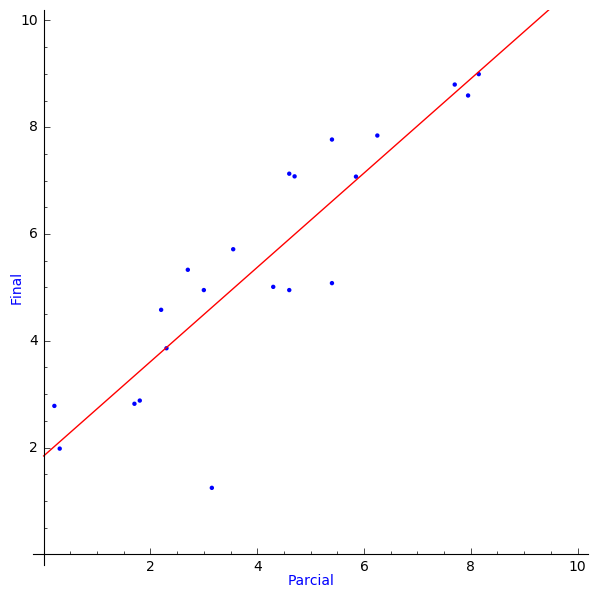
\includegraphics[width=10cm]{regre.png}}
\caption{Recta de regressió\label{fig:recta_reg}}
\end{figure}
\end{exemple}
\subsubsection{Cas general}
En el cas general, suposem que tenim un sistema d'equacions lineals:
\[
A x = b
\]
amb $A\in M_{m\times n}(\R)$ amb $m\geq n$ (més equacions que incògnites) i tal que $\Rang(A)=n$. És molt probable que aquest sistema no tingui solució, i per aquests casos ens interessa tenir la millor aproximació:
\begin{lema}
Amb les hipòtesis anteriors, el sistema
\[
A^T A x = A^T b
\]
té solució única. Aquesta solució s'anomena \emph{solució per mínim quadrats del sistema $Ax=b$}\index{mínims quadrats}.
\end{lema}
\begin{proof}
Observem que $A^TA \in M_{n\times n}(\R)$, pel que tant sols cal veure que $\Rang(A^T A)=n$ (i llavors serà un sistema compatible determinat), o el que és el mateix, que l'aplicació lineal $f_{A^TA}$ és injectiva (llavors el sistema homogeni que té per matriu associada $A^TA$ serà compatible determinat i per tant $\Rang(A^T A)=n$). Però si $\vec u \in \R^n$ compleix $A^TA\vec u=\vec 0$, tenim $A^T(A\vec u)=\vec 0$, per tant $A\vec u$ és solució del sistema homogeni que té per matriu associada $A^T$, que és de rang $n$, per tant $A\vec u=\vec 0$. Aplicant ara que $\Rang(A)=n$, tenim que $\vec u=\vec 0$ i per tant $\Rang(A^TA)=n$.
\end{proof}
\begin{lema}
Continuem amb les hipòtesis anteriors.
De tots els vectors $\vec v \in \R^n$, la solució per mínims quadrats del sistema $Ax=b$ és la que és més propera a $v$ en el sentit següent: si $x$ és la solució del sistema $A^TAx=A^Tb$ i $v\in \R^n$, llavors 
\[
||Ax - b||^2 \leq ||Av- b||^2.
\]
\end{lema}
\begin{proof}
Es dedueix del fet que la solució per mínims quadrats sigui la projecció ortogonal de $b$ a l'espai generat per les columnes d'$A$, que, com que el rang d'$A$ és $n$, queda caracteritzada per complir:
\[
A^T(Ax-b)=\vec 0 .
\]
\end{proof}
D'aquí també es dedueix que la projecció del vector $b$ a $V$, el subespai generat per les columnes d'$A$ és, en la base de $V$ formada per les columnes d'$A$ és:
\[
x=(A^TA)^{-1}A^Tb
\]
Per tant, el vector d'$\R^n$ és:
\[
Ax=A(A^TA)^{-1}A^Tb
\]
I per tant:
\begin{proposicio}
Si $V\subset \R^n$ és un subespai vectorial i $[\vec v_1, \dots , \vec v_k]$ és una base de $V$, la projecció de $\R^n$ a $V$ ve donada per la matriu:
\[
[\proj_V]=A(A^TA)^{-1}A^T
\]
on $A$ és la matriu que té per columnes els vectors $\vec v_j$.
\end{proposicio}
\begin{exemple}
Suposem que tenim un grup de 24 estudiants als que s'ha fet una avaluació parcial i un lliurament a mig semestre amb les notes següents. La tercera columna diu quina ha sigut la nota final de l'assignatura (amb més avaluacions entremig):
\[
\begin{array}{|c|c|c||c|c|c|}
\hline \text{Lliurament} & \text{Parcial} & \text{Final} & 
\text{Lliurament} & \text{Parcial} & \text{Final}\\ \hline
9.25 & 9.75 & 8.25 & 
9.5 & 5.2 & 7.27 \\
9.5 & 2.4 & 3.66 &
9 & 7.1 & 8.32 \\
8 & 1.6 & 5.65 &
8 & 4 & 7.61 \\
8 & 7.1 & 6.71 &
8.5 & 3.4 & 6.77 \\
8.5 & 5.7 & 7.77 &
8 & 6 & 7.74 \\
6 & 2.9 & 6.5 &
10 & 5.9 & 8.37 \\
9 & 9 & 8.13 &
10 & 2.6 & 8.13 \\
8 & 7.6 & 7.15 &
7.5 & 1.6 & 5.21 \\
9 & 6.2 & 6.8 &
10 & 9 & 8.52 \\
10 & 10 & 9.07 &
9 & 8 & 7.76 \\
9 & 6.5 & 7.43 &
9.75 & 10 & 8.71 \\
8.5 & 4 & 6.39 &
9.5 & 7.4 & 8.57 \\ \hline
\end{array}
\]
Volem aproximar la nota final a partir de les dues que se saben a mig semestre mitjançant una formula:
\[
\text{final} = a * \text{Lliurament} + b * \text{Parcial} + c
\]
I per tant, fem mínim quadrats per trobar $a,b$ i $c$.
En aquest cas, el sistema que té moltes més equacions que incògnites seria:
\[
\begin{pmatrix}
9.25 & 9.75 & 1 \\
9.5 & 2.4 & 1 \\
8 & 1.6 & 1 \\
\vdots & \vdots & \vdots \\
9.5 & 7.4 & 1
\end{pmatrix}
\begin{pmatrix} a \\ b \\ c \end{pmatrix}=
\begin{pmatrix} 8.25 \\ 3.66 \\ 5.65 \\ \vdots \\ 8.57 \end{pmatrix}
\]
I per tant hem de resoldre el sistema compatible determinat:
\[
\begin{pmatrix}
9.25 & 9.5 & 8 & \cdots & 9.5 \\
9.75 & 2.4 & 1.6 & \cdots & 7.4 \\
1 & 1 & 1 & \cdots & 1
\end{pmatrix}
\begin{pmatrix}
9.25 & 9.75 & 1 \\
9.5 & 2.4 & 1 \\
8 & 1.6 & 1 \\
\vdots & \vdots & \vdots \\
9.5 & 7.4 & 1
\end{pmatrix}
\begin{pmatrix} a \\ b \\ c \end{pmatrix}=
\begin{pmatrix}
9.25 & 9.5 & 8 & \cdots & 9.5 \\
9.75 & 2.4 & 1.6 & \cdots & 7.4 \\
1 & 1 & 1 & \cdots & 1
\end{pmatrix}
\begin{pmatrix} 8.25 \\ 3.66 \\ 5.65 \\ \vdots \\ 8.57 \end{pmatrix}
\]
Quedant:
\[
\left(\begin{array}{ccc}
1885.375 & 1287.5375 & 211.5 \\
1287.5375 & 1015.0425 & 142.95 \\
211.5 & 142.95 & 24
\end{array}\right)
\begin{pmatrix} a \\ b \\ c \end{pmatrix}=
\begin{pmatrix}
1568.205 \\ 1108.1755 \\ 176.49
\end{pmatrix}
\]
Que té per solució (amb 3 decimals):
\[
\begin{pmatrix} a \\ b \\ c \end{pmatrix}=
\begin{pmatrix} 0.191 \\
0.316 \\
3.790 \end{pmatrix}
\]
Per ant l'aproximació és:
\[
\text{final} = 0.191 * \text{Lliurament} + 0.316 * \text{Parcial} + 3.79\, .
\]
Per exemple, d'un alumne que tregui un $4$ al lliurament i un altre $4$ al parcial, aquest model diu que de l'assignatura acabés amb un $5.817$
\end{exemple}


\subsection{Formes bilineals i productes escalars}
% Més abstracte
\begin{definicio}
Donat un espai vectorial $E$ sobre un cos $\K$, una \emph{forma bilineal}\index{forma bilineal} és una aplicació
\[
\phi \colon E \times E \to \K
\]
tal que:
\begin{itemize}
\item $\phi(\vec u_1+\vec u_2,v)=\phi(\vec u_1,\vec v)+\phi(\vec u_2,\vec v)$ per a tots $\vec u_1$, $\vec u_2$ i $\vec v$ d'$E$,
\item $\phi(\lambda \vec u,\vec v)=\lambda \phi(\vec u,\vec v)$ per a tots $\vec u$ i $\vec v$ d'$E$ i $\lambda \in \K$,
\item $\phi(\vec u,\vec v_1,\vec v_2)=\phi(\vec u,\vec v_1)+\phi(\vec u,\vec v_2)$ per a tots $\vec u$, $\vec v_1$ i $\vec v_2$ d'$E$ i
\item $\phi(\vec u,\lambda \vec v)=\lambda \phi(\vec u,\vec v)$ per a tots $\vec u$ i $\vec v$ d'$E$ i $\lambda \in \K$.
\end{itemize}
A més diem que una aplicació bilineal $\phi$ és:
\begin{itemize}
    \item \emph{simètrica}\index{forma bilineal!simètrica} si $\phi(\vec u,\vec v)=\phi(\vec v,\vec u)$ per a tots $\vec u$ i $\vec v$ d'$E$,
    \item \emph{degenerada}\index{forma bilineal!degenerada} si existeix $\vec u\neq \vec 0$ tal que $\phi(\vec u,\vec v)=0$ per a tot $\vec v$ d'$E$, i
    \item \emph{definida positiva}\index{forma bilineal!definida positiva} si $\phi(\vec u,\vec u)>0$ per a tot $\vec u\neq \vec 0$.
\end{itemize}
\end{definicio}
\begin{definicio}\label{def:mat_apl_bil}
Si $E$ és un $\K$-espai vectorial de dimensió finita i $\calb=[\vec v_1, \dots, \vec v_n]$ és una base d'$E$, i $\phi$ és una aplicació bilineal, \emph{la matriu de l'aplicació bilineal en la base $\calb$}\index{aplicació bilineal!matriu}\index{matriu!aplicació bilineal} és:
\[
[\phi]_\calb= \begin{pmatrix}
\phi(\vec v_1,\vec v_1) & \phi(\vec v_1,\vec v_2) & \cdots & \phi(\vec v_1,\vec v_n)\\
\phi(\vec v_2,\vec v_1) & \phi(\vec v_2,\vec v_2) & \cdots & \phi(\vec v_2,\vec v_n)\\
\vdots & \vdots & \ddots & \vdots \\
\phi(\vec v_n,\vec v_1) & \phi(\vec v_n,\vec v_2) & \cdots & \phi(\vec v_n,\vec v_n)
\end{pmatrix}.
\]
\end{definicio}
\begin{lema}
Si $\phi$ és una aplicació bilineal definit sobre un $\K$-espai vectorial $E$ amb base  $\calb=[\vec v_1, \dots, \vec v_n]$ i $[\phi]_\calb$ és la matriu de $\phi$ en la base $\calb$, llavors: si $\vec u$ i $\vec w$ són vectors d'$E$ amb coordenades en la base $\calb$:
\[
[\vec u]_\calb = \begin{pmatrix}
\lambda_1 \\ \vdots \\ \lambda_n
\end{pmatrix}
\text{ i }
[\vec w]_\calb = \begin{pmatrix}
\mu_1 \\ \vdots \\ \mu_n
\end{pmatrix}.
\]
llavors:
\[
\phi(\vec u,\vec w)=\sum_{i=1}^n \sum_{j=1}^n \lambda_i\mu_j\phi(\vec v_i,\vec v_j) =[\vec u]_\calb^T \, [\phi]_\calb \, [\vec w]_\calb .
\]
\end{lema}
\begin{proof}
La primera igualtat és per bilinealitat, i és igual a l'última expressió, que està escrita en forma matricial.
\end{proof}
\begin{lema}\label{lema:canvi_base_forma_bil}
Si tenim $\calb=[\vec v_1, \dots, \vec v_n]$ i $\calc=[\vec u_1,\dots, \vec u_n]$ bases de $\K^n$, $[\Id_n]_{\calc,\calb}$ la matriu del canvi de base (la que té per columnes les coordenades dels vectors $\vec u_j$  en la base $\calb$), i $\phi$ una aplicació bilineal, hi ha la relació següent entre les matrius de l'aplicació bilineal en cada base:
\[
[\phi]_\calc=[\Id_n]_{\calc,\calb}^T \, [\phi]_\calb \, [\Id_n]_{\calc,\calb} 
\]
\end{lema}
\begin{proof}
Les matrius de $[\phi]_\calb$ i $[\phi]_\calc$ han de complir que, per a tot $\vec u$ i $\vec v$ de $\K^n$ es compleixi:
\begin{equation}\label{eq:canvi_base_apl_bil}
[\vec u]_\calc^T \, [\phi]_\calc \, [\vec v]_\calc = \phi(\vec u, \vec v)=  [\vec u]_\calb^T\, [\phi]_\calb\, [\vec v]_\calb .
\end{equation}
Però, per les propietats de la matriu $[\Id]_{\calc,\calb}$ tenim:
\[
[\vec u]_\calb=[\Id]_{\calc,\calb} [\vec u]_\calc ,
\]
i si ho substituïm a l'Equació \eqref{eq:canvi_base_apl_bil}, tenim, que per a tot $\vec u$ i $\vec v$ de $\K^n$:
\[
[\vec u]_\calc^T \, [\phi]_\calc \, [\vec v]_\calc = ([\Id]_{\calc,\calb} [\vec u]_\calc)^T \, [\phi]_\calb \, ([\Id]_{\calc,\calb} [\vec v]_\calc) = [\vec u]_\calc^T \, ([\Id]_{\calc,\calb}^T [\phi]_\calb [\Id]_{\calc,\calb}) \, [\vec v]_\calc ,
\]
pel que tenim la igualtat de matrius que volem.
\end{proof}
\begin{exemple}
Considerem la forma bilineal simètrica $\phi\colon \R^2 \times \R^2 \to \R$ donada per la matriu (en la base estàndard $\calb=[\vec e_1,\vec e_2]$)
\[
[\phi]=\begin{pmatrix} 0 & 1/2 \\ 1/2 & 0 \end{pmatrix}
\]
I volem calcular la matriu de $\phi$ en la base $\calc=[\smat{1\\1},\smat{1\\-1}]$. Llavors hem de calcular:
\[
[\Id]_{\calc,\calb}=\begin{pmatrix} 1 & 1 \\ 1 & -1 \end{pmatrix}
\]
I per tant la matriu
\[
[\phi]_\calc = \begin{pmatrix} 1 & 1 \\ 1 & -1 \end{pmatrix}^T
\begin{pmatrix} 0 & 1/2 \\ 1/2 & 0 \end{pmatrix}
\begin{pmatrix} 1 & 1 \\ 1 & -1 \end{pmatrix}=
\begin{pmatrix} 1 & 0 \\ 0 & -1 \end{pmatrix}.
\]
Per tant, les matrius $\smat{0 & 1/2 \\ 1/2 & 0}$ i $\smat{1 & 0 \\ 0 & -1}$ representen la mateixa forma bilineal en bases diferents.
\end{exemple}

Mirem ara un cas particular de forma bilineal:

\begin{definicio}
Un \emph{producte escalar}\index{producte escalar} sobre un $\R$-espai vectorial $E$ és una forma bilineal simètrica definida positiva. En general, escriurem el resultat amb un punt: $\vec u \cdot \vec v$.
\end{definicio}
Si $\calb$ és una base finita d'un espai vectorial $E$ i $\cdot$ és un producte escalar, la matriu $[\cdot]_\calb$ serà simètrica.
\begin{exemple}
Si considerem $\R^n$ i $\calb=[\vec e_1, \dots, \vec e_n]$ la base estàndard, el producte escalar definit com $\vec u \cdot \vec v=\vec u^T \vec v$ és un producte escalar amb matriu la matriu identitat $\1_n$.
\end{exemple}

\begin{exemple}
Si $E=C^\infty(\R)$ definim el producte escalar:
\[
f\cdot g = \int_{-1}^1 f(x)g(x)\mathrm{d}x .
\]
Com que a $C^\infty(\R)$ no hi ha una base finita, no té sentit parlar de la matriu del producte escalar.
\end{exemple}

\begin{exemple}\label{exemple:complexos}
Considerem els nombres complexos $\C$\index{nombres complexos}. Definits com $\R$ espai vectorial, tenen dimensió $2$ i una base és $[1,i]$, i d'aquí deduïm l'estructura de la suma. A més, però, es poden multiplicar,  i la multiplicació ve caracteritzada pel fet $i^2=-1$ i que sigui commutativa i distributiva amb la suma: o sigui,
\[
\C = \{ a + bi \mid a \in\R, b \in\R \}
\]
amb les operacions:
\[
(a+bi)+(c+di)=(a+c)+(b+d)i \text{ i } (a+bi)(c+di)=(ac-bd)+(ad+bc) i .
\]
Veiem que $\R\subset \C$, considerant el números de la forma $a+0i$.

Si $z=a+bi$, amb $a$ i $b$ reals, és un nombre complex, definim el \emph{conjugat de $z$}\index{conjugat} i escrivim $\overline z$ com:
\[
\overline z = a-bi .
\]
Veiem que:
\begin{itemize}
    \item $z \overline z=a^2+b^2\in \R$, 
    \item $z=\overline{z} \iff z\in\R$,
    \item $\overline{z_1 + z_2}=\overline{z_1}+\overline{z_2}$ i
    \item $\overline{z_1 z_2}=\overline{z_1}\, \overline{z_2}$.
\end{itemize}

Considerem ara $\C^n$ com a $\C$-espai vectorial de dimensió $n$ (suma coordenada a coordenada i multiplicació per un escalar a totes les coordenades). Definim la forma bilineal següent:
\[
\text{si }
\vec v=\begin{pmatrix}
v_1 \\ \vdots \\ v_n
\end{pmatrix}
\text{ i }
\vec w=\begin{pmatrix}
w_1 \\ \vdots \\ w_n
\end{pmatrix}
\text{ llavors }
\vec v\cdot \vec w= \sum_{i=1}^n v_i\overline{w}_i=\vec v^T \overline{\vec w} \text{ on }
\overline{\vec w}=\begin{pmatrix}
\overline w_1 \\ \vdots \\ \overline w_n
\end{pmatrix}.
\]
Que compleix, a més de les propietats de ser forma bilineal:
\begin{itemize}
    \item $\vec v\cdot \vec w$=$\overline{\vec w\cdot \vec v}$ per a tot $\vec v,\vec w\in \C^n$ (diem que és hermítica\index{forma!hermítica}) i
    \item $\vec v\cdot \vec v=||\vec v||^2\in \R$ per a tot $\vec v\in\C^n$.
\end{itemize}
\end{exemple}

\subsection{Tota matriu simètrica sobre \texorpdfstring{$\mathbb{R}$}{R} diagonalitza}
El resultat que volem demostrar a aquest apartat és:
\begin{teorema}[Teorema espectral]
Una matriu $A\in M_n(\R)$ diagonalitza en una base ortonormal si, i només si, $A$ és simètrica.
\end{teorema}
Per demostrar el teorema espectral necessitem utilitzar el \emph{Teorema fonamental de l'àlgebra}, que no demostrem aquí perquè la seva demostració surt dels objectius del curs:
\begin{teorema}[Teorema fonamental de l'àlgebra]
Si $p(x)\in\C[x]$ ($p(x)$ és un polinomi amb coeficients a $\C$) de grau $\geq 1$, existeix $z\in C$ tal que $p(z)=0$.
\end{teorema}
\begin{proof}[Demostració del teorema espectral]
Una implicació és directa: si $A$ diagonalitza en una base ortonormal vol dir que podem escriure:
\[
A=Q D Q^T
\]
amb $D$ una matriu diagonal i $Q$ una matriu ortogonal ($Q^{-1}=Q^T$). Per tant:
\[
A^T=(QDQ^T)^T=(Q^T)^T D^T Q^T=Q D^T Q^T=A
\]
i $A$ és simètrica.

Per demostrar l'altra implicació, ho farem per inducció sobre $n$:
\begin{itemize}
    \item Per a $n=1$, tota matriu és simètrica i diagonal.
    \item Suposem cert per a $n-1$, i volem demostrar-ho per $n$: considerem $A\in M_n(\R)$ i $p_A(x)$ el polinomi característic. Pensem $p_A(x)\in\C[x]$ i, pel teorema fonamental de l'àlgebra, existeix $\lambda \in \C$ tal que $p_A(\lambda)=0$. També tindrem un vector propi $\vec v\in \C^n$ tal que $A \vec v=\lambda \vec v$.
    
    Considerem ara la forma bilineal hermítica definida a l'Exemple \ref{exemple:complexos}:
    \[
    A\vec v \cdot \vec v = \lambda \vec v \cdot \vec v= \lambda ||\vec v||^2 \text{ amb $0\neq ||v||^2\in R$}.
    \]
    Però també:
    \[
    A\vec v \cdot\vec  v = (A \vec v)^T \overline{\vec v} = \vec v^T A^T \overline{\vec v} = \vec v^T \overline{(\overline{A^T} \vec v)} = \vec v^T A \overline{\vec v} = \vec v^T (\overline{\lambda \vec v})=\overline{\lambda} ||\vec v||^2 , 
    \]
    on hem utilitzat que $A=A^T$ ($A$ és simètrica) i $\overline A=A$ ($A$ té coeficients reals).
    
    Per tant, tenim que $\lambda=\overline{\lambda}$ i obtenim $\lambda \in \R$.
    
    Com que $p_A(\lambda)=0$, tenim que existeix un vector propi real $\vec v\neq \vec 0$ tal que $A\vec v=\lambda \vec v$. Podem considerar que $||\vec v||=1$ (si cal, substituïm $\vec v$ per $\frac{1}{||\vec v||}\vec v$).
    
    Ampliem $\vec v$ amb $\vec v_2$, \dots, $\vec v_n$ de tal manera que $[\vec v,\vec v_2, \dots ,\vec v_n]$ sigui una base ortonormal (primer ampliem fins a base, i després apliquem Gram-Schmidt). Si considerem $Q$ la matriu que té per columnes els vectors $\vec v$, $\vec v_2$, \ldots , $\vec v_n$, tenim:
    \[
    QAQ^T=\begin{pmatrix} \lambda & b_{12} & \cdots & b_{1n} \\
    0 & b_{22} & \cdots & b_{2n} \\
    \vdots & \vdots & \ddots & \vdots \\
    0 & b_{n2} & \cdots  & b_{nn}
    \end{pmatrix}
    \]
    on hem utilitzat que $Q^{-1}=Q^T$. Però com que $A=A^T$, tenim $(QAQ^T)^T=QAQ^T$, i per tant $b_{12}=b_{13}=\cdots=b_{1n}=0$.
    
    Ara restringim l'aplicació $f_A$ a l'espai $\langle v_2, \dots , v_n\rangle$, que en la base $[v_2, \dots , v_n]$ té per matriu
    \[
    B=\begin{pmatrix} b_{22} & \cdots & b_{2n} \\
    \vdots & \ddots & \vdots \\
    b_{n2} & \cdots  & b_{nn}
    \end{pmatrix}
    \]
    que és simètrica i $B\in M_{n-1}(\R)$. Per hipòtesis d'inducció, $B$ diagonaliza en una base ortonormal, pel que existeix $P\in M_{n-1}(\R)$ matriu ortogonal i $D$ matriu diagonal tals que $B=P^TDP$. Amb això tenim:
    \[
    QAQ^T=\left(\begin{array}{c|c}
        \lambda & 0 \\ \hline
        0 & P^T D P
    \end{array}\right)=
    \left(\begin{array}{c|c}
        1 & 0 \\ \hline
        0 & P^T
    \end{array}\right)
    \left(\begin{array}{c|c}
        \lambda & 0 \\ \hline
        0 & D 
    \end{array}\right)
    \left(\begin{array}{c|c}
        1 & 0 \\ \hline
        0 &  P
    \end{array}\right)
    \]
    Per tant, considerem
    \[
    Q'=\left(\begin{array}{c|c}
        1 & 0 \\ \hline
        0 &  P
    \end{array}\right) Q \text{ i }
    D'=\left(\begin{array}{c|c}
        \lambda & 0 \\ \hline
        0 & D 
    \end{array}\right)
    \]
    i tenim que $Q'$ és una matriu ortogonal i $A=Q'^{-1} D' Q'$, amb $D'$ una matriu diagonal, pel que $A$ diagonalitza a una base ortonormal.
    \end{itemize}
\end{proof}

\subsection{Descomposició en valors singulars}
A aquest apartat resoldrem la pregunta següent amb les eines que hem vist: si $f=f_A\colon \R^n \to \R^m$ és una aplicació lineal, existeix una base ortonormal $\calb=[\vec v_1, \dots, \vec v_n]$ d'$\R^n$ tal que $f(\vec v_1), \dots, f(\vec v_n)$ siguin ortogonals?

Veurem que sí:
\begin{teorema}\label{teo:val_sing}
$f=f_A\colon \R^n \to \R^m$ és una aplicació lineal, llavors existeix una base ortonormal $\calb=[\vec v_1, \dots, \vec v_n]$ d'$\R^n$ tal que $f(\vec v_1), \dots, f(\vec v_n)$ tal que són ortogonals.
\end{teorema}
\begin{proof}
Considerem $f=f_A$, i per tant $A\in M_{m\times n}(\R)$ la matriu tal que $f(\vec v)=A\vec v$. Llavors, la matriu $A^TA\in M_n(\R)$ és simètrica, i per tant diagonalitza en una base ortonormal, per tant, existeix una base ortonormal $\calb[\vec v_1, \dots, \vec v_n]$ de $\R^n$ i escalars $\lambda_1, \dots, \lambda_n\in \R$ tals que
\[
A^T A \vec v_i=\lambda_i \vec v_i \text{ per a tot $i=1, \dots, n$.}
\]
Volem veure que $f(\vec v_1), \dots, f(\vec v_n)$ són ortogonals, o sigui, $f(\vec v_i)\cdot f(\vec v_j)=0$ si $i\neq j$:
\begin{align*}
f(\vec v_i)\cdot f(\vec v_j) & =(A\vec v_i)\cdot(A\vec v_j)=(A\vec v_i)^T(A\vec v_j)=(\vec v_i^T A^T)(A \vec v_j)= \\
 &  = \vec v_i^T (A^T A \vec v_j)=\vec v_i^T (\lambda_j \vec v_j)=\lambda_j (\vec v_i \cdot \vec v_j)=0 .
\end{align*}
\end{proof}
\begin{observacio}
El Teorema~\ref{teo:val_sing} no diu que $\calb$ sigui única, i de fet, en general, no ho és: considereu l'aplicació identitat de $\R^n \to \R^n$, que envia qualsevol base ortonormal a vectors ortogonals.
\end{observacio}

 La interpretació geomètrica a $\R^2$ és la següent: la imatge d'una circumferència de radi $1$ centrada a l'origen és una el·lipsi, els vectors propis d'$A^TA$ corresponen a les direccions principals de l'el·lipsi, i les longituds dels semieixos principals són les arrels quadrades dels valors propis d'$A^TA$. Posem nom a aquests valors:
 \begin{definicio}
 Donada una matriu $A\in M_{m\times n}(\R)$, definim els \emph{valors singulars d'$A$}\index{valors singulars} com les arrels quadrades dels valors propis de la matriu $A^TA$: $\sigma_1, \dots, \sigma_m$ positius tals que $\sigma_i^2$ és valor propi d'$A^TA$.
 \end{definicio}
 \begin{observacio}
 $\sigma_i$ és el mòdul $||f(\vec v_i)||$ a l'enunciat del Teorema \ref{teo:val_sing}.
 \end{observacio}
 \begin{proposicio}
 Si $f=f_A\colon \R^n \to \R^m$ és una aplicació lineal i $\Rang(A)=r$, llavors hi ha $r$ valors singulars diferent de zero i els $n-r$ restants valen zero.
 \end{proposicio}
\begin{proof}
Tenim que en la base $\calb$ del Teorema \ref{teo:val_sing}, $f_A$ té per matriu $[f_A]\calb$, una matriu amb $\sigma_i$ a la diagonal i zeros a la resta. Llavors, com que el rang és la dimensió de la imatge, el rang de $f_A$  és igual al de $[f_A]_\calb$, que és el nombre de $\sigma_i$ no nuls, i la resta han de ser zero.
\end{proof}

Podem aprofitar aquests raonaments per demostrar:
\begin{teorema}\label{teo:SVD}
Si $A\in M_{m\times n}(\R)$, llavors existeixen $P \in M_{m}(\R)$ ortogonal, $D\in M_{m\times n}(\R)$ amb els únics elements no nuls a la diagonal i positius, i $Q\in M_n(\R)$ ortogonal tals que:
\[
A=PDQ.
\]
A més, podem ordenar les entrades diagonals de $D$ de més gran a més petita. Anomenem a aquesta descomposició com una \emph{descomposició en valors singulars d'$A$}\index{descomposició en valors singulars}.
\end{teorema}
\begin{proof}
Considerem l'aplicació lineal $f_A$ i veiem que necessitem bases ortonormals $\calb$ d'$\R^n$ i $\calc$ d'$\R^m$ tals que $D=[f_A]_{\calb,\calc}$ sigui diagonal.

El Teorema \ref{teo:val_sing} ens dóna una base $\calb$ d'$\R^n$ que és ortonormal. Ordenem aquesta base de tal manera que $||f(\vec v_i)||\geq ||f(\vec v_{i+1})||$. Sigui $Q^T=Q^{-1}$ la matriu que té per columnes aquesta base.

Els vectors $f(\vec v_1), \dots, f(\vec v_n)$ són ortogonals. Suposem que els $k$ primers són no nuls, llavors, considerant:
$\vec w_i=\frac{1}{||f(\vec v_i)||}$ per a $1\leq i \leq k$, tindrem vectors ortonormals d'$\R^m$, per tant linealment independents, i que podem ampliar amb $\vec w_{k+1}, \dots, \vec w_m$ fins a tenir una base ortonormal $\calc$ d'$\R^m$. Sigui $P$ la matriu que té per columnes aquests vectors.

Com que $f(\vec v_i)=||f(\vec v_i)|| \vec w_i$ si $i\leq k$ i $f(\vec v_i)=\vec 0$ si $i>k$, tenim que $[f]_{\calb,\calc}$ és diagonal amb els valors singulars d'$A$ a la diagonal ordenats de més gran a més petit.
\end{proof}

\begin{exemple}
Considerem l'aplicació lineal $f_A\colon \R^2 \to \R^2$ amb:
\[
A=\begin{pmatrix}
3 & -9/5 \\ -1 & 13/5
\end{pmatrix}
\]
i volem fer-ne una descomposició en valors singulars.

Calculem primer $A^TA$:
\[
A^T A = \begin{pmatrix}
10 & -8 \\ -8 & 10
\end{pmatrix}
\]
I la diagonalitzem. El polinomi característic és:
\[
p_{A^TA}(x)=x^2 - 20 x + 36 = (x-18)(x-2)
\]
Per tant, els valors propis d'$A^TA$ són $\lambda_1=18$ i $\lambda_2=2$ i els corresponents vectors propis:
\[
\Ker(A^TA-18\1_2)=\langle \begin{pmatrix} 1 \\ -1 \end{pmatrix} \rangle \text{ i }
\Ker(A^TA-2\1_2)=\langle \begin{pmatrix} 1 \\ 1 \end{pmatrix} \rangle
\]
I com que els hem de considerar unitaris, obtenim:
\[
Q^T=\begin{pmatrix}
1/\sqrt{2} & 1/\sqrt{2} \\ -1/\sqrt{2} & 1/\sqrt{2}
\end{pmatrix}
\text{ i per tant }
Q=\begin{pmatrix}
1/\sqrt{2} & -1/\sqrt{2} \\ 1/\sqrt{2} & 1/\sqrt{2}
\end{pmatrix}.
\]

La matriu diagonal són els valors singulars, que són les arrels quadrades dels valors propis d'$A^TA$, per tant són $\sigma_1=\sqrt{18}=3\sqrt{2}$ i $\sigma_2=\sqrt{2}$ i tenim:
\[
D=\begin{pmatrix}
3\sqrt{2} & 0 \\ 0 & \sqrt{2}
\end{pmatrix}.
\]

I la matriu $P$ té per columnes les imatges de $\smat{1\\-1}$ i $\smat{1\\1}$ per $f_A$ dividides per les seves normes, per tant:
\[
\begin{pmatrix}
3 & -9/5 \\ -1 & 13/5
\end{pmatrix} 
\begin{pmatrix}
1 \\ -1 
\end{pmatrix}=
\begin{pmatrix}
24/5 \\ -18/5
\end{pmatrix}=
6 \begin{pmatrix}
4/5 \\ -3/5
\end{pmatrix}
\]
i
\[
\begin{pmatrix}
3 & -9/5 \\ -1 & 13/5
\end{pmatrix} 
\begin{pmatrix}
1 \\ 1 
\end{pmatrix}=
\begin{pmatrix}
6/5 \\ 8/5
\end{pmatrix}=
2 \begin{pmatrix}
3/5 \\ 4/5
\end{pmatrix}
\]
Per tant:
\[
P=\begin{pmatrix}
4/5 & 3/5 \\ -3/5 & 4/5
\end{pmatrix}
\]
I una descomposició d'$A$ en valors singulars és:
\[
\begin{pmatrix}
3 & -9/5 \\ -1 & 13/5
\end{pmatrix} 
=\begin{pmatrix}
4/5 & 3/5 \\ -3/5 & 4/5
\end{pmatrix} 
\begin{pmatrix}
3\sqrt{2} & 0 \\ 0 & \sqrt{2}
\end{pmatrix}
\begin{pmatrix}
1/\sqrt{2} & -1/\sqrt{2} \\ 1/\sqrt{2} & 1/\sqrt{2}
\end{pmatrix}.
\]
A la Figura \ref{fig:circ_ellipse} podem veure com es modifica la circumferència unitat quan apliquem la matriu $A$. Veiem que a la direcció $\smat{4\\-3}$ hi ha el primer eix principal amb semilongitud $3\sqrt{2}$ i a la direcció $\smat{3\\4}$ l'altre eix, amb semilongitud $\sqrt{2}$.
\begin{figure}[ht]
\center{
\begin{tabular}{ccc}
\begin{minipage}{5cm}{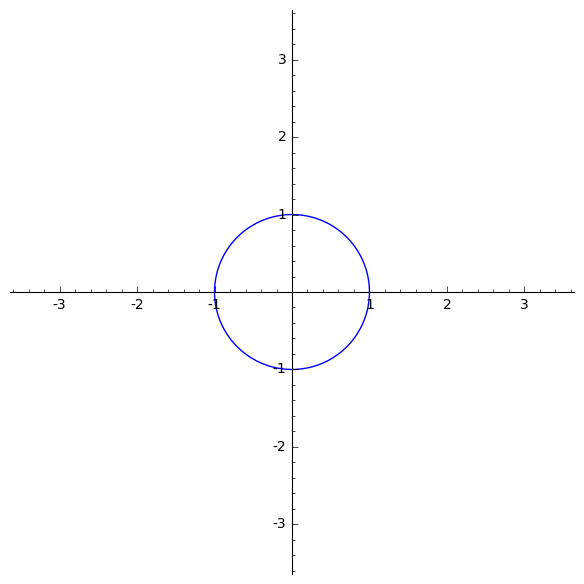
\includegraphics[width=\textwidth]{cercle.png}}\end{minipage}  & $\Rightarrow$ & \begin{minipage}{5cm}{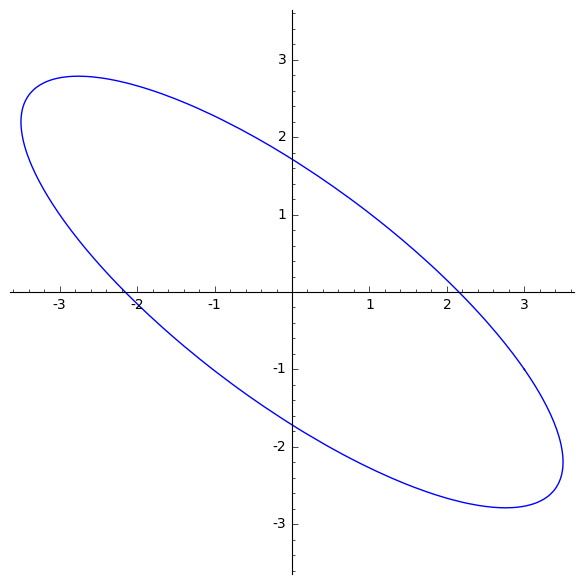
\includegraphics[width=\textwidth]{ellipse.png}}\end{minipage}
\end{tabular}}
\caption{Deformació de la circumferència unitat per l'aplicació lineal $f_A$.\label{fig:circ_ellipse}}
\end{figure}
\end{exemple}

\subsection{Classificació de formes bilineals simètriques sobre \texorpdfstring{$\mathbb{R}^n$}{Rn}}
A aquesta secció l'objectiu és classificar les formes bilineals. Definim abans què vol dir que siguin equivalents:
\begin{definicio}
Diem que dues formes bilineals $\phi_1,\phi_2\colon \K^n\times\K^n\to \K$ amb matrius corresponents $[\phi_1]$ i $\phi_2]$ \emph{són equivalents} si existeix una base $\calc$ de $\K^n$ tal que
\[
[\phi_1]=[\phi_2]_\calc .
\]
Dit d'una altra manera, si existeix una matriu invertible $\cals\in M_n(\K)$ (la matriu del canvi de base, que té per columnes els vectors de $\calc$) tal que
\[
[\phi_1]=\cals^T [\phi_2] \cals.
\]
Escriurem $q_1\sim q_2$.
\end{definicio}
\begin{lema}
Ser equivalents com a formes bilineals de $\K^n\times \K^n$ a $\K$ és una relació d'equivalència. O sigui:
\begin{itemize}
    \item $\phi \sim \phi$ per a tot $\phi$ forma bilineal (reflexiva),
    \item $\phi_1\sim \phi_2 \Leftrightarrow \phi_2 \sim \phi_1$ per a totes $\phi_1, \phi_2$ formes bilineals (simètrica) i
    \item $\phi_1\sim \phi_2$ i $\phi_2\sim \phi_3$ implica $\phi_1\sim \phi_3$ per a totes $\phi_1,\phi_2,\phi_3$ formes quadràtiques (transitiva).
\end{itemize}
\end{lema}
\begin{proof}
Cal veure en cada cas quina és la matriu $\cals$ del canvi de base:
\begin{itemize}
    \item Per veure que $\phi\sim \phi$, considerem $\cals=\1_n$,
    \item Si $\phi_1\sim \phi_2$ tenim que existeix $\cals$ una matriu de canvi de base (i per tant invertible) tal que:
    \[
    [\phi_1]=\cals^T [\phi_2] \cals.
    \]
    Però aquesta igualtat també es pot escriure com:
    \[
    [\phi_2]=(\cals^{-1})^T [\phi_1] \cals^{-1}
    \]
    i per tant $\phi_2\sim \phi_1$.
    \item Per hipòtesis tenim que existeixen $\cals_1$ i $\cals_2$ tals que:
    \[
    [\phi_1]=\cals_1^T [\phi_2] \cals_1
    \text{ i }
    [\phi_2]=\cals_2^T [\phi_3] \cals_2.
    \]
    Llavors:
    \[
    [\phi_1]=\cals_1^T \cals_2^T [\phi_3] \cals_2 \cals_1=
    (\cals_2 \cals_1)^T [\phi_3] (\cals_2 \cals_1)
    \]
    i tenim $\phi_1\sim \phi_3$.
\end{itemize}
\end{proof}

A partir d'ara considerem que $\K=\R$ i l'objectiu és classificar les formes bilineals $\phi\colon \R^n\times \R^n \to \R$:
\begin{teorema}\label{teo:class_form:bilR}
Tota forma bilineal simètrica $\phi\colon \R^n\times \R^n\to \R$ és equivalent a una forma bilineal que té per matriu una matriu diagonal amb coeficients (a la diagonal): $1$ a les $r$ primeres files, $-1$ a les $s$ següents i $0$ a les $t$ últimes ($n=r+s+t$). O sigui una matriu de la forma:
\[
\begin{pmatrix}
1      & \cdots & 0 & 0 & \cdots & 0 & 0 & \cdots & 0 \\
       & \ddots &   &   & \cdots &   &   & \cdots &  \\
0      & \cdots & 1 & 0 & \cdots & 0 & 0 & \cdots & 0 \\
0      & \cdots & 0 & -1 & \cdots & 0 & 0 & \cdots & 0 \\
       &        &   &    & \ddots &   &   & \cdots &   \\
0      & \cdots & 0 &  0 & \cdots & -1 & 0 & \cdots & 0 \\
0      & \cdots & 0 &  0 & \cdots & 0 & 0 & \cdots & 0 \\
       &        &   &    & \cdots &   &   & \ddots &   \\
0      & \cdots & 0 &  0 & \cdots & 0 & 0 & \cdots & 0 
\end{pmatrix}
\]
A més, si definim la parella $(r,s)$ com la \emph{signatura de $\phi$} ($\sign(\phi)$)\index{forma bilineal! signatura}, dues formes bilineals bilineals $\phi_1,\phi_2\colon \R^n\times \R^n\to \R$ són equivalents si i només si $\sign(\phi_1)=\sign(\phi_2)$.
\end{teorema}
\begin{proof}
Considerem $[\phi]$ la matriu simètrica $n\times n$ sobre $\R$ de la forma bilineal $\phi$. Pel Teorema espectral, existeix una matriu ortogonal $Q$  i una matriu diagonal $D$ amb valors $\lambda_1, \dots, \lambda_n$ tal que:
\[
D=Q^T [\phi] Q \,.
\]
Ara fem els canvis següents:
\begin{itemize}
    \item Podem reordenar els elements de la diagonal de $D$ reordenant les columnes de $Q$: si $Q'$ és la matriu que resulta d'intercanviar les columnes $j$ i $k$ de $Q$, llavors, $Q'$ continua sent ortogonal i el producte:
    \[
    (Q')^T[\phi]Q'
    \]
    també és diagonal, però intercanviant les posicions $i$ i $j$, o sigui, els valors $\lambda_i$ i $\lambda_j$.\\
    Aprofitem aquesta propietat per reordenar la diagonal de $D$ i posar primer els $\lambda_i>o$, llavors els $\lambda_i<0$ i finalment els $\lambda_i=0$. Per tant, podem suposar que tenim $Q$ una matriu ortogonal tal que
    \[
    D=Q^T [\phi] Q \,.
    \]
    amb $D$ una matriu diagonal tal que a la diagonal té els $r$ primers coeficients positius, els $s$ següents negatius i els $t$ últims zero.
    \item Considerem $A$ la matriu diagonal següent, definida a partir dels coeficients de $D$: el coeficient $a_{ii}$ es defineix com:
    \[
    a_{ii}=\begin{cases}
    1/\sqrt{\lambda_i} & \text{si $1\leq i \leq r$,} \\
    1/\sqrt{-\lambda_i} & \text{si $r < i \leq r+s$,} \\
    1 & \text{si $r+s < i \leq n$.}
    \end{cases}
    \]
    Tenim que $A^TDA$ és una matriu diagonal amb $r$ uns a les primeres files, $s$ menys uns a les següents i zero a les últimes.\\
    Per tant:
    \[
    [\phi] \sim A^TQ^T [\phi] QA = (QA)^T [\phi] QA
    \]
    i $(QA)^T [\phi] QA$ és diagonal i com diu l'enunciat del teorema.
\end{itemize}
De moment hem vist que, com que ser equivalent a té la propietat transitiva, si $\phi_1$ i $\phi_2$ tenen la mateixa signatura, les dues són equivalents a una mateixa forma bilineal i per tant $\phi_1\sim \phi_2$.\\
Cal veure el recíproc, o el que és equivalent, que dues matrius diagonals equivalents $D$ i $D'$ amb $(r,s,t)$ i $(r',s',t')$ coeficients $1$, $-1$ i $0$ respectivament, llavors $(r,s,t)=(r',s',t')$. \\
Com que $D$ i $D'$ són equivalents, existeix $A$ una matriu invertible que té per columnes $v_i$ tal que:
\[
D'=A^T D A.
\]
Si fem el producte de la dreta, les $r$ primeres files són $||v_1||^2$ ($D$ coincideix amb la identitat a les $r$ primeres files i columnes), \ldots, $||v_r||^2$, per tant són números positius, per tant $r'\geq r$ i argumentant canviant els papers de $D$ i $D'$ (i $A$ per $A^{-1}$), tenim $r\geq r'$, pel que $r=r'$.\\
$r+s$ és el rang de $D$. Com que $D'$ és el producte de $D$ per matrius invertibles, $r+s$ també és el rand de $D'$, que és $r'+s'$, per tant, $s=s'$.\\
Finalment, $t=n-(r+s)=n-(r'+s')=t'$.
\end{proof}
\begin{exemple}\label{exemple:class_form_bil}
Considerem la forma bilineal $\phi\colon \R^4\times\R^4\to\R$ donada per la matriu:
\[
[\phi]=\left(\begin{array}{rrrr}
1 & 5 & -1 & 3 \\
5 & 1 & 3 & -1 \\
-1 & 3 & 1 & 5 \\
3 & -1 & 5 & 1
\end{array}\right).
\]
Una manera de classificar-la és de calcular el polinomi característic i estudiar el signe dels valors on s'anul·la:
\[
p_{[\phi]}(x)=\det(A-x\1_4)=x^{4} - 4 x^{3} - 64 x^{2} + 256 x .
\]
I $p_{[\phi]}(x)$ s'anul·la als valors $\{-8,0,4,8\}$, per tant té signatura $(2,1)$ i és equivalent a la forma bilineal que té per matriu:
\[
\begin{pmatrix} 1 & 0 & 0 & 0 \\ 0 & 1 & 0 & 0 \\ 0 & 0 & -1 & 0 \\ 0 & 0 & 0 & 0 \end{pmatrix} .
\]
\end{exemple}

Acabem aquesta secció aprofitant aquesta classificació per fer la corresponent de les formes quadràtiques.

\begin{definicio}
Una \emph{forma quadràtica}\index{forma quadràtica} sobre un cos $\K$ és una aplicació $q\colon \K^n\to \K$ que es pot expressar com:
\[
q(x_1, \dots , x_n)=\sum_{1\leq i , j \leq n} \lambda_{ij}x_i x_j
\]
amb $\lambda_{ij}\in \K$.

També es pot escriure com:
\[
q(x_1, \dots , x_n)= \vec x^T A \vec x ,
\]
on $\vec x=\smat{x_1 \\ \vdots \\ x_n}$ i $A$ és la matriu (simètrica) que té per coeficients
\[
a_{ij}=\begin{cases} \lambda_{ii} & \text{si $i=j$,} \\ \frac{\lambda_{ij}+\lambda_{ji}}{2} & \text{si $i\neq j$.}\end{cases}
\]
\end{definicio}

\begin{observacio}
Amb el que hem vist, tenim una bijecció entre les matrius simètriques (que es poden pensar com formes bilineals en una base donada) i les formes quadràtiques. Escriurem $[q]$ per denotar la matriu simètrica corresponent a la forma quadràtica $q$.
\end{observacio}
\begin{exemple}
La forma quadràtica $q\colon \R^2 \to \R$ definida per $q(x_1,x_2)=ax_1^2+bx_1x_2+cx_2^2$ correspon a la matriu simètrica
\[
\begin{pmatrix}
a & b/2 \\ b/2 & c
\end{pmatrix} .
\]
Podem recuperar la forma quadràtica fent:
\[
q(x_1,x_2)=\begin{pmatrix} x_1 & x_2 \end{pmatrix}\begin{pmatrix}
a & b/2 \\ b/2 & c
\end{pmatrix} \begin{pmatrix} x_1 \\ x_2 \end{pmatrix}=ax_1^2 + bx_1x_2+cx_2^2 .
\]
\end{exemple}
\begin{exemple}
Considerem les formes quadràtiques $q_1$ i $q_2$ de $\R^2$ a $\R$ definides com $q_1(x_1,x_2)=x_1x_2$ i $q_2(y_1,y_2)=y_1^2-y_2^2$. Observem que si fem el canvi de base:
\[
\begin{pmatrix} y_1 \\ y_2  \end{pmatrix} =
\begin{pmatrix} 1/2 & 1/2 \\ 1/2 & -1/2 \end{pmatrix}
\begin{pmatrix} x_1 \\ x_2  \end{pmatrix}
\]
es poden escriure:
\[
y_1=\frac12x_1+\frac12x_2 \text{ i } y_2=\frac12x_1-\frac12x_2 
\]
i tenim
\[
q_2(y_1,y_2)=(\frac12x_1+\frac12x_2)^2 - (\frac12x_1-\frac12x_2)^2=x_1x_2 .
\]
Per tant, tenen la mateixa forma. Aquesta igualtat també es pot veure en forma matricial observant que si $\cals$ és la matriu del canvi de base, tenim $[q_1]=\cals^T [q_2] \cals$, on $[q_1]$ i $[q_2]$ són les matrius simètriques corresponents a les formes bilineals $q_1$ i $q_2$ respectivament:
\[
\begin{pmatrix} 0 & 1/2 \\ 1/2 & 0 \end{pmatrix}=
\begin{pmatrix} 1/2 & 1/2 \\ 1/2 & -1/2 \end{pmatrix}^T
\begin{pmatrix} 1 & 0 \\ 0 & -1 \end{pmatrix}
\begin{pmatrix} 1/2 & 1/2 \\ 1/2 & -1/2 \end{pmatrix}
\]
\end{exemple}
\begin{definicio}
Diem que dues formes quadràtiques $q_1,q_2\colon \K^n\to \K$ \emph{són equivalents}, amb matrius  si existeix un canvi de base $\cals$ a $\K^n$ tal que 
\[
[q_1]=\cals^T [q_2] \cals.
\]
Escriurem $q_1\sim q_2$.
\end{definicio}

Com que els canvis de base afecten de la mateixa manera que afectaven a les formes bilineals (veure Lema \ref{lema:canvi_base_forma_bil}), obtenim que ``\emph{ser equivalent a}'' també es una relació d'equivalència a les formes quadràtiques i l'anàleg al Teorema \ref{teo:class_form:bilR}:
\begin{teorema}\label{teo:class_formQuadR}
Tota forma quadràtica $q\colon \R^n\to \R$ és equivalent a una forma bilineal del tipus:
\[
q_1(x_1,\dots, x_n)=x_1^2+ \cdots + x_r^2 - x_{r+1}^2-\cdots -x_{r+s}^2 .
\]
A més, si definim la parella $(r,s)$ com la \emph{signatura de $q$} ($\sign(q)$)\index{forma quadràtica! signatura}, dues formes quadràtiques $q_1,q_2\colon \R^n\to \R$ són equivalents si i només si $\sign(q_1)=\sign(q_2)$.
\end{teorema}
\begin{exemple}
Classifiquem la forma quadràtica $q\colon \R^4 \to \R$:
\[
q(x_1,x_2,x_3,x_4)=x_1^2+10 x_1x_2 -2 x_1x_3+6x_1x_4 + x_2^2 -6x_2x_3-2x_2x_4+x_3^3+10x_3x_4-x_4^2.
\]
Que té per matriu:
\[
\left(\begin{array}{rrrr}
1 & 5 & -1 & 3 \\
5 & 1 & 3 & -1 \\
-1 & 3 & 1 & 5 \\
3 & -1 & 5 & 1
\end{array}\right)
\]
Per tant, podem aprofitar els càlculs de l'Exemple \ref{exemple:class_form_bil}, i tenim que és equivalent a:
\[
q(y_1,y_2,y_3,y_4)=y_1^2+y_2^2-y_3^2.
\]
\end{exemple}

\begin{llista-exercicis}
\item[Secció 5.1:] 12, 16, 18.
\item[Secció 5.2:] 14, 34, 38.
\item[Secció 5.3:] 5-11, 13-20, 32.
\item[Secció 5.4:] 2, 8, 10.
\item[Secció 5.5:] 4, 10, 16, 22.
\item[Secció 8.1:] 6, 12, 16, 22.
\item[Secció 8.2:] 4, 10, 18, 22.
\item[Secció 8.3:] 6, 16, 18, 20.
\end{llista-exercicis}
}
%\appendix
%\section{Nombres complexos}
%{
%% !TeX encoding = UTF-8
% !TeX spellcheck = ca_ES-valencia
% !TeX root = MatCADAlgLin.tex

\appendix
\section{Nombres complexos}
Podem definir els nombres complexos com
\[
\C =\{a+bi ~|~ a,b\in\R\}.
\]
Com a espai vectorial sobre $\R$, podem identificar $\C$ amb $\R^2$, i per tant tenim definida una suma i una producte per reals:
\[
(a+bi) + (c+di) = (a+c) + (b+d)i, \quad \lambda(a+bi)=\lambda a + \lambda b i.
\]
Tenim però una operació addicional, el producte de nombres complexos:
\[
(a+bi)(c+di) = (ac-bd) + (ad+bc)i,
\]
on la fórmula es recorda fàcilment si tenim en compte que $i^2=-1$, i fent servir la propietat distributiva.

Definim la \emph{part real} i la \emph{part imaginària} \index{part real}\index{part imaginària} d'un nombre complex com:
\[
\Re(a+bi) = a,\quad \Im(a+bi) = b.
\]
També el \emph{conjugat}\index{conjugat} d'un nombre complex es defineix com:
\[
\overline{(a+bi)} = a-bi,
\]
i per tant tenim les fórmules
\[
\Re(z) = \frac{z+\bar z}{2},\quad \Im(z)=\frac{z-\bar z}{2i},\quad \forall z\in\C.
\]
La \emph{norma}\index{norma} d'un element $z=a+bi$ és
\[
N(z) = z\bar z = (a+bi)(a-bi) = a^2+b^2\geq 0.
\]
Observem que $z\bar z \geq 0$, i que $z\bar z = 0$ si i només si $z=0$. Això ens permet calcular fàcilment una fórmula per l'invers d'$a+bi$:
\[
(a+bi)^{-1} = \frac{1}{a+bi} = \frac{a-bi}{(a+bi)(a-bi)} = \frac{a}{a^2+b^2}+\frac{-b}{a^2+b^2}i.
\]
Pensat com un element de $\R^2$, $N(z)=|z|^2$, on $|z|=\sqrt{a^2+b^2}$ és el mòdul de $z$ pensat com un element de $\R^2$. Les coordenades polars del punt $(a,b)\in\R^2$ es calculen fent servir que:
\[
a = r\cos(\theta),\quad b = r\sin(\theta),
\]
i per tant:
\[
r = \sqrt{z\bar z}=\sqrt{a^2+b^2},\quad \theta = \arg(z) = \arctan(b/a) (+\pi),
\]
on haurem de sumar $\pi$ a $\arctan(b/a)\in[-\pi/2,\pi/2]$ si el punt $(a,b)$ pertany al II o III quadrant.

Podem escriure (aquí ho podem pensar com una notació, encara que té una justificació algebraica) que
\[
a+bi = re^{i\theta},
\]
i així podem recordar les fórmules
\[
|zw|=|z||w|,\quad \arg(zw)=\arg(z)+\arg(w)\pmod{2\pi}.
\]
El següent resultat és el motiu pel què ens interessa treballar a $\C$:

\begin{teorema}[Teorema fonamental de l'àlgebra]
Tot polinomi $f(x)\in \C[x]$ de grau $n\geq 0$ es pot escriure com
\[
f(x) = c (x-\lambda_1)\cdots (x-\lambda_n),
\]
on $c$ i $\lambda_1,\ldots,\lambda_n$ són nombres complexos (possiblement repetits).
\end{teorema}

%}

\printindex
\begin{thebibliography}{20}
\bibitem{Bret}
	Otto Bretscher,
	\textit{Linear Algebra with Applications},
	1997, Prentice-Hall International Inc.
\bibitem{NaXa}
	Enric Nart, Xavier Xarles,
	\textit{Apunts d'àlgebra lineal}, 2016, Col.lecci\'o Materials, 237, UAB.
\end{thebibliography}
\end{document}